\documentclass[twoside]{book}

% Packages required by doxygen
\usepackage{fixltx2e}
\usepackage{calc}
\usepackage{doxygen}
\usepackage[export]{adjustbox} % also loads graphicx
\usepackage{graphicx}
\usepackage[utf8]{inputenc}
\usepackage{makeidx}
\usepackage{multicol}
\usepackage{multirow}
\PassOptionsToPackage{warn}{textcomp}
\usepackage{textcomp}
\usepackage[nointegrals]{wasysym}
\usepackage[table]{xcolor}

% Font selection
\usepackage[T1]{fontenc}
\usepackage[scaled=.90]{helvet}
\usepackage{courier}
\usepackage{amssymb}
\usepackage{sectsty}
\renewcommand{\familydefault}{\sfdefault}
\allsectionsfont{%
  \fontseries{bc}\selectfont%
  \color{darkgray}%
}
\renewcommand{\DoxyLabelFont}{%
  \fontseries{bc}\selectfont%
  \color{darkgray}%
}
\newcommand{\+}{\discretionary{\mbox{\scriptsize$\hookleftarrow$}}{}{}}

% Page & text layout
\usepackage{geometry}
\geometry{%
  a4paper,%
  top=2.5cm,%
  bottom=2.5cm,%
  left=2.5cm,%
  right=2.5cm%
}
\tolerance=750
\hfuzz=15pt
\hbadness=750
\setlength{\emergencystretch}{15pt}
\setlength{\parindent}{0cm}
\setlength{\parskip}{3ex plus 2ex minus 2ex}
\makeatletter
\renewcommand{\paragraph}{%
  \@startsection{paragraph}{4}{0ex}{-1.0ex}{1.0ex}{%
    \normalfont\normalsize\bfseries\SS@parafont%
  }%
}
\renewcommand{\subparagraph}{%
  \@startsection{subparagraph}{5}{0ex}{-1.0ex}{1.0ex}{%
    \normalfont\normalsize\bfseries\SS@subparafont%
  }%
}
\makeatother

% Headers & footers
\usepackage{fancyhdr}
\pagestyle{fancyplain}
\fancyhead[LE]{\fancyplain{}{\bfseries\thepage}}
\fancyhead[CE]{\fancyplain{}{}}
\fancyhead[RE]{\fancyplain{}{\bfseries\leftmark}}
\fancyhead[LO]{\fancyplain{}{\bfseries\rightmark}}
\fancyhead[CO]{\fancyplain{}{}}
\fancyhead[RO]{\fancyplain{}{\bfseries\thepage}}
\fancyfoot[LE]{\fancyplain{}{}}
\fancyfoot[CE]{\fancyplain{}{}}
\fancyfoot[RE]{\fancyplain{}{\bfseries\scriptsize Generated by Doxygen }}
\fancyfoot[LO]{\fancyplain{}{\bfseries\scriptsize Generated by Doxygen }}
\fancyfoot[CO]{\fancyplain{}{}}
\fancyfoot[RO]{\fancyplain{}{}}
\renewcommand{\footrulewidth}{0.4pt}
\renewcommand{\chaptermark}[1]{%
  \markboth{#1}{}%
}
\renewcommand{\sectionmark}[1]{%
  \markright{\thesection\ #1}%
}

% Indices & bibliography
\usepackage{natbib}
\usepackage[titles]{tocloft}
\setcounter{tocdepth}{3}
\setcounter{secnumdepth}{5}
\makeindex

% Hyperlinks (required, but should be loaded last)
\usepackage{ifpdf}
\ifpdf
  \usepackage[pdftex,pagebackref=true]{hyperref}
\else
  \usepackage[ps2pdf,pagebackref=true]{hyperref}
\fi
\hypersetup{%
  colorlinks=true,%
  linkcolor=blue,%
  citecolor=blue,%
  unicode%
}

% Custom commands
\newcommand{\clearemptydoublepage}{%
  \newpage{\pagestyle{empty}\cleardoublepage}%
}

\usepackage{caption}
\captionsetup{labelsep=space,justification=centering,font={bf},singlelinecheck=off,skip=4pt,position=top}

%===== C O N T E N T S =====

\begin{document}

% Titlepage & ToC
\hypersetup{pageanchor=false,
             bookmarksnumbered=true,
             pdfencoding=unicode
            }
\pagenumbering{alph}
\begin{titlepage}
\vspace*{7cm}
\begin{center}%
{\Large e\+Forth\+U\+NO \\[1ex]\large v1.\+0.\+0 }\\
\vspace*{1cm}
{\large Generated by Doxygen 1.8.13}\\
\end{center}
\end{titlepage}
\clearemptydoublepage
\pagenumbering{roman}
\tableofcontents
\clearemptydoublepage
\pagenumbering{arabic}
\hypersetup{pageanchor=true}

%--- Begin generated contents ---
\chapter{Data Structure Index}
\section{Data Structures}
Here are the data structures with brief descriptions\+:\begin{DoxyCompactList}
\item\contentsline{section}{\hyperlink{structef__task}{ef\+\_\+task} }{\pageref{structef__task}}{}
\end{DoxyCompactList}

\chapter{File Index}
\doxysection{File List}
Here is a list of all files with brief descriptions\+:\begin{DoxyCompactList}
\item\contentsline{section}{\mbox{\hyperlink{eforth1_8ino}{eforth1.\+ino}} }{\pageref{eforth1_8ino}}{}
\item\contentsline{section}{src/\mbox{\hyperlink{eforth1_8cpp}{eforth1.\+cpp}} }{\pageref{eforth1_8cpp}}{}
\item\contentsline{section}{src/\mbox{\hyperlink{eForth1_8h}{e\+Forth1.\+h}} }{\pageref{eForth1_8h}}{}
\item\contentsline{section}{src/\mbox{\hyperlink{eforth__asm_8cpp}{eforth\+\_\+asm.\+cpp}} \\*E\+Forth Assembler module }{\pageref{eforth__asm_8cpp}}{}
\item\contentsline{section}{src/\mbox{\hyperlink{eforth__asm_8h}{eforth\+\_\+asm.\+h}} \\*E\+Forth assembler module header }{\pageref{eforth__asm_8h}}{}
\item\contentsline{section}{src/\mbox{\hyperlink{eforth__core_8cpp}{eforth\+\_\+core.\+cpp}} \\*E\+Forth core controller module }{\pageref{eforth__core_8cpp}}{}
\item\contentsline{section}{src/\mbox{\hyperlink{eforth__core_8h}{eforth\+\_\+core.\+h}} \\*E\+Forth prototype and interface }{\pageref{eforth__core_8h}}{}
\item\contentsline{section}{src/\mbox{\hyperlink{eforth__rom_8c}{eforth\+\_\+rom.\+c}} \\*E\+Forth R\+OM (loaded in Arduino Flash Memory) }{\pageref{eforth__rom_8c}}{}
\item\contentsline{section}{src/\mbox{\hyperlink{eforth__vm_8cpp}{eforth\+\_\+vm.\+cpp}} \\*E\+Forth Virtual Machine module }{\pageref{eforth__vm_8cpp}}{}
\item\contentsline{section}{src/\mbox{\hyperlink{eforth__vm_8h}{eforth\+\_\+vm.\+h}} \\*E\+Forth Virtual Machine module header }{\pageref{eforth__vm_8h}}{}
\end{DoxyCompactList}

\chapter{Data Structure Documentation}
\hypertarget{structef__task}{}\section{ef\+\_\+task Struct Reference}
\label{structef__task}\index{ef\+\_\+task@{ef\+\_\+task}}


{\ttfamily \#include $<$eforth\+\_\+core.\+h$>$}



Collaboration diagram for ef\+\_\+task\+:\nopagebreak
\begin{figure}[H]
\begin{center}
\leavevmode
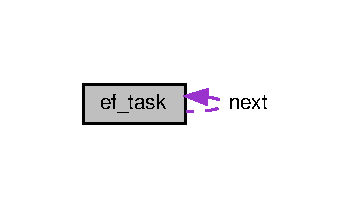
\includegraphics[width=169pt]{structef__task__coll__graph}
\end{center}
\end{figure}
\subsection*{Data Fields}
\begin{DoxyCompactItemize}
\item 
char($\ast$ \hyperlink{structef__task_a5e340b112e45de9d5398e316d7139115}{task} )()
\begin{DoxyCompactList}\small\item\em user defined task (in protothreads) \end{DoxyCompactList}\item 
struct \hyperlink{structef__task}{ef\+\_\+task} $\ast$ \hyperlink{structef__task_a7ca29f94c5801eeb742c458ab15cb9e4}{next}
\begin{DoxyCompactList}\small\item\em linked-\/list \end{DoxyCompactList}\end{DoxyCompactItemize}


\subsection{Detailed Description}
protothread task declaration 

\subsection{Field Documentation}
\mbox{\Hypertarget{structef__task_a5e340b112e45de9d5398e316d7139115}\label{structef__task_a5e340b112e45de9d5398e316d7139115}} 
\index{ef\+\_\+task@{ef\+\_\+task}!task@{task}}
\index{task@{task}!ef\+\_\+task@{ef\+\_\+task}}
\subsubsection{\texorpdfstring{task}{task}}
{\footnotesize\ttfamily char($\ast$ ef\+\_\+task\+::task) ()}



user defined task (in protothreads) 

\mbox{\Hypertarget{structef__task_a7ca29f94c5801eeb742c458ab15cb9e4}\label{structef__task_a7ca29f94c5801eeb742c458ab15cb9e4}} 
\index{ef\+\_\+task@{ef\+\_\+task}!next@{next}}
\index{next@{next}!ef\+\_\+task@{ef\+\_\+task}}
\subsubsection{\texorpdfstring{next}{next}}
{\footnotesize\ttfamily struct \hyperlink{structef__task}{ef\+\_\+task}$\ast$ ef\+\_\+task\+::next}



linked-\/list 



The documentation for this struct was generated from the following file\+:\begin{DoxyCompactItemize}
\item 
src/\hyperlink{eforth__core_8h}{eforth\+\_\+core.\+h}\end{DoxyCompactItemize}

\chapter{File Documentation}
\hypertarget{eforth1_8h}{}\doxysection{src/eforth1.h File Reference}
\label{eforth1_8h}\index{src/eforth1.h@{src/eforth1.h}}
{\ttfamily \#include $<$Arduino.\+h$>$}\newline
{\ttfamily \#include $<$time.\+h$>$}\newline
Include dependency graph for eforth1.\+h\+:
\nopagebreak
\begin{figure}[H]
\begin{center}
\leavevmode
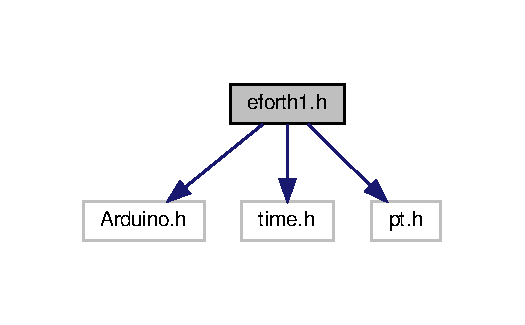
\includegraphics[width=210pt]{eforth1_8h__incl}
\end{center}
\end{figure}
\doxysubsection*{Functions}
\begin{DoxyCompactItemize}
\item 
void \mbox{\hyperlink{eforth1_8h_a3be4743e748619321c1a4f95928e8de1}{ef\+\_\+setup}} (Stream \&io\+\_\+stream=Serial)
\item 
void \mbox{\hyperlink{eforth1_8h_a1fb0d84284dc4203d4a4e4dbe8e07b29}{ef\+\_\+run}} ()
\end{DoxyCompactItemize}


\doxysubsection{Function Documentation}
\mbox{\Hypertarget{eforth1_8h_a3be4743e748619321c1a4f95928e8de1}\label{eforth1_8h_a3be4743e748619321c1a4f95928e8de1}} 
\index{eforth1.h@{eforth1.h}!ef\_setup@{ef\_setup}}
\index{ef\_setup@{ef\_setup}!eforth1.h@{eforth1.h}}
\doxysubsubsection{\texorpdfstring{ef\_setup()}{ef\_setup()}}
{\footnotesize\ttfamily void ef\+\_\+setup (\begin{DoxyParamCaption}\item[{Stream \&}]{io\+\_\+stream = {\ttfamily Serial} }\end{DoxyParamCaption})}

setup (called by Arduino setup) \mbox{\Hypertarget{eforth1_8h_a1fb0d84284dc4203d4a4e4dbe8e07b29}\label{eforth1_8h_a1fb0d84284dc4203d4a4e4dbe8e07b29}} 
\index{eforth1.h@{eforth1.h}!ef\_run@{ef\_run}}
\index{ef\_run@{ef\_run}!eforth1.h@{eforth1.h}}
\doxysubsubsection{\texorpdfstring{ef\_run()}{ef\_run()}}
{\footnotesize\ttfamily void ef\+\_\+run (\begin{DoxyParamCaption}{ }\end{DoxyParamCaption})}

single step e\+Forth virtual machine 
\hypertarget{eforth1_8ino}{}\doxysection{eforth1.\+ino File Reference}
\label{eforth1_8ino}\index{eforth1.ino@{eforth1.ino}}

\hypertarget{eforth__asm_8cpp}{}\doxysection{src/eforth\+\_\+asm.cpp File Reference}
\label{eforth__asm_8cpp}\index{src/eforth\_asm.cpp@{src/eforth\_asm.cpp}}


e\+Forth Assembler module  


{\ttfamily \#include \char`\"{}eforth\+\_\+core.\+h\char`\"{}}\newline
{\ttfamily \#include \char`\"{}eforth\+\_\+asm.\+h\char`\"{}}\newline
Include dependency graph for eforth\+\_\+asm.\+cpp\+:\nopagebreak
\begin{figure}[H]
\begin{center}
\leavevmode
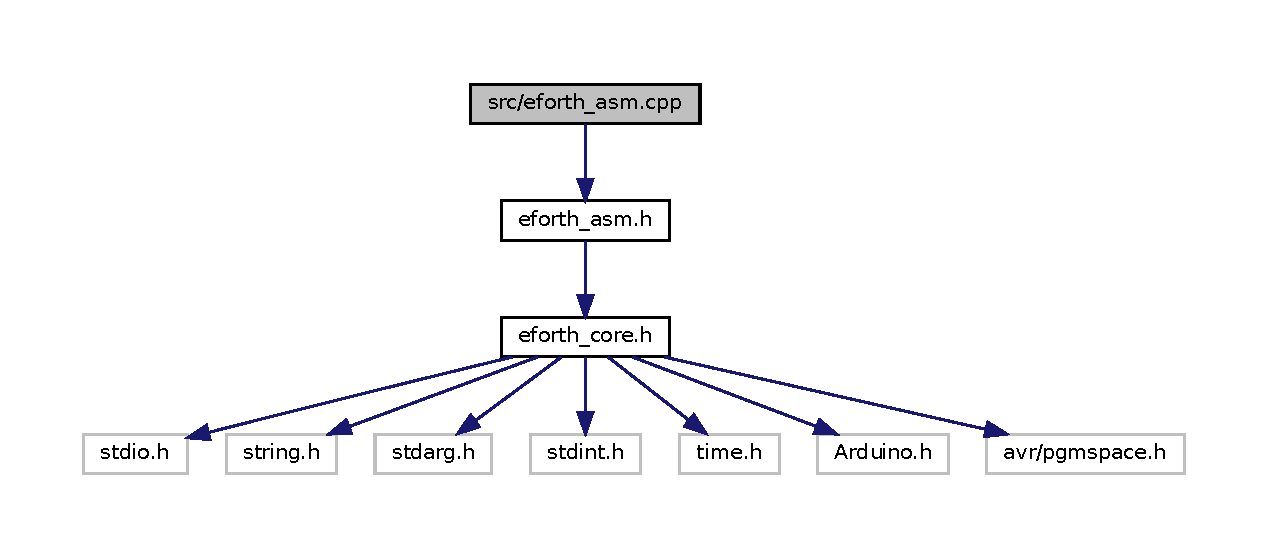
\includegraphics[width=350pt]{eforth__asm_8cpp__incl}
\end{center}
\end{figure}
\doxysubsection*{Namespaces}
\begin{DoxyCompactItemize}
\item 
 \mbox{\hyperlink{namespaceEfAsm}{Ef\+Asm}}
\end{DoxyCompactItemize}
\doxysubsection*{Macros}
\begin{DoxyCompactItemize}
\item 
\#define \mbox{\hyperlink{eforth__asm_8cpp_a9ea1e8dcf59129fa7bfe31bbc1f87d8e}{f\+C\+M\+PL}}~0x40
\item 
\#define \mbox{\hyperlink{eforth__asm_8cpp_a84054c8a0e922b86c0d99ea4cfdab34e}{f\+I\+M\+MD}}~0x80
\item 
\#define \mbox{\hyperlink{eforth__asm_8cpp_a27fcb44e39b3c4a0d37e34faab596803}{D\+U\+M\+P\+\_\+\+R\+O\+W\+\_\+\+W\+I\+D\+TH}}~0x40
\item 
\#define \mbox{\hyperlink{eforth__asm_8cpp_ac7635cecf944d5bfcc89665c08022828}{OP}}(name)~op\#\#name
\end{DoxyCompactItemize}
\doxysubsection*{Enumerations}
\begin{DoxyCompactItemize}
\item 
enum \{ \mbox{\hyperlink{eforth__asm_8cpp_a06fc87d81c62e9abb8790b6e5713c55ba40ca1718b18204c5206b1cdf98ddead4}{op\+N\+OP}} = 0, 
\mbox{\hyperlink{eforth__asm_8cpp_a06fc87d81c62e9abb8790b6e5713c55ba9985f02d910b285a8c65e383fb1b2f0d}{O\+P\+C\+O\+D\+ES}}
 \}
\end{DoxyCompactItemize}
\doxysubsection*{Functions}
\begin{DoxyCompactItemize}
\item 
int \mbox{\hyperlink{namespaceEfAsm_acc07308cd4b29f3582ea2045d3326915}{Ef\+Asm\+::assemble}} (\mbox{\hyperlink{eforth__core_8h_aa63ef7b996d5487ce35a5a66601f3e73}{U8}} $\ast$cdata)
\item 
void \mbox{\hyperlink{eforth__asm_8cpp_ac7b7418379a5743a1883314bfd9ee874}{\+\_\+dump\+\_\+rom}} (\mbox{\hyperlink{eforth__core_8h_aa63ef7b996d5487ce35a5a66601f3e73}{U8}} $\ast$cdata, int len)
\item 
int \mbox{\hyperlink{eforth__asm_8cpp_a94e10412bf5e1f89d12efb94e80979c8}{ef\+\_\+assemble}} (\mbox{\hyperlink{eforth__core_8h_aa63ef7b996d5487ce35a5a66601f3e73}{U8}} $\ast$cdata)
\end{DoxyCompactItemize}
\begin{Indent}\textbf{ Memory Dumpers}\par
\begin{DoxyCompactItemize}
\item 
void \mbox{\hyperlink{namespaceEfAsm_a3ff1e256bb2a99fdb6fee8b453e4361e}{Ef\+Asm\+::\+\_\+dump}} (int b, int u)
\item 
void \mbox{\hyperlink{namespaceEfAsm_a5bdea27a67eb879d5dd1b58bed56b9bd}{Ef\+Asm\+::\+\_\+rdump}} ()
\begin{DoxyCompactList}\small\item\em dump return stack \end{DoxyCompactList}\end{DoxyCompactItemize}
\end{Indent}
\begin{Indent}\textbf{ Assembler -\/ Word Creation Headers}\par
\begin{DoxyCompactItemize}
\item 
void \mbox{\hyperlink{namespaceEfAsm_a27da79e08a45cd4ad90cffc847a04280}{Ef\+Asm\+::\+\_\+header}} (int lex, F\+C\+H\+AR $\ast$seq)
\item 
int \mbox{\hyperlink{namespaceEfAsm_a7d79fdd3d59e237e0381d1798e2050bb}{Ef\+Asm\+::\+\_\+code}} (F\+C\+H\+AR $\ast$seg, int len,...)
\item 
int \mbox{\hyperlink{namespaceEfAsm_acce2eabb9a04fa5c08fc95932e2f92ae}{Ef\+Asm\+::\+\_\+colon}} (F\+C\+H\+AR $\ast$seg, int len,...)
\item 
int \mbox{\hyperlink{namespaceEfAsm_acb8719a8b6a78152c8676f735dc7c467}{Ef\+Asm\+::\+\_\+immed}} (F\+C\+H\+AR $\ast$seg, int len,...)
\item 
int \mbox{\hyperlink{namespaceEfAsm_abb1c9544549fc018a1ed1e8345cc66f3}{Ef\+Asm\+::\+\_\+label}} (int len,...)
\end{DoxyCompactItemize}
\end{Indent}
\begin{Indent}\textbf{ Assembler -\/ Branching Ops}\par
\begin{DoxyCompactItemize}
\item 
void \mbox{\hyperlink{namespaceEfAsm_ab18b552c595cf956387d2e4427384563}{Ef\+Asm\+::\+\_\+begin}} (int len,...)
\item 
void \mbox{\hyperlink{namespaceEfAsm_a5b6bf226f290864b6a596069e4a0cf74}{Ef\+Asm\+::\+\_\+while}} (int len,...)
\item 
void \mbox{\hyperlink{namespaceEfAsm_a3f42a6bd0929a03c700ace952e186997}{Ef\+Asm\+::\+\_\+repeat}} (int len,...)
\item 
void \mbox{\hyperlink{namespaceEfAsm_adcd97bc33014c89d91e19cc4a217b5e8}{Ef\+Asm\+::\+\_\+until}} (int len,...)
\item 
void \mbox{\hyperlink{namespaceEfAsm_ab7b5835572c00662317647be9a49b2b3}{Ef\+Asm\+::\+\_\+again}} (int len,...)
\item 
void \mbox{\hyperlink{namespaceEfAsm_a771a43815e0f65570de187ee456938e8}{Ef\+Asm\+::\+\_\+for}} (int len,...)
\item 
void \mbox{\hyperlink{namespaceEfAsm_abf110638d9dc2195b884957885128696}{Ef\+Asm\+::\+\_\+aft}} (int len,...)
\item 
void \mbox{\hyperlink{namespaceEfAsm_a2df77b2810440262c7ade5fc911f8c8a}{Ef\+Asm\+::\+\_\+nxt}} (int len,...)
\item 
void \mbox{\hyperlink{namespaceEfAsm_ab786d49b7cbf077b6a706a308167b5ce}{Ef\+Asm\+::\+\_\+if}} (int len,...)
\item 
void \mbox{\hyperlink{namespaceEfAsm_a8c4966a74388b9427ae2771419d73430}{Ef\+Asm\+::\+\_\+else}} (int len,...)
\item 
void \mbox{\hyperlink{namespaceEfAsm_a5a0ec1a59cc273ec7db9b5a2af2779ef}{Ef\+Asm\+::\+\_\+then}} (int len,...)
\end{DoxyCompactItemize}
\end{Indent}
\begin{Indent}\textbf{ Assembler -\/ IO Functions}\par
\begin{DoxyCompactItemize}
\item 
void \mbox{\hyperlink{namespaceEfAsm_afb006746d990ab51ca27545ab004f260}{Ef\+Asm\+::\+\_\+dotq}} (F\+C\+H\+AR $\ast$seq)
\item 
void \mbox{\hyperlink{namespaceEfAsm_a902f7d3df2665aef0f0aa00269bf932d}{Ef\+Asm\+::\+\_\+strq}} (F\+C\+H\+AR $\ast$seq)
\item 
void \mbox{\hyperlink{namespaceEfAsm_a4499c7338bdc153d5f19127e8a3d59a7}{Ef\+Asm\+::\+\_\+abortq}} (F\+C\+H\+AR $\ast$seq)
\end{DoxyCompactItemize}
\end{Indent}
\begin{Indent}\textbf{ Memory Dumpers}\par
\begin{DoxyCompactItemize}
\item 
void \mbox{\hyperlink{namespaceEfAsm_a3ff1e256bb2a99fdb6fee8b453e4361e}{Ef\+Asm\+::\+\_\+dump}} (int b, int u)
\item 
void \mbox{\hyperlink{namespaceEfAsm_a5bdea27a67eb879d5dd1b58bed56b9bd}{Ef\+Asm\+::\+\_\+rdump}} ()
\begin{DoxyCompactList}\small\item\em dump return stack \end{DoxyCompactList}\end{DoxyCompactItemize}
\end{Indent}
\begin{Indent}\textbf{ Assembler -\/ String/\+Byte Movers}\par
\begin{DoxyCompactItemize}
\item 
int \mbox{\hyperlink{namespaceEfAsm_a59af885d0e26e3c82059708948d2df37}{Ef\+Asm\+::\+\_\+strlen}} (F\+C\+H\+AR $\ast$seq)
\end{DoxyCompactItemize}
\end{Indent}
\begin{Indent}\textbf{ Assembler -\/ Word Creation Headers}\par
\begin{DoxyCompactItemize}
\item 
void \mbox{\hyperlink{namespaceEfAsm_a27da79e08a45cd4ad90cffc847a04280}{Ef\+Asm\+::\+\_\+header}} (int lex, F\+C\+H\+AR $\ast$seq)
\item 
int \mbox{\hyperlink{namespaceEfAsm_a7d79fdd3d59e237e0381d1798e2050bb}{Ef\+Asm\+::\+\_\+code}} (F\+C\+H\+AR $\ast$seg, int len,...)
\item 
int \mbox{\hyperlink{namespaceEfAsm_acce2eabb9a04fa5c08fc95932e2f92ae}{Ef\+Asm\+::\+\_\+colon}} (F\+C\+H\+AR $\ast$seg, int len,...)
\item 
int \mbox{\hyperlink{namespaceEfAsm_acb8719a8b6a78152c8676f735dc7c467}{Ef\+Asm\+::\+\_\+immed}} (F\+C\+H\+AR $\ast$seg, int len,...)
\item 
int \mbox{\hyperlink{namespaceEfAsm_abb1c9544549fc018a1ed1e8345cc66f3}{Ef\+Asm\+::\+\_\+label}} (int len,...)
\end{DoxyCompactItemize}
\end{Indent}
\begin{Indent}\textbf{ Assembler -\/ Branching Ops}\par
\begin{DoxyCompactItemize}
\item 
void \mbox{\hyperlink{namespaceEfAsm_ab18b552c595cf956387d2e4427384563}{Ef\+Asm\+::\+\_\+begin}} (int len,...)
\item 
void \mbox{\hyperlink{namespaceEfAsm_a5b6bf226f290864b6a596069e4a0cf74}{Ef\+Asm\+::\+\_\+while}} (int len,...)
\item 
void \mbox{\hyperlink{namespaceEfAsm_a3f42a6bd0929a03c700ace952e186997}{Ef\+Asm\+::\+\_\+repeat}} (int len,...)
\item 
void \mbox{\hyperlink{namespaceEfAsm_adcd97bc33014c89d91e19cc4a217b5e8}{Ef\+Asm\+::\+\_\+until}} (int len,...)
\item 
void \mbox{\hyperlink{namespaceEfAsm_ab7b5835572c00662317647be9a49b2b3}{Ef\+Asm\+::\+\_\+again}} (int len,...)
\item 
void \mbox{\hyperlink{namespaceEfAsm_a771a43815e0f65570de187ee456938e8}{Ef\+Asm\+::\+\_\+for}} (int len,...)
\item 
void \mbox{\hyperlink{namespaceEfAsm_abf110638d9dc2195b884957885128696}{Ef\+Asm\+::\+\_\+aft}} (int len,...)
\item 
void \mbox{\hyperlink{namespaceEfAsm_a2df77b2810440262c7ade5fc911f8c8a}{Ef\+Asm\+::\+\_\+nxt}} (int len,...)
\item 
void \mbox{\hyperlink{namespaceEfAsm_ab786d49b7cbf077b6a706a308167b5ce}{Ef\+Asm\+::\+\_\+if}} (int len,...)
\item 
void \mbox{\hyperlink{namespaceEfAsm_a8c4966a74388b9427ae2771419d73430}{Ef\+Asm\+::\+\_\+else}} (int len,...)
\item 
void \mbox{\hyperlink{namespaceEfAsm_a5a0ec1a59cc273ec7db9b5a2af2779ef}{Ef\+Asm\+::\+\_\+then}} (int len,...)
\end{DoxyCompactItemize}
\end{Indent}
\begin{Indent}\textbf{ Assembler -\/ IO Functions}\par
\begin{DoxyCompactItemize}
\item 
void \mbox{\hyperlink{namespaceEfAsm_afb006746d990ab51ca27545ab004f260}{Ef\+Asm\+::\+\_\+dotq}} (F\+C\+H\+AR $\ast$seq)
\item 
void \mbox{\hyperlink{namespaceEfAsm_a902f7d3df2665aef0f0aa00269bf932d}{Ef\+Asm\+::\+\_\+strq}} (F\+C\+H\+AR $\ast$seq)
\item 
void \mbox{\hyperlink{namespaceEfAsm_a4499c7338bdc153d5f19127e8a3d59a7}{Ef\+Asm\+::\+\_\+abortq}} (F\+C\+H\+AR $\ast$seq)
\end{DoxyCompactItemize}
\end{Indent}
\doxysubsection*{Variables}
\begin{Indent}\textbf{ Compiled Address for Branching}\par
\begin{DoxyCompactItemize}
\item 
\mbox{\hyperlink{eforth__core_8h_a5fd90490ca5b2ceb72bf8b2c89a9634b}{IU}} \mbox{\hyperlink{namespaceEfAsm_a441c683b38bd339236b4bd6e305750cd}{Ef\+Asm\+::\+B\+R\+AN}}
\item 
\mbox{\hyperlink{eforth__core_8h_a5fd90490ca5b2ceb72bf8b2c89a9634b}{IU}} \mbox{\hyperlink{namespaceEfAsm_a7b221cc855cf8ca6334d2c7cb5879542}{Ef\+Asm\+::\+Q\+B\+R\+AN}}
\item 
\mbox{\hyperlink{eforth__core_8h_a5fd90490ca5b2ceb72bf8b2c89a9634b}{IU}} \mbox{\hyperlink{namespaceEfAsm_a86b03a1e4d3a8b4c0cdfd8d9fc8f7010}{Ef\+Asm\+::\+D\+O\+N\+XT}}
\begin{DoxyCompactList}\small\item\em addr of branching ops, used by branching ops \end{DoxyCompactList}\item 
\mbox{\hyperlink{eforth__core_8h_a5fd90490ca5b2ceb72bf8b2c89a9634b}{IU}} \mbox{\hyperlink{namespaceEfAsm_a6b8f6e7e77a210d6bfaf73bb43897580}{Ef\+Asm\+::\+D\+O\+T\+QP}}
\item 
\mbox{\hyperlink{eforth__core_8h_a5fd90490ca5b2ceb72bf8b2c89a9634b}{IU}} \mbox{\hyperlink{namespaceEfAsm_ac31352a003705d9569ef3314d62342fb}{Ef\+Asm\+::\+S\+T\+R\+QP}}
\item 
\mbox{\hyperlink{eforth__core_8h_a5fd90490ca5b2ceb72bf8b2c89a9634b}{IU}} \mbox{\hyperlink{namespaceEfAsm_a13343dd66b80ba0cbe75877f7a6980d9}{Ef\+Asm\+::\+A\+B\+O\+R\+QP}}
\begin{DoxyCompactList}\small\item\em addr of output ops, used by \+\_\+dotq, \+\_\+strq, \+\_\+abortq \end{DoxyCompactList}\item 
\mbox{\hyperlink{eforth__core_8h_a5fd90490ca5b2ceb72bf8b2c89a9634b}{IU}} \mbox{\hyperlink{namespaceEfAsm_ab44525c5e6436fa71223dfb207741699}{Ef\+Asm\+::\+T\+OR}}
\begin{DoxyCompactList}\small\item\em addres of \char`\"{}$>$\+R\char`\"{} op, used by \+\_\+for \end{DoxyCompactList}\item 
\mbox{\hyperlink{eforth__core_8h_a5fd90490ca5b2ceb72bf8b2c89a9634b}{IU}} \mbox{\hyperlink{namespaceEfAsm_aa3dd7a4f331c954244daaddf0177f059}{Ef\+Asm\+::\+N\+OP}} = 0xffff
\begin{DoxyCompactList}\small\item\em N\+OP set to ffff to prevent access before initialized. \end{DoxyCompactList}\end{DoxyCompactItemize}
\end{Indent}
\begin{Indent}\textbf{ Return Stack for Branching Ops}\par
\begin{DoxyCompactItemize}
\item 
\mbox{\hyperlink{eforth__core_8h_aa63ef7b996d5487ce35a5a66601f3e73}{U8}} $\ast$ \mbox{\hyperlink{namespaceEfAsm_a1b5e7cec0310945601603be02b8f8834}{Ef\+Asm\+::\+Byte}}
\begin{DoxyCompactList}\small\item\em assembler byte array (heap) \end{DoxyCompactList}\item 
\mbox{\hyperlink{eforth__core_8h_aa63ef7b996d5487ce35a5a66601f3e73}{U8}} \mbox{\hyperlink{namespaceEfAsm_a85323f491b7b3ea3883bad0c91d9de17}{Ef\+Asm\+::R}}
\begin{DoxyCompactList}\small\item\em assembler return stack index \end{DoxyCompactList}\item 
\mbox{\hyperlink{eforth__core_8h_a5fd90490ca5b2ceb72bf8b2c89a9634b}{IU}} \mbox{\hyperlink{namespaceEfAsm_a77406fd9edef6925ff2bafc8746085eb}{Ef\+Asm\+::\+PC}}
\begin{DoxyCompactList}\small\item\em assembler program counter \end{DoxyCompactList}\item 
\mbox{\hyperlink{eforth__core_8h_a5fd90490ca5b2ceb72bf8b2c89a9634b}{IU}} \mbox{\hyperlink{namespaceEfAsm_a5bc71a8752683bc40a6f206bf3585d0f}{Ef\+Asm\+::\+Link}}
\begin{DoxyCompactList}\small\item\em link to previous word \end{DoxyCompactList}\end{DoxyCompactItemize}
\end{Indent}
\begin{Indent}\textbf{ Compiled Address for Branching}\par
\begin{DoxyCompactItemize}
\item 
\mbox{\hyperlink{eforth__core_8h_a5fd90490ca5b2ceb72bf8b2c89a9634b}{IU}} \mbox{\hyperlink{namespaceEfAsm_a441c683b38bd339236b4bd6e305750cd}{Ef\+Asm\+::\+B\+R\+AN}}
\item 
\mbox{\hyperlink{eforth__core_8h_a5fd90490ca5b2ceb72bf8b2c89a9634b}{IU}} \mbox{\hyperlink{namespaceEfAsm_a7b221cc855cf8ca6334d2c7cb5879542}{Ef\+Asm\+::\+Q\+B\+R\+AN}}
\item 
\mbox{\hyperlink{eforth__core_8h_a5fd90490ca5b2ceb72bf8b2c89a9634b}{IU}} \mbox{\hyperlink{namespaceEfAsm_a86b03a1e4d3a8b4c0cdfd8d9fc8f7010}{Ef\+Asm\+::\+D\+O\+N\+XT}}
\begin{DoxyCompactList}\small\item\em addr of branching ops, used by branching ops \end{DoxyCompactList}\item 
\mbox{\hyperlink{eforth__core_8h_a5fd90490ca5b2ceb72bf8b2c89a9634b}{IU}} \mbox{\hyperlink{namespaceEfAsm_a6b8f6e7e77a210d6bfaf73bb43897580}{Ef\+Asm\+::\+D\+O\+T\+QP}}
\item 
\mbox{\hyperlink{eforth__core_8h_a5fd90490ca5b2ceb72bf8b2c89a9634b}{IU}} \mbox{\hyperlink{namespaceEfAsm_ac31352a003705d9569ef3314d62342fb}{Ef\+Asm\+::\+S\+T\+R\+QP}}
\item 
\mbox{\hyperlink{eforth__core_8h_a5fd90490ca5b2ceb72bf8b2c89a9634b}{IU}} \mbox{\hyperlink{namespaceEfAsm_a13343dd66b80ba0cbe75877f7a6980d9}{Ef\+Asm\+::\+A\+B\+O\+R\+QP}}
\begin{DoxyCompactList}\small\item\em addr of output ops, used by \+\_\+dotq, \+\_\+strq, \+\_\+abortq \end{DoxyCompactList}\item 
\mbox{\hyperlink{eforth__core_8h_a5fd90490ca5b2ceb72bf8b2c89a9634b}{IU}} \mbox{\hyperlink{namespaceEfAsm_ab44525c5e6436fa71223dfb207741699}{Ef\+Asm\+::\+T\+OR}}
\begin{DoxyCompactList}\small\item\em addres of \char`\"{}$>$\+R\char`\"{} op, used by \+\_\+for \end{DoxyCompactList}\item 
\mbox{\hyperlink{eforth__core_8h_a5fd90490ca5b2ceb72bf8b2c89a9634b}{IU}} \mbox{\hyperlink{namespaceEfAsm_aa3dd7a4f331c954244daaddf0177f059}{Ef\+Asm\+::\+N\+OP}} = 0xffff
\begin{DoxyCompactList}\small\item\em N\+OP set to ffff to prevent access before initialized. \end{DoxyCompactList}\end{DoxyCompactItemize}
\end{Indent}
\begin{Indent}\textbf{ Return Stack for Branching Ops}\par
\begin{DoxyCompactItemize}
\item 
\mbox{\hyperlink{eforth__core_8h_aa63ef7b996d5487ce35a5a66601f3e73}{U8}} $\ast$ \mbox{\hyperlink{namespaceEfAsm_a1b5e7cec0310945601603be02b8f8834}{Ef\+Asm\+::\+Byte}}
\begin{DoxyCompactList}\small\item\em assembler byte array (heap) \end{DoxyCompactList}\item 
\mbox{\hyperlink{eforth__core_8h_aa63ef7b996d5487ce35a5a66601f3e73}{U8}} \mbox{\hyperlink{namespaceEfAsm_a85323f491b7b3ea3883bad0c91d9de17}{Ef\+Asm\+::R}}
\begin{DoxyCompactList}\small\item\em assembler return stack index \end{DoxyCompactList}\item 
\mbox{\hyperlink{eforth__core_8h_a5fd90490ca5b2ceb72bf8b2c89a9634b}{IU}} \mbox{\hyperlink{namespaceEfAsm_a77406fd9edef6925ff2bafc8746085eb}{Ef\+Asm\+::\+PC}}
\begin{DoxyCompactList}\small\item\em assembler program counter \end{DoxyCompactList}\item 
\mbox{\hyperlink{eforth__core_8h_a5fd90490ca5b2ceb72bf8b2c89a9634b}{IU}} \mbox{\hyperlink{namespaceEfAsm_a5bc71a8752683bc40a6f206bf3585d0f}{Ef\+Asm\+::\+Link}}
\begin{DoxyCompactList}\small\item\em link to previous word \end{DoxyCompactList}\end{DoxyCompactItemize}
\end{Indent}
\doxysubsection*{Assembler -\/ String/\+Byte Movers}
\begin{DoxyCompactItemize}
\item 
\#define \mbox{\hyperlink{eforth__asm_8cpp_a60ef63ffe304267efee1dd841faf4751}{C\+E\+L\+L\+C\+PY}}(n)
\item 
\#define \mbox{\hyperlink{eforth__asm_8cpp_abee5cbd8a5640f4b067cdc048b4c21ca}{P\+G\+M\+C\+PY}}(len,  seq)
\item 
\#define \mbox{\hyperlink{eforth__asm_8cpp_a49723d0c3f14a2ff23c8518ca5730fb0}{O\+P\+S\+TR}}(op,  seq)
\item 
int \mbox{\hyperlink{namespaceEfAsm_a59af885d0e26e3c82059708948d2df37}{Ef\+Asm\+::\+\_\+strlen}} (F\+C\+H\+AR $\ast$seq)
\end{DoxyCompactItemize}


\doxysubsection{Detailed Description}
e\+Forth Assembler module 

Forth Macro Assembler 

\doxysubsection{Macro Definition Documentation}
\mbox{\Hypertarget{eforth__asm_8cpp_a9ea1e8dcf59129fa7bfe31bbc1f87d8e}\label{eforth__asm_8cpp_a9ea1e8dcf59129fa7bfe31bbc1f87d8e}} 
\index{eforth\_asm.cpp@{eforth\_asm.cpp}!fCMPL@{fCMPL}}
\index{fCMPL@{fCMPL}!eforth\_asm.cpp@{eforth\_asm.cpp}}
\doxysubsubsection{\texorpdfstring{fCMPL}{fCMPL}}
{\footnotesize\ttfamily \#define f\+C\+M\+PL~0x40}

compile only flag \mbox{\Hypertarget{eforth__asm_8cpp_a84054c8a0e922b86c0d99ea4cfdab34e}\label{eforth__asm_8cpp_a84054c8a0e922b86c0d99ea4cfdab34e}} 
\index{eforth\_asm.cpp@{eforth\_asm.cpp}!fIMMD@{fIMMD}}
\index{fIMMD@{fIMMD}!eforth\_asm.cpp@{eforth\_asm.cpp}}
\doxysubsubsection{\texorpdfstring{fIMMD}{fIMMD}}
{\footnotesize\ttfamily \#define f\+I\+M\+MD~0x80}

immediate flag ~\newline
 \mbox{\Hypertarget{eforth__asm_8cpp_a27fcb44e39b3c4a0d37e34faab596803}\label{eforth__asm_8cpp_a27fcb44e39b3c4a0d37e34faab596803}} 
\index{eforth\_asm.cpp@{eforth\_asm.cpp}!DUMP\_ROW\_WIDTH@{DUMP\_ROW\_WIDTH}}
\index{DUMP\_ROW\_WIDTH@{DUMP\_ROW\_WIDTH}!eforth\_asm.cpp@{eforth\_asm.cpp}}
\doxysubsubsection{\texorpdfstring{DUMP\_ROW\_WIDTH}{DUMP\_ROW\_WIDTH}}
{\footnotesize\ttfamily \#define D\+U\+M\+P\+\_\+\+R\+O\+W\+\_\+\+W\+I\+D\+TH~0x40}

\mbox{\Hypertarget{eforth__asm_8cpp_ac7635cecf944d5bfcc89665c08022828}\label{eforth__asm_8cpp_ac7635cecf944d5bfcc89665c08022828}} 
\index{eforth\_asm.cpp@{eforth\_asm.cpp}!OP@{OP}}
\index{OP@{OP}!eforth\_asm.cpp@{eforth\_asm.cpp}}
\doxysubsubsection{\texorpdfstring{OP}{OP}}
{\footnotesize\ttfamily \#define OP(\begin{DoxyParamCaption}\item[{}]{name }\end{DoxyParamCaption})~op\#\#name}

define opcode enums Note\+: in sync with VM\textquotesingle{}s vtable \mbox{\Hypertarget{eforth__asm_8cpp_a60ef63ffe304267efee1dd841faf4751}\label{eforth__asm_8cpp_a60ef63ffe304267efee1dd841faf4751}} 
\index{eforth\_asm.cpp@{eforth\_asm.cpp}!CELLCPY@{CELLCPY}}
\index{CELLCPY@{CELLCPY}!eforth\_asm.cpp@{eforth\_asm.cpp}}
\doxysubsubsection{\texorpdfstring{CELLCPY}{CELLCPY}}
{\footnotesize\ttfamily \#define C\+E\+L\+L\+C\+PY(\begin{DoxyParamCaption}\item[{}]{n }\end{DoxyParamCaption})}

{\bfseries Value\+:}
\begin{DoxyCode}{0}
\DoxyCodeLine{    \{                            \(\backslash\)}
\DoxyCodeLine{    va\_list argList;                            \(\backslash\)}
\DoxyCodeLine{    va\_start(argList, n);                       \(\backslash\)}
\DoxyCodeLine{    for (; n; n-\/-\/) \{                            \(\backslash\)}
\DoxyCodeLine{        IU j = (\mbox{\hyperlink{eforth__core_8h_a5fd90490ca5b2ceb72bf8b2c89a9634b}{IU}})va\_arg(argList, \textcolor{keywordtype}{int});        \(\backslash\)}
\DoxyCodeLine{        if (j==\mbox{\hyperlink{namespaceEfAsm_aa3dd7a4f331c954244daaddf0177f059}{NOP}}) \textcolor{keywordflow}{continue};                   \(\backslash\)}
\DoxyCodeLine{        STORE(j);                               \(\backslash\)}
\DoxyCodeLine{        DEBUG(\textcolor{stringliteral}{" \%04x"}, j);                      \(\backslash\)}
\DoxyCodeLine{    \}                                           \(\backslash\)}
\DoxyCodeLine{    va\_end(argList);                            \(\backslash\)}
\DoxyCodeLine{    \_rdump();                                   \(\backslash\)}
\DoxyCodeLine{\}}

\end{DoxyCode}
\mbox{\Hypertarget{eforth__asm_8cpp_abee5cbd8a5640f4b067cdc048b4c21ca}\label{eforth__asm_8cpp_abee5cbd8a5640f4b067cdc048b4c21ca}} 
\index{eforth\_asm.cpp@{eforth\_asm.cpp}!PGMCPY@{PGMCPY}}
\index{PGMCPY@{PGMCPY}!eforth\_asm.cpp@{eforth\_asm.cpp}}
\doxysubsubsection{\texorpdfstring{PGMCPY}{PGMCPY}}
{\footnotesize\ttfamily \#define P\+G\+M\+C\+PY(\begin{DoxyParamCaption}\item[{}]{len,  }\item[{}]{seq }\end{DoxyParamCaption})}

{\bfseries Value\+:}
\begin{DoxyCode}{0}
\DoxyCodeLine{    \{                      \(\backslash\)}
\DoxyCodeLine{    PGM\_P p = \textcolor{keyword}{reinterpret\_cast<}PGM\_P\textcolor{keyword}{>}(seq);     \(\backslash\)}
\DoxyCodeLine{    for (\textcolor{keywordtype}{int} i=0; i < len; i++) \{               \(\backslash\)}
\DoxyCodeLine{        BSET(\mbox{\hyperlink{namespaceEfAsm_a77406fd9edef6925ff2bafc8746085eb}{PC}}++, pgm\_read\_byte(p++));         \(\backslash\)}
\DoxyCodeLine{    \}                                           \(\backslash\)}
\DoxyCodeLine{\}}

\end{DoxyCode}
\mbox{\Hypertarget{eforth__asm_8cpp_a49723d0c3f14a2ff23c8518ca5730fb0}\label{eforth__asm_8cpp_a49723d0c3f14a2ff23c8518ca5730fb0}} 
\index{eforth\_asm.cpp@{eforth\_asm.cpp}!OPSTR@{OPSTR}}
\index{OPSTR@{OPSTR}!eforth\_asm.cpp@{eforth\_asm.cpp}}
\doxysubsubsection{\texorpdfstring{OPSTR}{OPSTR}}
{\footnotesize\ttfamily \#define O\+P\+S\+TR(\begin{DoxyParamCaption}\item[{}]{op,  }\item[{}]{seq }\end{DoxyParamCaption})}

{\bfseries Value\+:}
\begin{DoxyCode}{0}
\DoxyCodeLine{    \{                        \(\backslash\)}
\DoxyCodeLine{    STORE(op);                                  \(\backslash\)}
\DoxyCodeLine{    int len = \mbox{\hyperlink{namespaceEfAsm_a59af885d0e26e3c82059708948d2df37}{\_strlen}}(seq);                     \(\backslash\)}
\DoxyCodeLine{    BSET(\mbox{\hyperlink{namespaceEfAsm_a77406fd9edef6925ff2bafc8746085eb}{PC}}++, len);                            \(\backslash\)}
\DoxyCodeLine{    PGMCPY(len, seq);                           \(\backslash\)}
\DoxyCodeLine{\}}

\end{DoxyCode}


\doxysubsection{Enumeration Type Documentation}
\mbox{\Hypertarget{eforth__asm_8cpp_a06fc87d81c62e9abb8790b6e5713c55b}\label{eforth__asm_8cpp_a06fc87d81c62e9abb8790b6e5713c55b}} 
\doxysubsubsection{\texorpdfstring{anonymous enum}{anonymous enum}}
{\footnotesize\ttfamily anonymous enum}

\begin{DoxyEnumFields}{Enumerator}
\raisebox{\heightof{T}}[0pt][0pt]{\index{opNOP@{opNOP}!eforth\_asm.cpp@{eforth\_asm.cpp}}\index{eforth\_asm.cpp@{eforth\_asm.cpp}!opNOP@{opNOP}}}\mbox{\Hypertarget{eforth__asm_8cpp_a06fc87d81c62e9abb8790b6e5713c55ba40ca1718b18204c5206b1cdf98ddead4}\label{eforth__asm_8cpp_a06fc87d81c62e9abb8790b6e5713c55ba40ca1718b18204c5206b1cdf98ddead4}} 
op\+N\+OP&opcodes start at 0 \\
\hline

\raisebox{\heightof{T}}[0pt][0pt]{\index{OPCODES@{OPCODES}!eforth\_asm.cpp@{eforth\_asm.cpp}}\index{eforth\_asm.cpp@{eforth\_asm.cpp}!OPCODES@{OPCODES}}}\mbox{\Hypertarget{eforth__asm_8cpp_a06fc87d81c62e9abb8790b6e5713c55ba9985f02d910b285a8c65e383fb1b2f0d}\label{eforth__asm_8cpp_a06fc87d81c62e9abb8790b6e5713c55ba9985f02d910b285a8c65e383fb1b2f0d}} 
O\+P\+C\+O\+D\+ES&\\
\hline

\end{DoxyEnumFields}


\doxysubsection{Function Documentation}
\mbox{\Hypertarget{eforth__asm_8cpp_ac7b7418379a5743a1883314bfd9ee874}\label{eforth__asm_8cpp_ac7b7418379a5743a1883314bfd9ee874}} 
\index{eforth\_asm.cpp@{eforth\_asm.cpp}!\_dump\_rom@{\_dump\_rom}}
\index{\_dump\_rom@{\_dump\_rom}!eforth\_asm.cpp@{eforth\_asm.cpp}}
\doxysubsubsection{\texorpdfstring{\_dump\_rom()}{\_dump\_rom()}}
{\footnotesize\ttfamily void \+\_\+dump\+\_\+rom (\begin{DoxyParamCaption}\item[{\mbox{\hyperlink{eforth__core_8h_aa63ef7b996d5487ce35a5a66601f3e73}{U8}} $\ast$}]{cdata,  }\item[{int}]{len }\end{DoxyParamCaption})}

create C array dump for R\+OM \mbox{\Hypertarget{eforth__asm_8cpp_a94e10412bf5e1f89d12efb94e80979c8}\label{eforth__asm_8cpp_a94e10412bf5e1f89d12efb94e80979c8}} 
\index{eforth\_asm.cpp@{eforth\_asm.cpp}!ef\_assemble@{ef\_assemble}}
\index{ef\_assemble@{ef\_assemble}!eforth\_asm.cpp@{eforth\_asm.cpp}}
\doxysubsubsection{\texorpdfstring{ef\_assemble()}{ef\_assemble()}}
{\footnotesize\ttfamily int ef\+\_\+assemble (\begin{DoxyParamCaption}\item[{\mbox{\hyperlink{eforth__core_8h_aa63ef7b996d5487ce35a5a66601f3e73}{U8}} $\ast$}]{cdata }\end{DoxyParamCaption})}


\hypertarget{eforth__asm_8h}{}\doxysection{src/eforth\+\_\+asm.h File Reference}
\label{eforth__asm_8h}\index{src/eforth\_asm.h@{src/eforth\_asm.h}}


e\+Forth assembler module header  


{\ttfamily \#include \char`\"{}eforth\+\_\+core.\+h\char`\"{}}\newline
Include dependency graph for eforth\+\_\+asm.\+h\+:\nopagebreak
\begin{figure}[H]
\begin{center}
\leavevmode
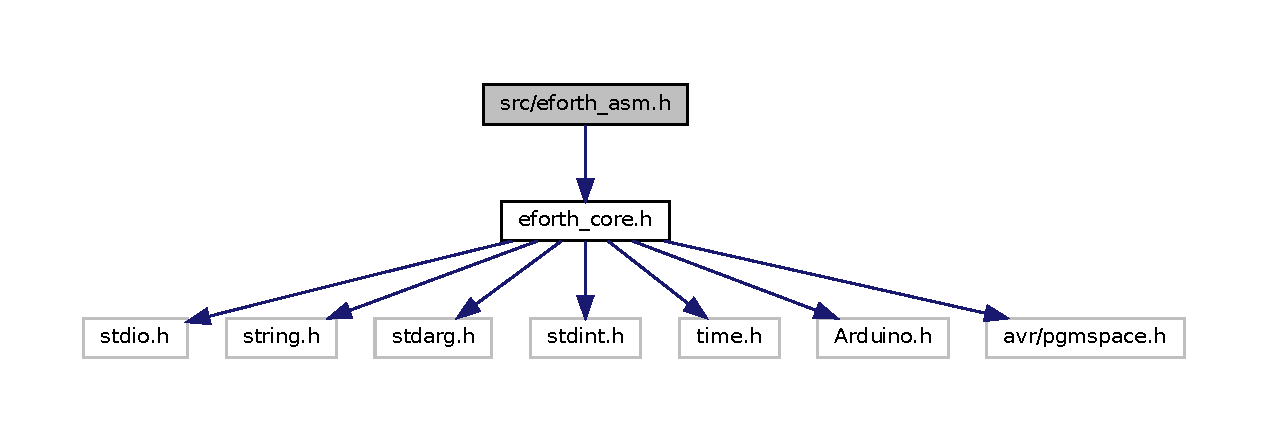
\includegraphics[width=350pt]{eforth__asm_8h__incl}
\end{center}
\end{figure}
This graph shows which files directly or indirectly include this file\+:\nopagebreak
\begin{figure}[H]
\begin{center}
\leavevmode
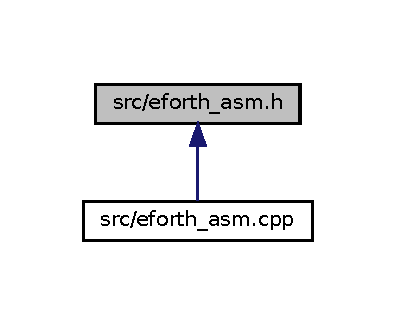
\includegraphics[width=190pt]{eforth__asm_8h__dep__incl}
\end{center}
\end{figure}
\doxysubsection*{Namespaces}
\begin{DoxyCompactItemize}
\item 
 \mbox{\hyperlink{namespaceEfAsm}{Ef\+Asm}}
\end{DoxyCompactItemize}
\doxysubsection*{Macros}
\begin{DoxyCompactItemize}
\item 
\#define \mbox{\hyperlink{eforth__asm_8h_a9ea1e8dcf59129fa7bfe31bbc1f87d8e}{f\+C\+M\+PL}}~0x40
\item 
\#define \mbox{\hyperlink{eforth__asm_8h_a84054c8a0e922b86c0d99ea4cfdab34e}{f\+I\+M\+MD}}~0x80
\item 
\#define \mbox{\hyperlink{eforth__asm_8h_ac7635cecf944d5bfcc89665c08022828}{OP}}(name)~op\#\#name
\item 
\#define \mbox{\hyperlink{eforth__asm_8h_a3254550e1d6d185f6b3e69b2d6468343}{D\+E\+B\+UG}}(s,  v)
\item 
\#define \mbox{\hyperlink{eforth__asm_8h_a49fac1253499dd76c037d22a8b7bcadf}{S\+H\+O\+W\+OP}}(op)
\item 
\#define \mbox{\hyperlink{eforth__asm_8h_a3041e6b675661edeec3883dd37d305af}{\+\_\+\+A\+R\+G\+\_\+N}}( \+\_\+1,  \+\_\+2,  \+\_\+3,  \+\_\+4,  \+\_\+5,  \+\_\+6,  \+\_\+7,  \+\_\+8,  \+\_\+9,  \+\_\+10,  \+\_\+11,  \+\_\+12,  \+\_\+13,  \+\_\+14,  \+\_\+15,  \+\_\+16,  \+\_\+17,  \+\_\+18,  \+\_\+19,  \+\_\+20,  \+\_\+21,  \+\_\+22,  \+\_\+23,  \+\_\+24,  \+\_\+25,  \+\_\+26,  \+\_\+27,  \+\_\+28,  \+\_\+29,  \+\_\+30,  \+\_\+31,  \+\_\+32,  \+\_\+33,  \+\_\+34,  \+\_\+35,  \+\_\+36,  \+\_\+37,  \+\_\+38,  \+\_\+39,  \+\_\+40,  \+\_\+41,  \+\_\+42,  \+\_\+43,  \+\_\+44,  \+\_\+45,  \+\_\+46,  \+\_\+47,  \+\_\+48,  \+\_\+49,  \+\_\+50,  \+\_\+51,  \+\_\+52,  \+\_\+53,  \+\_\+54,  \+\_\+55,  \+\_\+56,  \+\_\+57,  \+\_\+58,  \+\_\+59,  \+\_\+60,  \+\_\+61,  \+\_\+62,  \+\_\+63,  N, ...)~N
\item 
\#define \mbox{\hyperlink{eforth__asm_8h_a9b89373d972926a84265fdbd351494f1}{\+\_\+\+N\+U\+M\+\_\+N}}()
\item 
\#define \mbox{\hyperlink{eforth__asm_8h_a201f9ddd85daf92a29792435bb50d5bc}{\+\_\+\+N\+A\+R\+G0}}(...)~\mbox{\hyperlink{eforth__asm_8h_a3041e6b675661edeec3883dd37d305af}{\+\_\+\+A\+R\+G\+\_\+N}}(\+\_\+\+\_\+\+V\+A\+\_\+\+A\+R\+G\+S\+\_\+\+\_\+)
\item 
\#define \mbox{\hyperlink{eforth__asm_8h_a8b4fbd083a242445cf8eba9028c2a715}{\+\_\+\+N\+A\+RG}}(...)~\mbox{\hyperlink{eforth__asm_8h_a201f9ddd85daf92a29792435bb50d5bc}{\+\_\+\+N\+A\+R\+G0}}(\+\_\+, \#\#\+\_\+\+\_\+\+V\+A\+\_\+\+A\+R\+G\+S\+\_\+\+\_\+, \mbox{\hyperlink{eforth__asm_8h_a9b89373d972926a84265fdbd351494f1}{\+\_\+\+N\+U\+M\+\_\+N}}())
\item 
\#define \mbox{\hyperlink{group__Memory_ga60ef63ffe304267efee1dd841faf4751}{C\+E\+L\+L\+C\+PY}}(n)
\item 
\#define \mbox{\hyperlink{group__Memory_gabee5cbd8a5640f4b067cdc048b4c21ca}{P\+G\+M\+C\+PY}}(len,  seq)
\item 
\#define \mbox{\hyperlink{group__Memory_gaadf5c864c0d562a2efb56cdee5f3f206}{O\+P\+S\+TR}}(ip,  seq)
\end{DoxyCompactItemize}
\begin{Indent}\textbf{ Vargs Header (calculate number of parameters by compiler)}\par
\begin{DoxyCompactItemize}
\item 
\#define \mbox{\hyperlink{eforth__asm_8h_a6fd020b4ee926c9d86260e283bd2b660}{\+\_\+\+C\+O\+DE}}(seg, ...)~\+\_\+code(F(seg), \mbox{\hyperlink{eforth__asm_8h_a8b4fbd083a242445cf8eba9028c2a715}{\+\_\+\+N\+A\+RG}}(\+\_\+\+\_\+\+V\+A\+\_\+\+A\+R\+G\+S\+\_\+\+\_\+), \+\_\+\+\_\+\+V\+A\+\_\+\+A\+R\+G\+S\+\_\+\+\_\+)
\item 
\#define \mbox{\hyperlink{eforth__asm_8h_abeb04659d0496ec73bb428a13ea3e0b3}{\+\_\+\+X\+C\+O\+DE}}(seg,  x)~op\#\#x; \mbox{\hyperlink{eforth__asm_8h_a6fd020b4ee926c9d86260e283bd2b660}{\+\_\+\+C\+O\+DE}}(seg, op\#\#x, op\+E\+X\+IT)
\item 
\#define \mbox{\hyperlink{eforth__asm_8h_a9b4d0c68e95ce57cf7cdda4ee95d93f8}{\+\_\+\+C\+O\+L\+ON}}(seg, ...)~\+\_\+colon(F(seg), \mbox{\hyperlink{eforth__asm_8h_a8b4fbd083a242445cf8eba9028c2a715}{\+\_\+\+N\+A\+RG}}(\+\_\+\+\_\+\+V\+A\+\_\+\+A\+R\+G\+S\+\_\+\+\_\+), \+\_\+\+\_\+\+V\+A\+\_\+\+A\+R\+G\+S\+\_\+\+\_\+)
\item 
\#define \mbox{\hyperlink{eforth__asm_8h_a25550183c2dd8e46c4c93bc9b138ce87}{\+\_\+\+I\+M\+M\+ED}}(seg, ...)~\+\_\+immed(F(seg), \mbox{\hyperlink{eforth__asm_8h_a8b4fbd083a242445cf8eba9028c2a715}{\+\_\+\+N\+A\+RG}}(\+\_\+\+\_\+\+V\+A\+\_\+\+A\+R\+G\+S\+\_\+\+\_\+), \+\_\+\+\_\+\+V\+A\+\_\+\+A\+R\+G\+S\+\_\+\+\_\+)
\item 
\#define \mbox{\hyperlink{eforth__asm_8h_a59c00f3ec4f7443bcea73eb05cbd8642}{\+\_\+\+L\+A\+B\+EL}}(...)~\+\_\+label(\mbox{\hyperlink{eforth__asm_8h_a8b4fbd083a242445cf8eba9028c2a715}{\+\_\+\+N\+A\+RG}}(\+\_\+\+\_\+\+V\+A\+\_\+\+A\+R\+G\+S\+\_\+\+\_\+), \+\_\+\+\_\+\+V\+A\+\_\+\+A\+R\+G\+S\+\_\+\+\_\+)
\end{DoxyCompactItemize}
\end{Indent}
\begin{Indent}\textbf{ Vargs Branching}\par
\begin{DoxyCompactItemize}
\item 
\#define \mbox{\hyperlink{eforth__asm_8h_a56a32aefd52992d9ba072332da005f40}{\+\_\+\+B\+E\+G\+IN}}(...)~\+\_\+begin(\mbox{\hyperlink{eforth__asm_8h_a8b4fbd083a242445cf8eba9028c2a715}{\+\_\+\+N\+A\+RG}}(\+\_\+\+\_\+\+V\+A\+\_\+\+A\+R\+G\+S\+\_\+\+\_\+), \+\_\+\+\_\+\+V\+A\+\_\+\+A\+R\+G\+S\+\_\+\+\_\+)
\item 
\#define \mbox{\hyperlink{eforth__asm_8h_adac5ccc950018a5b7640be2555130ed1}{\+\_\+\+A\+G\+A\+IN}}(...)~\+\_\+again(\mbox{\hyperlink{eforth__asm_8h_a8b4fbd083a242445cf8eba9028c2a715}{\+\_\+\+N\+A\+RG}}(\+\_\+\+\_\+\+V\+A\+\_\+\+A\+R\+G\+S\+\_\+\+\_\+), \+\_\+\+\_\+\+V\+A\+\_\+\+A\+R\+G\+S\+\_\+\+\_\+)
\item 
\#define \mbox{\hyperlink{eforth__asm_8h_a412c374b83a229d1847514ae4357d2eb}{\+\_\+\+U\+N\+T\+IL}}(...)~\+\_\+until(\mbox{\hyperlink{eforth__asm_8h_a8b4fbd083a242445cf8eba9028c2a715}{\+\_\+\+N\+A\+RG}}(\+\_\+\+\_\+\+V\+A\+\_\+\+A\+R\+G\+S\+\_\+\+\_\+), \+\_\+\+\_\+\+V\+A\+\_\+\+A\+R\+G\+S\+\_\+\+\_\+)
\item 
\#define \mbox{\hyperlink{eforth__asm_8h_a62d262c8463829239eced86cde1509fe}{\+\_\+\+W\+H\+I\+LE}}(...)~\+\_\+while(\mbox{\hyperlink{eforth__asm_8h_a8b4fbd083a242445cf8eba9028c2a715}{\+\_\+\+N\+A\+RG}}(\+\_\+\+\_\+\+V\+A\+\_\+\+A\+R\+G\+S\+\_\+\+\_\+), \+\_\+\+\_\+\+V\+A\+\_\+\+A\+R\+G\+S\+\_\+\+\_\+)
\item 
\#define \mbox{\hyperlink{eforth__asm_8h_aa097837892926711dc5e7ca3b9d44d28}{\+\_\+\+R\+E\+P\+E\+AT}}(...)~\+\_\+repeat(\mbox{\hyperlink{eforth__asm_8h_a8b4fbd083a242445cf8eba9028c2a715}{\+\_\+\+N\+A\+RG}}(\+\_\+\+\_\+\+V\+A\+\_\+\+A\+R\+G\+S\+\_\+\+\_\+), \+\_\+\+\_\+\+V\+A\+\_\+\+A\+R\+G\+S\+\_\+\+\_\+)
\item 
\#define \mbox{\hyperlink{eforth__asm_8h_a6c2dc52d2057761fa4d361ec54d2dd90}{\+\_\+\+IF}}(...)~\+\_\+if(\mbox{\hyperlink{eforth__asm_8h_a8b4fbd083a242445cf8eba9028c2a715}{\+\_\+\+N\+A\+RG}}(\+\_\+\+\_\+\+V\+A\+\_\+\+A\+R\+G\+S\+\_\+\+\_\+), \+\_\+\+\_\+\+V\+A\+\_\+\+A\+R\+G\+S\+\_\+\+\_\+)
\item 
\#define \mbox{\hyperlink{eforth__asm_8h_a3fc480ce4c64cc8f0f7814e857083f9f}{\+\_\+\+E\+L\+SE}}(...)~\+\_\+else(\mbox{\hyperlink{eforth__asm_8h_a8b4fbd083a242445cf8eba9028c2a715}{\+\_\+\+N\+A\+RG}}(\+\_\+\+\_\+\+V\+A\+\_\+\+A\+R\+G\+S\+\_\+\+\_\+), \+\_\+\+\_\+\+V\+A\+\_\+\+A\+R\+G\+S\+\_\+\+\_\+)
\item 
\#define \mbox{\hyperlink{eforth__asm_8h_a0190db000e4d2486962e26b5fd8454eb}{\+\_\+\+T\+H\+EN}}(...)~\+\_\+then(\mbox{\hyperlink{eforth__asm_8h_a8b4fbd083a242445cf8eba9028c2a715}{\+\_\+\+N\+A\+RG}}(\+\_\+\+\_\+\+V\+A\+\_\+\+A\+R\+G\+S\+\_\+\+\_\+), \+\_\+\+\_\+\+V\+A\+\_\+\+A\+R\+G\+S\+\_\+\+\_\+)
\item 
\#define \mbox{\hyperlink{eforth__asm_8h_aa669648c1d0fc7c582dee33709f3dda6}{\+\_\+\+F\+OR}}(...)~\+\_\+for(\mbox{\hyperlink{eforth__asm_8h_a8b4fbd083a242445cf8eba9028c2a715}{\+\_\+\+N\+A\+RG}}(\+\_\+\+\_\+\+V\+A\+\_\+\+A\+R\+G\+S\+\_\+\+\_\+), \+\_\+\+\_\+\+V\+A\+\_\+\+A\+R\+G\+S\+\_\+\+\_\+)
\item 
\#define \mbox{\hyperlink{eforth__asm_8h_af0e66d121225a0a8f1d53fed567fbbf8}{\+\_\+\+N\+E\+XT}}(...)~\+\_\+nxt(\mbox{\hyperlink{eforth__asm_8h_a8b4fbd083a242445cf8eba9028c2a715}{\+\_\+\+N\+A\+RG}}(\+\_\+\+\_\+\+V\+A\+\_\+\+A\+R\+G\+S\+\_\+\+\_\+), \+\_\+\+\_\+\+V\+A\+\_\+\+A\+R\+G\+S\+\_\+\+\_\+)
\item 
\#define \mbox{\hyperlink{eforth__asm_8h_a3064c1d97d936efdba7f0e46e31c082d}{\+\_\+\+A\+FT}}(...)~\+\_\+aft(\mbox{\hyperlink{eforth__asm_8h_a8b4fbd083a242445cf8eba9028c2a715}{\+\_\+\+N\+A\+RG}}(\+\_\+\+\_\+\+V\+A\+\_\+\+A\+R\+G\+S\+\_\+\+\_\+), \+\_\+\+\_\+\+V\+A\+\_\+\+A\+R\+G\+S\+\_\+\+\_\+)
\end{DoxyCompactItemize}
\end{Indent}
\begin{Indent}\textbf{ Vargs IO}\par
\begin{DoxyCompactItemize}
\item 
\#define \mbox{\hyperlink{eforth__asm_8h_afb0ffc3747e67be35cc9bf0f199b937b}{\+\_\+\+D\+O\+TQ}}(str)~\+\_\+dotq(F(str))
\end{DoxyCompactItemize}
\end{Indent}
\begin{Indent}\textbf{ Memory Access and Stack Op}\par
\begin{DoxyCompactItemize}
\item 
\#define \mbox{\hyperlink{eforth__asm_8h_a77270f01b515a878ec2853760cb20dfa}{B\+S\+ET}}(d,  c)~(\+\_\+byte\mbox{[}d\mbox{]}=(\mbox{\hyperlink{eforth__core_8h_aa63ef7b996d5487ce35a5a66601f3e73}{U8}})(c))
\item 
\#define \mbox{\hyperlink{eforth__asm_8h_a77d23ddbb106c14475b4119b06a046a1}{B\+G\+ET}}(d)~(\+\_\+byte\mbox{[}d\mbox{]})
\item 
\#define \mbox{\hyperlink{eforth__asm_8h_ac90aeca39f45fc56ac96c675d18a7e78}{S\+ET}}(d,  v)~do \{ \mbox{\hyperlink{eforth__core_8h_a0a0a322d5fa4a546d293a77ba8b4a71f}{U16}} a=(d); \mbox{\hyperlink{eforth__core_8h_a0a0a322d5fa4a546d293a77ba8b4a71f}{U16}} x=(v); \mbox{\hyperlink{eforth__vm_8h_a77270f01b515a878ec2853760cb20dfa}{B\+S\+ET}}(a,(x)$>$$>$8); \mbox{\hyperlink{eforth__vm_8h_a77270f01b515a878ec2853760cb20dfa}{B\+S\+ET}}((a)+1,(x)\&0xff); \} while (0)
\item 
\#define \mbox{\hyperlink{eforth__asm_8h_a8c15257f5a5277bb64afcbe594bea146}{G\+ET}}(d)~(\{ \mbox{\hyperlink{eforth__core_8h_a0a0a322d5fa4a546d293a77ba8b4a71f}{U16}} a=(d); ((\mbox{\hyperlink{eforth__core_8h_a0a0a322d5fa4a546d293a77ba8b4a71f}{U16}})\mbox{\hyperlink{eforth__asm_8h_a77d23ddbb106c14475b4119b06a046a1}{B\+G\+ET}}(a)$<$$<$8) $\vert$ \mbox{\hyperlink{eforth__asm_8h_a77d23ddbb106c14475b4119b06a046a1}{B\+G\+ET}}((a)+1); \})
\item 
\#define \mbox{\hyperlink{eforth__asm_8h_ad15c88ea1b3da2e52aac4a4d3810a045}{S\+T\+O\+RE}}(v)~do \{ \mbox{\hyperlink{eforth__asm_8h_ac90aeca39f45fc56ac96c675d18a7e78}{S\+ET}}(PC,(v)); PC+=\mbox{\hyperlink{eforth__core_8h_a483d8c32764af688ede31fdc4d9707dc}{C\+E\+L\+L\+SZ}}; \} while(0)
\item 
\#define \mbox{\hyperlink{eforth__asm_8h_a82363ba7a7cd1a9826fa73d03805e641}{R\+P\+U\+SH}}(a)~\mbox{\hyperlink{eforth__asm_8h_ac90aeca39f45fc56ac96c675d18a7e78}{S\+ET}}(\mbox{\hyperlink{eforth__core_8h_a68b9e34d65501f01d02ed377146ef0bb}{F\+O\+R\+T\+H\+\_\+\+R\+O\+M\+\_\+\+SZ}} -\/ (++R)$\ast$\mbox{\hyperlink{eforth__core_8h_a483d8c32764af688ede31fdc4d9707dc}{C\+E\+L\+L\+SZ}}, (a))             /$\ast$$\ast$ tail section of memory block $\ast$/
\item 
\#define \mbox{\hyperlink{eforth__asm_8h_a55b5173e6face979deb7372dcbb643df}{R\+P\+OP}}()~((\mbox{\hyperlink{eforth__core_8h_a0a0a322d5fa4a546d293a77ba8b4a71f}{U16}})\mbox{\hyperlink{eforth__asm_8h_a8c15257f5a5277bb64afcbe594bea146}{G\+ET}}(\mbox{\hyperlink{eforth__core_8h_a68b9e34d65501f01d02ed377146ef0bb}{F\+O\+R\+T\+H\+\_\+\+R\+O\+M\+\_\+\+SZ}} -\/ (R ? R-\/-\/ \+: R)$\ast$\mbox{\hyperlink{eforth__core_8h_a483d8c32764af688ede31fdc4d9707dc}{C\+E\+L\+L\+SZ}}))
\item 
\#define \mbox{\hyperlink{eforth__asm_8h_a3b1701d44f7b15525bc7b3c0a8f637e1}{VL}}(a,  i)~(((\mbox{\hyperlink{eforth__core_8h_a0a0a322d5fa4a546d293a77ba8b4a71f}{U16}})(a)+\mbox{\hyperlink{eforth__core_8h_a483d8c32764af688ede31fdc4d9707dc}{C\+E\+L\+L\+SZ}}$\ast$(i))\&0xff)
\item 
\#define \mbox{\hyperlink{eforth__asm_8h_aca2bbb288661206e28c0488766c22f15}{VH}}(a,  i)~(((\mbox{\hyperlink{eforth__core_8h_a0a0a322d5fa4a546d293a77ba8b4a71f}{U16}})(a)+\mbox{\hyperlink{eforth__core_8h_a483d8c32764af688ede31fdc4d9707dc}{C\+E\+L\+L\+SZ}}$\ast$(i))$>$$>$8)
\item 
\#define \mbox{\hyperlink{eforth__asm_8h_a718c4b8645c2287c20bb4a796363b2a0}{V\+AL}}(a,  i)~op\+D\+O\+L\+IT,\mbox{\hyperlink{eforth__asm_8h_aca2bbb288661206e28c0488766c22f15}{VH}}(a,i),\mbox{\hyperlink{eforth__asm_8h_a3b1701d44f7b15525bc7b3c0a8f637e1}{VL}}(a,i),op\+E\+X\+IT
\end{DoxyCompactItemize}
\end{Indent}
\doxysubsection*{Enumerations}
\begin{DoxyCompactItemize}
\item 
enum \{ \mbox{\hyperlink{group__Assembler_ga5c160dc5483bdf3d9ed57addbd21ca73ae2420e4b0c0ea017141da15d9d9c4ec6}{Ef\+Asm\+::op\+N\+OP}} = 0, 
\mbox{\hyperlink{group__Assembler_ga5c160dc5483bdf3d9ed57addbd21ca73a1a8ee31b1d4091a06d2c050dfc2fb541}{Ef\+Asm\+::\+O\+P\+C\+O\+D\+ES}}
 \}
\end{DoxyCompactItemize}
\doxysubsection*{Functions}
\begin{DoxyCompactItemize}
\item 
void \mbox{\hyperlink{group__Pseudo_ga3ff1e256bb2a99fdb6fee8b453e4361e}{Ef\+Asm\+::\+\_\+dump}} (int b, int u)
\item 
void \mbox{\hyperlink{group__Pseudo_ga5bdea27a67eb879d5dd1b58bed56b9bd}{Ef\+Asm\+::\+\_\+rdump}} ()
\begin{DoxyCompactList}\small\item\em \begin{quote}
dump return stack \end{quote}
\end{DoxyCompactList}\item 
int \mbox{\hyperlink{group__Pseudo_ga59af885d0e26e3c82059708948d2df37}{Ef\+Asm\+::\+\_\+strlen}} (F\+C\+H\+AR $\ast$seq)
\item 
void \mbox{\hyperlink{group__Pseudo_ga27da79e08a45cd4ad90cffc847a04280}{Ef\+Asm\+::\+\_\+header}} (int lex, F\+C\+H\+AR $\ast$seq)
\item 
int \mbox{\hyperlink{group__Pseudo_ga7d79fdd3d59e237e0381d1798e2050bb}{Ef\+Asm\+::\+\_\+code}} (F\+C\+H\+AR $\ast$seg, int len,...)
\item 
int \mbox{\hyperlink{group__Pseudo_gacce2eabb9a04fa5c08fc95932e2f92ae}{Ef\+Asm\+::\+\_\+colon}} (F\+C\+H\+AR $\ast$seg, int len,...)
\item 
int \mbox{\hyperlink{group__Pseudo_gacb8719a8b6a78152c8676f735dc7c467}{Ef\+Asm\+::\+\_\+immed}} (F\+C\+H\+AR $\ast$seg, int len,...)
\item 
int \mbox{\hyperlink{group__Pseudo_gabb1c9544549fc018a1ed1e8345cc66f3}{Ef\+Asm\+::\+\_\+label}} (int len,...)
\item 
void \mbox{\hyperlink{group__Pseudo_gab18b552c595cf956387d2e4427384563}{Ef\+Asm\+::\+\_\+begin}} (int len,...)
\item 
void \mbox{\hyperlink{group__Pseudo_ga5b6bf226f290864b6a596069e4a0cf74}{Ef\+Asm\+::\+\_\+while}} (int len,...)
\item 
void \mbox{\hyperlink{group__Pseudo_ga3f42a6bd0929a03c700ace952e186997}{Ef\+Asm\+::\+\_\+repeat}} (int len,...)
\item 
void \mbox{\hyperlink{group__Pseudo_gadcd97bc33014c89d91e19cc4a217b5e8}{Ef\+Asm\+::\+\_\+until}} (int len,...)
\item 
void \mbox{\hyperlink{group__Pseudo_gab7b5835572c00662317647be9a49b2b3}{Ef\+Asm\+::\+\_\+again}} (int len,...)
\item 
void \mbox{\hyperlink{group__Pseudo_ga771a43815e0f65570de187ee456938e8}{Ef\+Asm\+::\+\_\+for}} (int len,...)
\item 
void \mbox{\hyperlink{group__Pseudo_gabf110638d9dc2195b884957885128696}{Ef\+Asm\+::\+\_\+aft}} (int len,...)
\item 
void \mbox{\hyperlink{group__Pseudo_ga2df77b2810440262c7ade5fc911f8c8a}{Ef\+Asm\+::\+\_\+nxt}} (int len,...)
\begin{DoxyCompactList}\small\item\em \begin{quote}
Note\+: \+\_\+next() is multi-\/defined in vm \end{quote}
\end{DoxyCompactList}\item 
void \mbox{\hyperlink{group__Pseudo_gab786d49b7cbf077b6a706a308167b5ce}{Ef\+Asm\+::\+\_\+if}} (int len,...)
\item 
void \mbox{\hyperlink{group__Pseudo_ga8c4966a74388b9427ae2771419d73430}{Ef\+Asm\+::\+\_\+else}} (int len,...)
\item 
void \mbox{\hyperlink{group__Pseudo_ga5a0ec1a59cc273ec7db9b5a2af2779ef}{Ef\+Asm\+::\+\_\+then}} (int len,...)
\item 
void \mbox{\hyperlink{group__Pseudo_gafb006746d990ab51ca27545ab004f260}{Ef\+Asm\+::\+\_\+dotq}} (F\+C\+H\+AR $\ast$seq)
\end{DoxyCompactItemize}
\doxysubsection*{Variables}
\begin{DoxyCompactItemize}
\item 
const typedef \+\_\+\+\_\+\+Flash\+String\+Helper \mbox{\hyperlink{namespaceEfAsm_a1866848c561f07858c76dec0c2b76a78}{Ef\+Asm\+::\+F\+C\+H\+AR}}
\end{DoxyCompactItemize}


\doxysubsection{Detailed Description}
e\+Forth assembler module header 

Usage of V\+A\+\_\+\+A\+R\+GS variable argument for assembler parameter counting 

\doxysubsection{Macro Definition Documentation}
\mbox{\Hypertarget{eforth__asm_8h_a9ea1e8dcf59129fa7bfe31bbc1f87d8e}\label{eforth__asm_8h_a9ea1e8dcf59129fa7bfe31bbc1f87d8e}} 
\index{eforth\_asm.h@{eforth\_asm.h}!fCMPL@{fCMPL}}
\index{fCMPL@{fCMPL}!eforth\_asm.h@{eforth\_asm.h}}
\doxysubsubsection{\texorpdfstring{fCMPL}{fCMPL}}
{\footnotesize\ttfamily \#define f\+C\+M\+PL~0x40}

Name field +-\/-\/-\/-\/-\/-\/-\/---+-\/-\/-\/-\/-\/-\/-\/-\/-\/-\/---+ $\vert$ len byte $\vert$ name string $\vert$ +-\/-\/-\/-\/-\/-\/-\/---+-\/-\/-\/-\/-\/-\/-\/-\/-\/-\/---+ Forth name len max 31 the following flags are used to flag word attributes compile only flag \mbox{\Hypertarget{eforth__asm_8h_a84054c8a0e922b86c0d99ea4cfdab34e}\label{eforth__asm_8h_a84054c8a0e922b86c0d99ea4cfdab34e}} 
\index{eforth\_asm.h@{eforth\_asm.h}!fIMMD@{fIMMD}}
\index{fIMMD@{fIMMD}!eforth\_asm.h@{eforth\_asm.h}}
\doxysubsubsection{\texorpdfstring{fIMMD}{fIMMD}}
{\footnotesize\ttfamily \#define f\+I\+M\+MD~0x80}

immediate flag ~\newline
 \mbox{\Hypertarget{eforth__asm_8h_ac7635cecf944d5bfcc89665c08022828}\label{eforth__asm_8h_ac7635cecf944d5bfcc89665c08022828}} 
\index{eforth\_asm.h@{eforth\_asm.h}!OP@{OP}}
\index{OP@{OP}!eforth\_asm.h@{eforth\_asm.h}}
\doxysubsubsection{\texorpdfstring{OP}{OP}}
{\footnotesize\ttfamily \#define OP(\begin{DoxyParamCaption}\item[{}]{name }\end{DoxyParamCaption})~op\#\#name}

define opcode enums Note\+: in sync with VM\textquotesingle{}s vtable \mbox{\Hypertarget{eforth__asm_8h_a3254550e1d6d185f6b3e69b2d6468343}\label{eforth__asm_8h_a3254550e1d6d185f6b3e69b2d6468343}} 
\index{eforth\_asm.h@{eforth\_asm.h}!DEBUG@{DEBUG}}
\index{DEBUG@{DEBUG}!eforth\_asm.h@{eforth\_asm.h}}
\doxysubsubsection{\texorpdfstring{DEBUG}{DEBUG}}
{\footnotesize\ttfamily \#define D\+E\+B\+UG(\begin{DoxyParamCaption}\item[{}]{s,  }\item[{}]{v }\end{DoxyParamCaption})}

\mbox{\Hypertarget{eforth__asm_8h_a49fac1253499dd76c037d22a8b7bcadf}\label{eforth__asm_8h_a49fac1253499dd76c037d22a8b7bcadf}} 
\index{eforth\_asm.h@{eforth\_asm.h}!SHOWOP@{SHOWOP}}
\index{SHOWOP@{SHOWOP}!eforth\_asm.h@{eforth\_asm.h}}
\doxysubsubsection{\texorpdfstring{SHOWOP}{SHOWOP}}
{\footnotesize\ttfamily \#define S\+H\+O\+W\+OP(\begin{DoxyParamCaption}\item[{}]{op }\end{DoxyParamCaption})}

\mbox{\Hypertarget{eforth__asm_8h_a3041e6b675661edeec3883dd37d305af}\label{eforth__asm_8h_a3041e6b675661edeec3883dd37d305af}} 
\index{eforth\_asm.h@{eforth\_asm.h}!\_ARG\_N@{\_ARG\_N}}
\index{\_ARG\_N@{\_ARG\_N}!eforth\_asm.h@{eforth\_asm.h}}
\doxysubsubsection{\texorpdfstring{\_ARG\_N}{\_ARG\_N}}
{\footnotesize\ttfamily \#define \+\_\+\+A\+R\+G\+\_\+N(\begin{DoxyParamCaption}\item[{}]{\+\_\+1,  }\item[{}]{\+\_\+2,  }\item[{}]{\+\_\+3,  }\item[{}]{\+\_\+4,  }\item[{}]{\+\_\+5,  }\item[{}]{\+\_\+6,  }\item[{}]{\+\_\+7,  }\item[{}]{\+\_\+8,  }\item[{}]{\+\_\+9,  }\item[{}]{\+\_\+10,  }\item[{}]{\+\_\+11,  }\item[{}]{\+\_\+12,  }\item[{}]{\+\_\+13,  }\item[{}]{\+\_\+14,  }\item[{}]{\+\_\+15,  }\item[{}]{\+\_\+16,  }\item[{}]{\+\_\+17,  }\item[{}]{\+\_\+18,  }\item[{}]{\+\_\+19,  }\item[{}]{\+\_\+20,  }\item[{}]{\+\_\+21,  }\item[{}]{\+\_\+22,  }\item[{}]{\+\_\+23,  }\item[{}]{\+\_\+24,  }\item[{}]{\+\_\+25,  }\item[{}]{\+\_\+26,  }\item[{}]{\+\_\+27,  }\item[{}]{\+\_\+28,  }\item[{}]{\+\_\+29,  }\item[{}]{\+\_\+30,  }\item[{}]{\+\_\+31,  }\item[{}]{\+\_\+32,  }\item[{}]{\+\_\+33,  }\item[{}]{\+\_\+34,  }\item[{}]{\+\_\+35,  }\item[{}]{\+\_\+36,  }\item[{}]{\+\_\+37,  }\item[{}]{\+\_\+38,  }\item[{}]{\+\_\+39,  }\item[{}]{\+\_\+40,  }\item[{}]{\+\_\+41,  }\item[{}]{\+\_\+42,  }\item[{}]{\+\_\+43,  }\item[{}]{\+\_\+44,  }\item[{}]{\+\_\+45,  }\item[{}]{\+\_\+46,  }\item[{}]{\+\_\+47,  }\item[{}]{\+\_\+48,  }\item[{}]{\+\_\+49,  }\item[{}]{\+\_\+50,  }\item[{}]{\+\_\+51,  }\item[{}]{\+\_\+52,  }\item[{}]{\+\_\+53,  }\item[{}]{\+\_\+54,  }\item[{}]{\+\_\+55,  }\item[{}]{\+\_\+56,  }\item[{}]{\+\_\+57,  }\item[{}]{\+\_\+58,  }\item[{}]{\+\_\+59,  }\item[{}]{\+\_\+60,  }\item[{}]{\+\_\+61,  }\item[{}]{\+\_\+62,  }\item[{}]{\+\_\+63,  }\item[{}]{N,  }\item[{}]{... }\end{DoxyParamCaption})~N}

variable length parameter handler macros \mbox{\Hypertarget{eforth__asm_8h_a9b89373d972926a84265fdbd351494f1}\label{eforth__asm_8h_a9b89373d972926a84265fdbd351494f1}} 
\index{eforth\_asm.h@{eforth\_asm.h}!\_NUM\_N@{\_NUM\_N}}
\index{\_NUM\_N@{\_NUM\_N}!eforth\_asm.h@{eforth\_asm.h}}
\doxysubsubsection{\texorpdfstring{\_NUM\_N}{\_NUM\_N}}
{\footnotesize\ttfamily \#define \+\_\+\+N\+U\+M\+\_\+N(\begin{DoxyParamCaption}{ }\end{DoxyParamCaption})}

{\bfseries Value\+:}
\begin{DoxyCode}{0}
\DoxyCodeLine{         62, 61, 60,                                       \(\backslash\)}
\DoxyCodeLine{         59, 58, 57, 56, 55, 54, 53, 52, 51, 50,           \(\backslash\)}
\DoxyCodeLine{         49, 48, 47, 46, 45, 44, 43, 42, 41, 40,           \(\backslash\)}
\DoxyCodeLine{         39, 38, 37, 36, 35, 34, 33, 32, 31, 30,           \(\backslash\)}
\DoxyCodeLine{         29, 28, 27, 26, 25, 24, 23, 22, 21, 20,           \(\backslash\)}
\DoxyCodeLine{         19, 18, 17, 16, 15, 14, 13, 12, 11, 10,           \(\backslash\)}
\DoxyCodeLine{          9,  8,  7,  6,  5,  4,  3,  2,  1,  0}

\end{DoxyCode}
\mbox{\Hypertarget{eforth__asm_8h_a201f9ddd85daf92a29792435bb50d5bc}\label{eforth__asm_8h_a201f9ddd85daf92a29792435bb50d5bc}} 
\index{eforth\_asm.h@{eforth\_asm.h}!\_NARG0@{\_NARG0}}
\index{\_NARG0@{\_NARG0}!eforth\_asm.h@{eforth\_asm.h}}
\doxysubsubsection{\texorpdfstring{\_NARG0}{\_NARG0}}
{\footnotesize\ttfamily \#define \+\_\+\+N\+A\+R\+G0(\begin{DoxyParamCaption}\item[{}]{... }\end{DoxyParamCaption})~\mbox{\hyperlink{eforth__asm_8h_a3041e6b675661edeec3883dd37d305af}{\+\_\+\+A\+R\+G\+\_\+N}}(\+\_\+\+\_\+\+V\+A\+\_\+\+A\+R\+G\+S\+\_\+\+\_\+)}

\mbox{\Hypertarget{eforth__asm_8h_a8b4fbd083a242445cf8eba9028c2a715}\label{eforth__asm_8h_a8b4fbd083a242445cf8eba9028c2a715}} 
\index{eforth\_asm.h@{eforth\_asm.h}!\_NARG@{\_NARG}}
\index{\_NARG@{\_NARG}!eforth\_asm.h@{eforth\_asm.h}}
\doxysubsubsection{\texorpdfstring{\_NARG}{\_NARG}}
{\footnotesize\ttfamily \#define \+\_\+\+N\+A\+RG(\begin{DoxyParamCaption}\item[{}]{... }\end{DoxyParamCaption})~\mbox{\hyperlink{eforth__asm_8h_a201f9ddd85daf92a29792435bb50d5bc}{\+\_\+\+N\+A\+R\+G0}}(\+\_\+, \#\#\+\_\+\+\_\+\+V\+A\+\_\+\+A\+R\+G\+S\+\_\+\+\_\+, \mbox{\hyperlink{eforth__asm_8h_a9b89373d972926a84265fdbd351494f1}{\+\_\+\+N\+U\+M\+\_\+N}}())}

\mbox{\Hypertarget{eforth__asm_8h_a6fd020b4ee926c9d86260e283bd2b660}\label{eforth__asm_8h_a6fd020b4ee926c9d86260e283bd2b660}} 
\index{eforth\_asm.h@{eforth\_asm.h}!\_CODE@{\_CODE}}
\index{\_CODE@{\_CODE}!eforth\_asm.h@{eforth\_asm.h}}
\doxysubsubsection{\texorpdfstring{\_CODE}{\_CODE}}
{\footnotesize\ttfamily \#define \+\_\+\+C\+O\+DE(\begin{DoxyParamCaption}\item[{}]{seg,  }\item[{}]{... }\end{DoxyParamCaption})~\+\_\+code(F(seg), \mbox{\hyperlink{eforth__asm_8h_a8b4fbd083a242445cf8eba9028c2a715}{\+\_\+\+N\+A\+RG}}(\+\_\+\+\_\+\+V\+A\+\_\+\+A\+R\+G\+S\+\_\+\+\_\+), \+\_\+\+\_\+\+V\+A\+\_\+\+A\+R\+G\+S\+\_\+\+\_\+)}

\mbox{\Hypertarget{eforth__asm_8h_abeb04659d0496ec73bb428a13ea3e0b3}\label{eforth__asm_8h_abeb04659d0496ec73bb428a13ea3e0b3}} 
\index{eforth\_asm.h@{eforth\_asm.h}!\_XCODE@{\_XCODE}}
\index{\_XCODE@{\_XCODE}!eforth\_asm.h@{eforth\_asm.h}}
\doxysubsubsection{\texorpdfstring{\_XCODE}{\_XCODE}}
{\footnotesize\ttfamily \#define \+\_\+\+X\+C\+O\+DE(\begin{DoxyParamCaption}\item[{}]{seg,  }\item[{}]{x }\end{DoxyParamCaption})~op\#\#x; \mbox{\hyperlink{eforth__asm_8h_a6fd020b4ee926c9d86260e283bd2b660}{\+\_\+\+C\+O\+DE}}(seg, op\#\#x, op\+E\+X\+IT)}

\mbox{\Hypertarget{eforth__asm_8h_a9b4d0c68e95ce57cf7cdda4ee95d93f8}\label{eforth__asm_8h_a9b4d0c68e95ce57cf7cdda4ee95d93f8}} 
\index{eforth\_asm.h@{eforth\_asm.h}!\_COLON@{\_COLON}}
\index{\_COLON@{\_COLON}!eforth\_asm.h@{eforth\_asm.h}}
\doxysubsubsection{\texorpdfstring{\_COLON}{\_COLON}}
{\footnotesize\ttfamily \#define \+\_\+\+C\+O\+L\+ON(\begin{DoxyParamCaption}\item[{}]{seg,  }\item[{}]{... }\end{DoxyParamCaption})~\+\_\+colon(F(seg), \mbox{\hyperlink{eforth__asm_8h_a8b4fbd083a242445cf8eba9028c2a715}{\+\_\+\+N\+A\+RG}}(\+\_\+\+\_\+\+V\+A\+\_\+\+A\+R\+G\+S\+\_\+\+\_\+), \+\_\+\+\_\+\+V\+A\+\_\+\+A\+R\+G\+S\+\_\+\+\_\+)}

\mbox{\Hypertarget{eforth__asm_8h_a25550183c2dd8e46c4c93bc9b138ce87}\label{eforth__asm_8h_a25550183c2dd8e46c4c93bc9b138ce87}} 
\index{eforth\_asm.h@{eforth\_asm.h}!\_IMMED@{\_IMMED}}
\index{\_IMMED@{\_IMMED}!eforth\_asm.h@{eforth\_asm.h}}
\doxysubsubsection{\texorpdfstring{\_IMMED}{\_IMMED}}
{\footnotesize\ttfamily \#define \+\_\+\+I\+M\+M\+ED(\begin{DoxyParamCaption}\item[{}]{seg,  }\item[{}]{... }\end{DoxyParamCaption})~\+\_\+immed(F(seg), \mbox{\hyperlink{eforth__asm_8h_a8b4fbd083a242445cf8eba9028c2a715}{\+\_\+\+N\+A\+RG}}(\+\_\+\+\_\+\+V\+A\+\_\+\+A\+R\+G\+S\+\_\+\+\_\+), \+\_\+\+\_\+\+V\+A\+\_\+\+A\+R\+G\+S\+\_\+\+\_\+)}

\mbox{\Hypertarget{eforth__asm_8h_a59c00f3ec4f7443bcea73eb05cbd8642}\label{eforth__asm_8h_a59c00f3ec4f7443bcea73eb05cbd8642}} 
\index{eforth\_asm.h@{eforth\_asm.h}!\_LABEL@{\_LABEL}}
\index{\_LABEL@{\_LABEL}!eforth\_asm.h@{eforth\_asm.h}}
\doxysubsubsection{\texorpdfstring{\_LABEL}{\_LABEL}}
{\footnotesize\ttfamily \#define \+\_\+\+L\+A\+B\+EL(\begin{DoxyParamCaption}\item[{}]{... }\end{DoxyParamCaption})~\+\_\+label(\mbox{\hyperlink{eforth__asm_8h_a8b4fbd083a242445cf8eba9028c2a715}{\+\_\+\+N\+A\+RG}}(\+\_\+\+\_\+\+V\+A\+\_\+\+A\+R\+G\+S\+\_\+\+\_\+), \+\_\+\+\_\+\+V\+A\+\_\+\+A\+R\+G\+S\+\_\+\+\_\+)}

\mbox{\Hypertarget{eforth__asm_8h_a56a32aefd52992d9ba072332da005f40}\label{eforth__asm_8h_a56a32aefd52992d9ba072332da005f40}} 
\index{eforth\_asm.h@{eforth\_asm.h}!\_BEGIN@{\_BEGIN}}
\index{\_BEGIN@{\_BEGIN}!eforth\_asm.h@{eforth\_asm.h}}
\doxysubsubsection{\texorpdfstring{\_BEGIN}{\_BEGIN}}
{\footnotesize\ttfamily \#define \+\_\+\+B\+E\+G\+IN(\begin{DoxyParamCaption}\item[{}]{... }\end{DoxyParamCaption})~\+\_\+begin(\mbox{\hyperlink{eforth__asm_8h_a8b4fbd083a242445cf8eba9028c2a715}{\+\_\+\+N\+A\+RG}}(\+\_\+\+\_\+\+V\+A\+\_\+\+A\+R\+G\+S\+\_\+\+\_\+), \+\_\+\+\_\+\+V\+A\+\_\+\+A\+R\+G\+S\+\_\+\+\_\+)}

\mbox{\Hypertarget{eforth__asm_8h_adac5ccc950018a5b7640be2555130ed1}\label{eforth__asm_8h_adac5ccc950018a5b7640be2555130ed1}} 
\index{eforth\_asm.h@{eforth\_asm.h}!\_AGAIN@{\_AGAIN}}
\index{\_AGAIN@{\_AGAIN}!eforth\_asm.h@{eforth\_asm.h}}
\doxysubsubsection{\texorpdfstring{\_AGAIN}{\_AGAIN}}
{\footnotesize\ttfamily \#define \+\_\+\+A\+G\+A\+IN(\begin{DoxyParamCaption}\item[{}]{... }\end{DoxyParamCaption})~\+\_\+again(\mbox{\hyperlink{eforth__asm_8h_a8b4fbd083a242445cf8eba9028c2a715}{\+\_\+\+N\+A\+RG}}(\+\_\+\+\_\+\+V\+A\+\_\+\+A\+R\+G\+S\+\_\+\+\_\+), \+\_\+\+\_\+\+V\+A\+\_\+\+A\+R\+G\+S\+\_\+\+\_\+)}

\mbox{\Hypertarget{eforth__asm_8h_a412c374b83a229d1847514ae4357d2eb}\label{eforth__asm_8h_a412c374b83a229d1847514ae4357d2eb}} 
\index{eforth\_asm.h@{eforth\_asm.h}!\_UNTIL@{\_UNTIL}}
\index{\_UNTIL@{\_UNTIL}!eforth\_asm.h@{eforth\_asm.h}}
\doxysubsubsection{\texorpdfstring{\_UNTIL}{\_UNTIL}}
{\footnotesize\ttfamily \#define \+\_\+\+U\+N\+T\+IL(\begin{DoxyParamCaption}\item[{}]{... }\end{DoxyParamCaption})~\+\_\+until(\mbox{\hyperlink{eforth__asm_8h_a8b4fbd083a242445cf8eba9028c2a715}{\+\_\+\+N\+A\+RG}}(\+\_\+\+\_\+\+V\+A\+\_\+\+A\+R\+G\+S\+\_\+\+\_\+), \+\_\+\+\_\+\+V\+A\+\_\+\+A\+R\+G\+S\+\_\+\+\_\+)}

\mbox{\Hypertarget{eforth__asm_8h_a62d262c8463829239eced86cde1509fe}\label{eforth__asm_8h_a62d262c8463829239eced86cde1509fe}} 
\index{eforth\_asm.h@{eforth\_asm.h}!\_WHILE@{\_WHILE}}
\index{\_WHILE@{\_WHILE}!eforth\_asm.h@{eforth\_asm.h}}
\doxysubsubsection{\texorpdfstring{\_WHILE}{\_WHILE}}
{\footnotesize\ttfamily \#define \+\_\+\+W\+H\+I\+LE(\begin{DoxyParamCaption}\item[{}]{... }\end{DoxyParamCaption})~\+\_\+while(\mbox{\hyperlink{eforth__asm_8h_a8b4fbd083a242445cf8eba9028c2a715}{\+\_\+\+N\+A\+RG}}(\+\_\+\+\_\+\+V\+A\+\_\+\+A\+R\+G\+S\+\_\+\+\_\+), \+\_\+\+\_\+\+V\+A\+\_\+\+A\+R\+G\+S\+\_\+\+\_\+)}

\mbox{\Hypertarget{eforth__asm_8h_aa097837892926711dc5e7ca3b9d44d28}\label{eforth__asm_8h_aa097837892926711dc5e7ca3b9d44d28}} 
\index{eforth\_asm.h@{eforth\_asm.h}!\_REPEAT@{\_REPEAT}}
\index{\_REPEAT@{\_REPEAT}!eforth\_asm.h@{eforth\_asm.h}}
\doxysubsubsection{\texorpdfstring{\_REPEAT}{\_REPEAT}}
{\footnotesize\ttfamily \#define \+\_\+\+R\+E\+P\+E\+AT(\begin{DoxyParamCaption}\item[{}]{... }\end{DoxyParamCaption})~\+\_\+repeat(\mbox{\hyperlink{eforth__asm_8h_a8b4fbd083a242445cf8eba9028c2a715}{\+\_\+\+N\+A\+RG}}(\+\_\+\+\_\+\+V\+A\+\_\+\+A\+R\+G\+S\+\_\+\+\_\+), \+\_\+\+\_\+\+V\+A\+\_\+\+A\+R\+G\+S\+\_\+\+\_\+)}

\mbox{\Hypertarget{eforth__asm_8h_a6c2dc52d2057761fa4d361ec54d2dd90}\label{eforth__asm_8h_a6c2dc52d2057761fa4d361ec54d2dd90}} 
\index{eforth\_asm.h@{eforth\_asm.h}!\_IF@{\_IF}}
\index{\_IF@{\_IF}!eforth\_asm.h@{eforth\_asm.h}}
\doxysubsubsection{\texorpdfstring{\_IF}{\_IF}}
{\footnotesize\ttfamily \#define \+\_\+\+IF(\begin{DoxyParamCaption}\item[{}]{... }\end{DoxyParamCaption})~\+\_\+if(\mbox{\hyperlink{eforth__asm_8h_a8b4fbd083a242445cf8eba9028c2a715}{\+\_\+\+N\+A\+RG}}(\+\_\+\+\_\+\+V\+A\+\_\+\+A\+R\+G\+S\+\_\+\+\_\+), \+\_\+\+\_\+\+V\+A\+\_\+\+A\+R\+G\+S\+\_\+\+\_\+)}

\mbox{\Hypertarget{eforth__asm_8h_a3fc480ce4c64cc8f0f7814e857083f9f}\label{eforth__asm_8h_a3fc480ce4c64cc8f0f7814e857083f9f}} 
\index{eforth\_asm.h@{eforth\_asm.h}!\_ELSE@{\_ELSE}}
\index{\_ELSE@{\_ELSE}!eforth\_asm.h@{eforth\_asm.h}}
\doxysubsubsection{\texorpdfstring{\_ELSE}{\_ELSE}}
{\footnotesize\ttfamily \#define \+\_\+\+E\+L\+SE(\begin{DoxyParamCaption}\item[{}]{... }\end{DoxyParamCaption})~\+\_\+else(\mbox{\hyperlink{eforth__asm_8h_a8b4fbd083a242445cf8eba9028c2a715}{\+\_\+\+N\+A\+RG}}(\+\_\+\+\_\+\+V\+A\+\_\+\+A\+R\+G\+S\+\_\+\+\_\+), \+\_\+\+\_\+\+V\+A\+\_\+\+A\+R\+G\+S\+\_\+\+\_\+)}

\mbox{\Hypertarget{eforth__asm_8h_a0190db000e4d2486962e26b5fd8454eb}\label{eforth__asm_8h_a0190db000e4d2486962e26b5fd8454eb}} 
\index{eforth\_asm.h@{eforth\_asm.h}!\_THEN@{\_THEN}}
\index{\_THEN@{\_THEN}!eforth\_asm.h@{eforth\_asm.h}}
\doxysubsubsection{\texorpdfstring{\_THEN}{\_THEN}}
{\footnotesize\ttfamily \#define \+\_\+\+T\+H\+EN(\begin{DoxyParamCaption}\item[{}]{... }\end{DoxyParamCaption})~\+\_\+then(\mbox{\hyperlink{eforth__asm_8h_a8b4fbd083a242445cf8eba9028c2a715}{\+\_\+\+N\+A\+RG}}(\+\_\+\+\_\+\+V\+A\+\_\+\+A\+R\+G\+S\+\_\+\+\_\+), \+\_\+\+\_\+\+V\+A\+\_\+\+A\+R\+G\+S\+\_\+\+\_\+)}

\mbox{\Hypertarget{eforth__asm_8h_aa669648c1d0fc7c582dee33709f3dda6}\label{eforth__asm_8h_aa669648c1d0fc7c582dee33709f3dda6}} 
\index{eforth\_asm.h@{eforth\_asm.h}!\_FOR@{\_FOR}}
\index{\_FOR@{\_FOR}!eforth\_asm.h@{eforth\_asm.h}}
\doxysubsubsection{\texorpdfstring{\_FOR}{\_FOR}}
{\footnotesize\ttfamily \#define \+\_\+\+F\+OR(\begin{DoxyParamCaption}\item[{}]{... }\end{DoxyParamCaption})~\+\_\+for(\mbox{\hyperlink{eforth__asm_8h_a8b4fbd083a242445cf8eba9028c2a715}{\+\_\+\+N\+A\+RG}}(\+\_\+\+\_\+\+V\+A\+\_\+\+A\+R\+G\+S\+\_\+\+\_\+), \+\_\+\+\_\+\+V\+A\+\_\+\+A\+R\+G\+S\+\_\+\+\_\+)}

\mbox{\Hypertarget{eforth__asm_8h_af0e66d121225a0a8f1d53fed567fbbf8}\label{eforth__asm_8h_af0e66d121225a0a8f1d53fed567fbbf8}} 
\index{eforth\_asm.h@{eforth\_asm.h}!\_NEXT@{\_NEXT}}
\index{\_NEXT@{\_NEXT}!eforth\_asm.h@{eforth\_asm.h}}
\doxysubsubsection{\texorpdfstring{\_NEXT}{\_NEXT}}
{\footnotesize\ttfamily \#define \+\_\+\+N\+E\+XT(\begin{DoxyParamCaption}\item[{}]{... }\end{DoxyParamCaption})~\+\_\+nxt(\mbox{\hyperlink{eforth__asm_8h_a8b4fbd083a242445cf8eba9028c2a715}{\+\_\+\+N\+A\+RG}}(\+\_\+\+\_\+\+V\+A\+\_\+\+A\+R\+G\+S\+\_\+\+\_\+), \+\_\+\+\_\+\+V\+A\+\_\+\+A\+R\+G\+S\+\_\+\+\_\+)}

\mbox{\Hypertarget{eforth__asm_8h_a3064c1d97d936efdba7f0e46e31c082d}\label{eforth__asm_8h_a3064c1d97d936efdba7f0e46e31c082d}} 
\index{eforth\_asm.h@{eforth\_asm.h}!\_AFT@{\_AFT}}
\index{\_AFT@{\_AFT}!eforth\_asm.h@{eforth\_asm.h}}
\doxysubsubsection{\texorpdfstring{\_AFT}{\_AFT}}
{\footnotesize\ttfamily \#define \+\_\+\+A\+FT(\begin{DoxyParamCaption}\item[{}]{... }\end{DoxyParamCaption})~\+\_\+aft(\mbox{\hyperlink{eforth__asm_8h_a8b4fbd083a242445cf8eba9028c2a715}{\+\_\+\+N\+A\+RG}}(\+\_\+\+\_\+\+V\+A\+\_\+\+A\+R\+G\+S\+\_\+\+\_\+), \+\_\+\+\_\+\+V\+A\+\_\+\+A\+R\+G\+S\+\_\+\+\_\+)}

\mbox{\Hypertarget{eforth__asm_8h_afb0ffc3747e67be35cc9bf0f199b937b}\label{eforth__asm_8h_afb0ffc3747e67be35cc9bf0f199b937b}} 
\index{eforth\_asm.h@{eforth\_asm.h}!\_DOTQ@{\_DOTQ}}
\index{\_DOTQ@{\_DOTQ}!eforth\_asm.h@{eforth\_asm.h}}
\doxysubsubsection{\texorpdfstring{\_DOTQ}{\_DOTQ}}
{\footnotesize\ttfamily \#define \+\_\+\+D\+O\+TQ(\begin{DoxyParamCaption}\item[{}]{str }\end{DoxyParamCaption})~\+\_\+dotq(F(str))}

\mbox{\Hypertarget{eforth__asm_8h_a77270f01b515a878ec2853760cb20dfa}\label{eforth__asm_8h_a77270f01b515a878ec2853760cb20dfa}} 
\index{eforth\_asm.h@{eforth\_asm.h}!BSET@{BSET}}
\index{BSET@{BSET}!eforth\_asm.h@{eforth\_asm.h}}
\doxysubsubsection{\texorpdfstring{BSET}{BSET}}
{\footnotesize\ttfamily \#define B\+S\+ET(\begin{DoxyParamCaption}\item[{}]{d,  }\item[{}]{c }\end{DoxyParamCaption})~(\+\_\+byte\mbox{[}d\mbox{]}=(\mbox{\hyperlink{eforth__core_8h_aa63ef7b996d5487ce35a5a66601f3e73}{U8}})(c))}

\mbox{\Hypertarget{eforth__asm_8h_a77d23ddbb106c14475b4119b06a046a1}\label{eforth__asm_8h_a77d23ddbb106c14475b4119b06a046a1}} 
\index{eforth\_asm.h@{eforth\_asm.h}!BGET@{BGET}}
\index{BGET@{BGET}!eforth\_asm.h@{eforth\_asm.h}}
\doxysubsubsection{\texorpdfstring{BGET}{BGET}}
{\footnotesize\ttfamily \#define B\+G\+ET(\begin{DoxyParamCaption}\item[{}]{d }\end{DoxyParamCaption})~(\+\_\+byte\mbox{[}d\mbox{]})}

\mbox{\Hypertarget{eforth__asm_8h_ac90aeca39f45fc56ac96c675d18a7e78}\label{eforth__asm_8h_ac90aeca39f45fc56ac96c675d18a7e78}} 
\index{eforth\_asm.h@{eforth\_asm.h}!SET@{SET}}
\index{SET@{SET}!eforth\_asm.h@{eforth\_asm.h}}
\doxysubsubsection{\texorpdfstring{SET}{SET}}
{\footnotesize\ttfamily \#define S\+ET(\begin{DoxyParamCaption}\item[{}]{d,  }\item[{}]{v }\end{DoxyParamCaption})~do \{ \mbox{\hyperlink{eforth__core_8h_a0a0a322d5fa4a546d293a77ba8b4a71f}{U16}} a=(d); \mbox{\hyperlink{eforth__core_8h_a0a0a322d5fa4a546d293a77ba8b4a71f}{U16}} x=(v); \mbox{\hyperlink{eforth__vm_8h_a77270f01b515a878ec2853760cb20dfa}{B\+S\+ET}}(a,(x)$>$$>$8); \mbox{\hyperlink{eforth__vm_8h_a77270f01b515a878ec2853760cb20dfa}{B\+S\+ET}}((a)+1,(x)\&0xff); \} while (0)}

\mbox{\Hypertarget{eforth__asm_8h_a8c15257f5a5277bb64afcbe594bea146}\label{eforth__asm_8h_a8c15257f5a5277bb64afcbe594bea146}} 
\index{eforth\_asm.h@{eforth\_asm.h}!GET@{GET}}
\index{GET@{GET}!eforth\_asm.h@{eforth\_asm.h}}
\doxysubsubsection{\texorpdfstring{GET}{GET}}
{\footnotesize\ttfamily \#define G\+ET(\begin{DoxyParamCaption}\item[{}]{d }\end{DoxyParamCaption})~(\{ \mbox{\hyperlink{eforth__core_8h_a0a0a322d5fa4a546d293a77ba8b4a71f}{U16}} a=(d); ((\mbox{\hyperlink{eforth__core_8h_a0a0a322d5fa4a546d293a77ba8b4a71f}{U16}})\mbox{\hyperlink{eforth__asm_8h_a77d23ddbb106c14475b4119b06a046a1}{B\+G\+ET}}(a)$<$$<$8) $\vert$ \mbox{\hyperlink{eforth__asm_8h_a77d23ddbb106c14475b4119b06a046a1}{B\+G\+ET}}((a)+1); \})}

\mbox{\Hypertarget{eforth__asm_8h_ad15c88ea1b3da2e52aac4a4d3810a045}\label{eforth__asm_8h_ad15c88ea1b3da2e52aac4a4d3810a045}} 
\index{eforth\_asm.h@{eforth\_asm.h}!STORE@{STORE}}
\index{STORE@{STORE}!eforth\_asm.h@{eforth\_asm.h}}
\doxysubsubsection{\texorpdfstring{STORE}{STORE}}
{\footnotesize\ttfamily \#define S\+T\+O\+RE(\begin{DoxyParamCaption}\item[{}]{v }\end{DoxyParamCaption})~do \{ \mbox{\hyperlink{eforth__asm_8h_ac90aeca39f45fc56ac96c675d18a7e78}{S\+ET}}(PC,(v)); PC+=\mbox{\hyperlink{eforth__core_8h_a483d8c32764af688ede31fdc4d9707dc}{C\+E\+L\+L\+SZ}}; \} while(0)}

\mbox{\Hypertarget{eforth__asm_8h_a82363ba7a7cd1a9826fa73d03805e641}\label{eforth__asm_8h_a82363ba7a7cd1a9826fa73d03805e641}} 
\index{eforth\_asm.h@{eforth\_asm.h}!RPUSH@{RPUSH}}
\index{RPUSH@{RPUSH}!eforth\_asm.h@{eforth\_asm.h}}
\doxysubsubsection{\texorpdfstring{RPUSH}{RPUSH}}
{\footnotesize\ttfamily \#define R\+P\+U\+SH(\begin{DoxyParamCaption}\item[{}]{a }\end{DoxyParamCaption})~\mbox{\hyperlink{eforth__asm_8h_ac90aeca39f45fc56ac96c675d18a7e78}{S\+ET}}(\mbox{\hyperlink{eforth__core_8h_a68b9e34d65501f01d02ed377146ef0bb}{F\+O\+R\+T\+H\+\_\+\+R\+O\+M\+\_\+\+SZ}} -\/ (++R)$\ast$\mbox{\hyperlink{eforth__core_8h_a483d8c32764af688ede31fdc4d9707dc}{C\+E\+L\+L\+SZ}}, (a))             /$\ast$$\ast$ tail section of memory block $\ast$/}

\mbox{\Hypertarget{eforth__asm_8h_a55b5173e6face979deb7372dcbb643df}\label{eforth__asm_8h_a55b5173e6face979deb7372dcbb643df}} 
\index{eforth\_asm.h@{eforth\_asm.h}!RPOP@{RPOP}}
\index{RPOP@{RPOP}!eforth\_asm.h@{eforth\_asm.h}}
\doxysubsubsection{\texorpdfstring{RPOP}{RPOP}}
{\footnotesize\ttfamily \#define R\+P\+OP(\begin{DoxyParamCaption}{ }\end{DoxyParamCaption})~((\mbox{\hyperlink{eforth__core_8h_a0a0a322d5fa4a546d293a77ba8b4a71f}{U16}})\mbox{\hyperlink{eforth__asm_8h_a8c15257f5a5277bb64afcbe594bea146}{G\+ET}}(\mbox{\hyperlink{eforth__core_8h_a68b9e34d65501f01d02ed377146ef0bb}{F\+O\+R\+T\+H\+\_\+\+R\+O\+M\+\_\+\+SZ}} -\/ (R ? R-\/-\/ \+: R)$\ast$\mbox{\hyperlink{eforth__core_8h_a483d8c32764af688ede31fdc4d9707dc}{C\+E\+L\+L\+SZ}}))}

\mbox{\Hypertarget{eforth__asm_8h_a3b1701d44f7b15525bc7b3c0a8f637e1}\label{eforth__asm_8h_a3b1701d44f7b15525bc7b3c0a8f637e1}} 
\index{eforth\_asm.h@{eforth\_asm.h}!VL@{VL}}
\index{VL@{VL}!eforth\_asm.h@{eforth\_asm.h}}
\doxysubsubsection{\texorpdfstring{VL}{VL}}
{\footnotesize\ttfamily \#define VL(\begin{DoxyParamCaption}\item[{}]{a,  }\item[{}]{i }\end{DoxyParamCaption})~(((\mbox{\hyperlink{eforth__core_8h_a0a0a322d5fa4a546d293a77ba8b4a71f}{U16}})(a)+\mbox{\hyperlink{eforth__core_8h_a483d8c32764af688ede31fdc4d9707dc}{C\+E\+L\+L\+SZ}}$\ast$(i))\&0xff)}

\mbox{\Hypertarget{eforth__asm_8h_aca2bbb288661206e28c0488766c22f15}\label{eforth__asm_8h_aca2bbb288661206e28c0488766c22f15}} 
\index{eforth\_asm.h@{eforth\_asm.h}!VH@{VH}}
\index{VH@{VH}!eforth\_asm.h@{eforth\_asm.h}}
\doxysubsubsection{\texorpdfstring{VH}{VH}}
{\footnotesize\ttfamily \#define VH(\begin{DoxyParamCaption}\item[{}]{a,  }\item[{}]{i }\end{DoxyParamCaption})~(((\mbox{\hyperlink{eforth__core_8h_a0a0a322d5fa4a546d293a77ba8b4a71f}{U16}})(a)+\mbox{\hyperlink{eforth__core_8h_a483d8c32764af688ede31fdc4d9707dc}{C\+E\+L\+L\+SZ}}$\ast$(i))$>$$>$8)}

\mbox{\Hypertarget{eforth__asm_8h_a718c4b8645c2287c20bb4a796363b2a0}\label{eforth__asm_8h_a718c4b8645c2287c20bb4a796363b2a0}} 
\index{eforth\_asm.h@{eforth\_asm.h}!VAL@{VAL}}
\index{VAL@{VAL}!eforth\_asm.h@{eforth\_asm.h}}
\doxysubsubsection{\texorpdfstring{VAL}{VAL}}
{\footnotesize\ttfamily \#define V\+AL(\begin{DoxyParamCaption}\item[{}]{a,  }\item[{}]{i }\end{DoxyParamCaption})~op\+D\+O\+L\+IT,\mbox{\hyperlink{eforth__asm_8h_aca2bbb288661206e28c0488766c22f15}{VH}}(a,i),\mbox{\hyperlink{eforth__asm_8h_a3b1701d44f7b15525bc7b3c0a8f637e1}{VL}}(a,i),op\+E\+X\+IT}


\hypertarget{eforth__core_8cpp}{}\doxysection{src/eforth\+\_\+core.cpp File Reference}
\label{eforth__core_8cpp}\index{src/eforth\_core.cpp@{src/eforth\_core.cpp}}


e\+Forth core controller module  


{\ttfamily \#include \char`\"{}eforth\+\_\+core.\+h\char`\"{}}\newline
Include dependency graph for eforth\+\_\+core.\+cpp\+:
\nopagebreak
\begin{figure}[H]
\begin{center}
\leavevmode
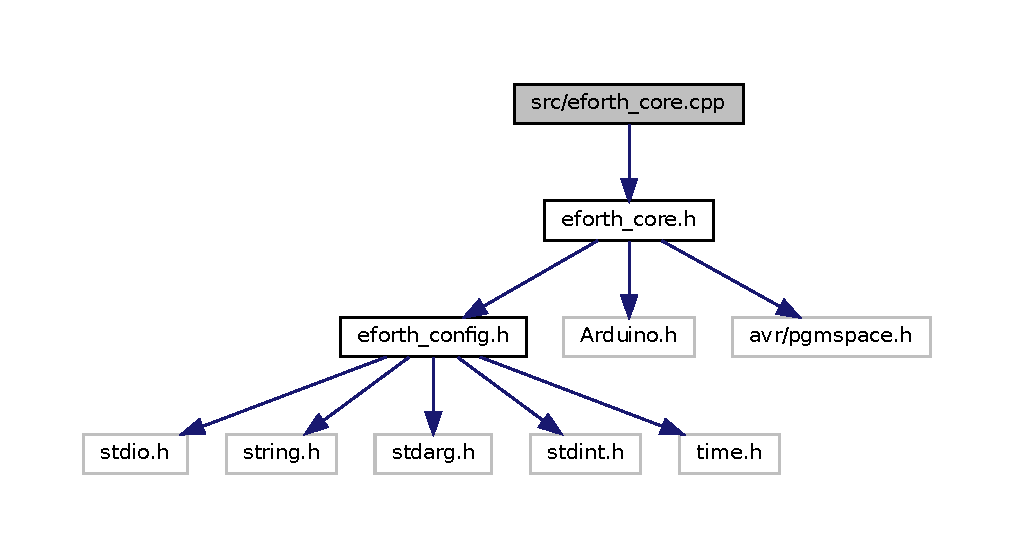
\includegraphics[width=350pt]{eforth__core_8cpp__incl}
\end{center}
\end{figure}
\doxysubsection*{Macros}
\begin{DoxyCompactItemize}
\item 
\#define \mbox{\hyperlink{eforth__core_8cpp_afc09b15fce90b9e00aa7277e7edd5c4e}{Y\+I\+E\+L\+D\+\_\+\+P\+E\+R\+I\+OD}}~10
\end{DoxyCompactItemize}
\doxysubsection*{Functions}
\begin{DoxyCompactItemize}
\item 
void \mbox{\hyperlink{eforth__core_8cpp_acb5ba193e134c2a17c7a1bda39613b83}{sys\+\_\+info}} (\mbox{\hyperlink{eforth__core_8h_aa63ef7b996d5487ce35a5a66601f3e73}{U8}} $\ast$cdata, int sz)
\item 
void \mbox{\hyperlink{eforth__core_8cpp_aa084a3e268cc140b2c8602dc52396ce4}{ef\+\_\+yield}} ()
\item 
\mbox{\hyperlink{eforth__core_8h_aa63ef7b996d5487ce35a5a66601f3e73}{U8}} \mbox{\hyperlink{eforth__core_8cpp_a41032b0ebdc389f0c30d15b6b7e8b025}{ef\+\_\+getchar}} ()
\item 
void \mbox{\hyperlink{eforth__core_8cpp_a40485405ab5338788520ef0380b01b70}{ef\+\_\+putchar}} (char \mbox{\hyperlink{ceForth__33_8cpp_a089aacf63ed94ae0e667bb8f6db3e853}{c}})
\item 
void \mbox{\hyperlink{eforth__core_8cpp_a3be4743e748619321c1a4f95928e8de1}{ef\+\_\+setup}} (Stream \&io\+\_\+stream=Serial)
\item 
void \mbox{\hyperlink{eforth__core_8cpp_a1fb0d84284dc4203d4a4e4dbe8e07b29}{ef\+\_\+run}} ()
\end{DoxyCompactItemize}
\doxysubsection*{Variables}
\begin{DoxyCompactItemize}
\item 
static \mbox{\hyperlink{eforth__core_8h_aa63ef7b996d5487ce35a5a66601f3e73}{U8}} $\ast$ \mbox{\hyperlink{eforth__core_8cpp_a05c7bc09ead4e68622fbbeb7b8d1ecdf}{\+\_\+ram}}
\begin{DoxyCompactList}\small\item\em forth memory block dynamic allocated \end{DoxyCompactList}\item 
static Stream $\ast$ \mbox{\hyperlink{eforth__core_8cpp_a701d8d7ac1f23c7b361d62e89c06399b}{io}}
\begin{DoxyCompactList}\small\item\em console interface \end{DoxyCompactList}\item 
\mbox{\hyperlink{ceForth__33_8cpp_ac3df7cf3c8cb172a588adec881447d68}{U32}} \mbox{\hyperlink{eforth__core_8cpp_ab122f4898c37a0db81ea641558424375}{forth\+\_\+rom}} \mbox{[}$\,$\mbox{]}
\item 
\mbox{\hyperlink{ceForth__33_8cpp_ac3df7cf3c8cb172a588adec881447d68}{U32}} \mbox{\hyperlink{eforth__core_8cpp_a6fe6f33736fc0d8ed68fd74b454e00e7}{forth\+\_\+rom\+\_\+sz}}
\end{DoxyCompactItemize}


\doxysubsection{Detailed Description}
e\+Forth core controller module 



\doxysubsection{Macro Definition Documentation}
\mbox{\Hypertarget{eforth__core_8cpp_afc09b15fce90b9e00aa7277e7edd5c4e}\label{eforth__core_8cpp_afc09b15fce90b9e00aa7277e7edd5c4e}} 
\index{eforth\_core.cpp@{eforth\_core.cpp}!YIELD\_PERIOD@{YIELD\_PERIOD}}
\index{YIELD\_PERIOD@{YIELD\_PERIOD}!eforth\_core.cpp@{eforth\_core.cpp}}
\doxysubsubsection{\texorpdfstring{YIELD\_PERIOD}{YIELD\_PERIOD}}
{\footnotesize\ttfamily \#define Y\+I\+E\+L\+D\+\_\+\+P\+E\+R\+I\+OD~10}

e\+Forth yield to user tasks 

\doxysubsection{Function Documentation}
\mbox{\Hypertarget{eforth__core_8cpp_acb5ba193e134c2a17c7a1bda39613b83}\label{eforth__core_8cpp_acb5ba193e134c2a17c7a1bda39613b83}} 
\index{eforth\_core.cpp@{eforth\_core.cpp}!sys\_info@{sys\_info}}
\index{sys\_info@{sys\_info}!eforth\_core.cpp@{eforth\_core.cpp}}
\doxysubsubsection{\texorpdfstring{sys\_info()}{sys\_info()}}
{\footnotesize\ttfamily void sys\+\_\+info (\begin{DoxyParamCaption}\item[{\mbox{\hyperlink{eforth__core_8h_aa63ef7b996d5487ce35a5a66601f3e73}{U8}} $\ast$}]{cdata,  }\item[{int}]{sz }\end{DoxyParamCaption})}

display e\+Forth system information \mbox{\Hypertarget{eforth__core_8cpp_aa084a3e268cc140b2c8602dc52396ce4}\label{eforth__core_8cpp_aa084a3e268cc140b2c8602dc52396ce4}} 
\index{eforth\_core.cpp@{eforth\_core.cpp}!ef\_yield@{ef\_yield}}
\index{ef\_yield@{ef\_yield}!eforth\_core.cpp@{eforth\_core.cpp}}
\doxysubsubsection{\texorpdfstring{ef\_yield()}{ef\_yield()}}
{\footnotesize\ttfamily void ef\+\_\+yield (\begin{DoxyParamCaption}{ }\end{DoxyParamCaption})}

\mbox{\Hypertarget{eforth__core_8cpp_a41032b0ebdc389f0c30d15b6b7e8b025}\label{eforth__core_8cpp_a41032b0ebdc389f0c30d15b6b7e8b025}} 
\index{eforth\_core.cpp@{eforth\_core.cpp}!ef\_getchar@{ef\_getchar}}
\index{ef\_getchar@{ef\_getchar}!eforth\_core.cpp@{eforth\_core.cpp}}
\doxysubsubsection{\texorpdfstring{ef\_getchar()}{ef\_getchar()}}
{\footnotesize\ttfamily \mbox{\hyperlink{eforth__core_8h_aa63ef7b996d5487ce35a5a66601f3e73}{U8}} ef\+\_\+getchar (\begin{DoxyParamCaption}{ }\end{DoxyParamCaption})}

console input with yield \mbox{\Hypertarget{eforth__core_8cpp_a40485405ab5338788520ef0380b01b70}\label{eforth__core_8cpp_a40485405ab5338788520ef0380b01b70}} 
\index{eforth\_core.cpp@{eforth\_core.cpp}!ef\_putchar@{ef\_putchar}}
\index{ef\_putchar@{ef\_putchar}!eforth\_core.cpp@{eforth\_core.cpp}}
\doxysubsubsection{\texorpdfstring{ef\_putchar()}{ef\_putchar()}}
{\footnotesize\ttfamily void ef\+\_\+putchar (\begin{DoxyParamCaption}\item[{char}]{c }\end{DoxyParamCaption})}

output one char to console \mbox{\Hypertarget{eforth__core_8cpp_a3be4743e748619321c1a4f95928e8de1}\label{eforth__core_8cpp_a3be4743e748619321c1a4f95928e8de1}} 
\index{eforth\_core.cpp@{eforth\_core.cpp}!ef\_setup@{ef\_setup}}
\index{ef\_setup@{ef\_setup}!eforth\_core.cpp@{eforth\_core.cpp}}
\doxysubsubsection{\texorpdfstring{ef\_setup()}{ef\_setup()}}
{\footnotesize\ttfamily void ef\+\_\+setup (\begin{DoxyParamCaption}\item[{Stream \&}]{io\+\_\+stream = {\ttfamily Serial} }\end{DoxyParamCaption})}

setup (called by Arduino setup) \mbox{\Hypertarget{eforth__core_8cpp_a1fb0d84284dc4203d4a4e4dbe8e07b29}\label{eforth__core_8cpp_a1fb0d84284dc4203d4a4e4dbe8e07b29}} 
\index{eforth\_core.cpp@{eforth\_core.cpp}!ef\_run@{ef\_run}}
\index{ef\_run@{ef\_run}!eforth\_core.cpp@{eforth\_core.cpp}}
\doxysubsubsection{\texorpdfstring{ef\_run()}{ef\_run()}}
{\footnotesize\ttfamily void ef\+\_\+run (\begin{DoxyParamCaption}{ }\end{DoxyParamCaption})}

single step e\+Forth virtual machine 

\doxysubsection{Variable Documentation}
\mbox{\Hypertarget{eforth__core_8cpp_a05c7bc09ead4e68622fbbeb7b8d1ecdf}\label{eforth__core_8cpp_a05c7bc09ead4e68622fbbeb7b8d1ecdf}} 
\index{eforth\_core.cpp@{eforth\_core.cpp}!\_ram@{\_ram}}
\index{\_ram@{\_ram}!eforth\_core.cpp@{eforth\_core.cpp}}
\doxysubsubsection{\texorpdfstring{\_ram}{\_ram}}
{\footnotesize\ttfamily \mbox{\hyperlink{eforth__core_8h_aa63ef7b996d5487ce35a5a66601f3e73}{U8}}$\ast$ \+\_\+ram\hspace{0.3cm}{\ttfamily [static]}}



forth memory block dynamic allocated 

\mbox{\Hypertarget{eforth__core_8cpp_a701d8d7ac1f23c7b361d62e89c06399b}\label{eforth__core_8cpp_a701d8d7ac1f23c7b361d62e89c06399b}} 
\index{eforth\_core.cpp@{eforth\_core.cpp}!io@{io}}
\index{io@{io}!eforth\_core.cpp@{eforth\_core.cpp}}
\doxysubsubsection{\texorpdfstring{io}{io}}
{\footnotesize\ttfamily Stream$\ast$ io\hspace{0.3cm}{\ttfamily [static]}}



console interface 

\mbox{\Hypertarget{eforth__core_8cpp_ab122f4898c37a0db81ea641558424375}\label{eforth__core_8cpp_ab122f4898c37a0db81ea641558424375}} 
\index{eforth\_core.cpp@{eforth\_core.cpp}!forth\_rom@{forth\_rom}}
\index{forth\_rom@{forth\_rom}!eforth\_core.cpp@{eforth\_core.cpp}}
\doxysubsubsection{\texorpdfstring{forth\_rom}{forth\_rom}}
{\footnotesize\ttfamily const \mbox{\hyperlink{ceForth__33_8cpp_ac3df7cf3c8cb172a588adec881447d68}{U32}} forth\+\_\+rom}

\mbox{\Hypertarget{eforth__core_8cpp_a6fe6f33736fc0d8ed68fd74b454e00e7}\label{eforth__core_8cpp_a6fe6f33736fc0d8ed68fd74b454e00e7}} 
\index{eforth\_core.cpp@{eforth\_core.cpp}!forth\_rom\_sz@{forth\_rom\_sz}}
\index{forth\_rom\_sz@{forth\_rom\_sz}!eforth\_core.cpp@{eforth\_core.cpp}}
\doxysubsubsection{\texorpdfstring{forth\_rom\_sz}{forth\_rom\_sz}}
{\footnotesize\ttfamily \mbox{\hyperlink{ceForth__33_8cpp_ac3df7cf3c8cb172a588adec881447d68}{U32}} forth\+\_\+rom\+\_\+sz}


\hypertarget{eforth__core_8h}{}\doxysection{src/eforth\+\_\+core.h File Reference}
\label{eforth__core_8h}\index{src/eforth\_core.h@{src/eforth\_core.h}}


e\+Forth prototype and interface  


{\ttfamily \#include $<$stdio.\+h$>$}\newline
{\ttfamily \#include $<$string.\+h$>$}\newline
{\ttfamily \#include $<$stdarg.\+h$>$}\newline
{\ttfamily \#include $<$stdint.\+h$>$}\newline
{\ttfamily \#include $<$Arduino.\+h$>$}\newline
{\ttfamily \#include $<$avr/pgmspace.\+h$>$}\newline
{\ttfamily \#include $<$time.\+h$>$}\newline
Include dependency graph for eforth\+\_\+core.\+h\+:\nopagebreak
\begin{figure}[H]
\begin{center}
\leavevmode
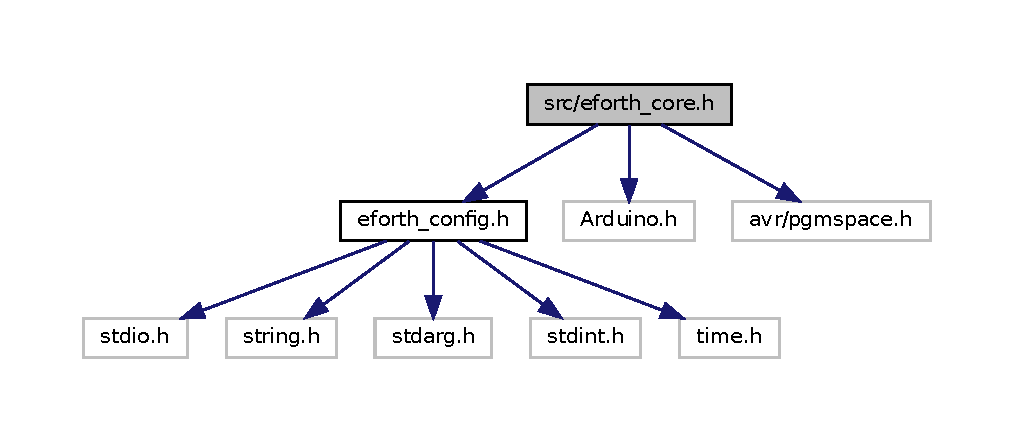
\includegraphics[width=350pt]{eforth__core_8h__incl}
\end{center}
\end{figure}
This graph shows which files directly or indirectly include this file\+:
\nopagebreak
\begin{figure}[H]
\begin{center}
\leavevmode
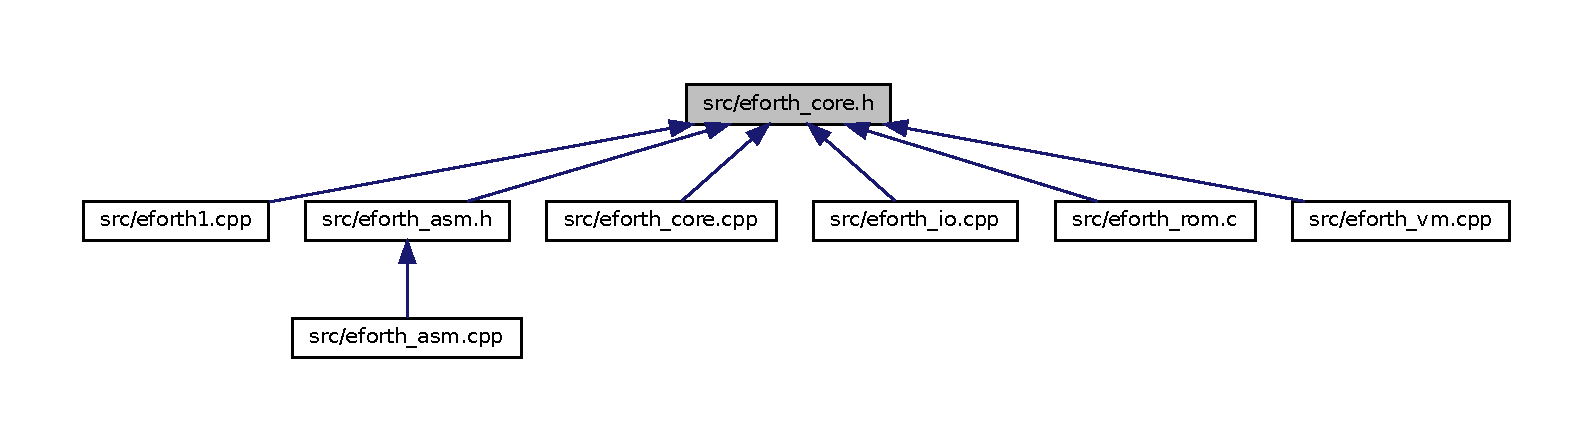
\includegraphics[width=350pt]{eforth__core_8h__dep__incl}
\end{center}
\end{figure}
\doxysubsection*{Macros}
\begin{DoxyCompactItemize}
\item 
\#define \mbox{\hyperlink{eforth__core_8h_af0b5cfa4242ae7f98ba80fd23ef8afa9}{A\+P\+P\+\_\+\+N\+A\+ME}}~\char`\"{}e\+Forth1\char`\"{}
\item 
\#define \mbox{\hyperlink{eforth__core_8h_aa9e8f3bb466bb421d13913df7aeaa20c}{M\+A\+J\+O\+R\+\_\+\+V\+E\+R\+S\+I\+ON}}~\char`\"{}v1\char`\"{}
\item 
\#define \mbox{\hyperlink{eforth__core_8h_a6094f5f4a8aa099faa6d80b4f020927b}{C\+A\+S\+E\+\_\+\+S\+E\+N\+S\+I\+T\+I\+VE}}~0
\item 
\#define \mbox{\hyperlink{eforth__core_8h_ae6bc65df3ece8101857357cbecc60d19}{A\+S\+M\+\_\+\+O\+N\+LY}}~0
\item 
\#define \mbox{\hyperlink{eforth__core_8h_a9d8d8ad7c0601f1313a9d026757f019a}{O\+P\+C\+O\+D\+ES}}
\end{DoxyCompactItemize}
\begin{Indent}\textbf{ Debug Tracing Flags}\par
\begin{DoxyCompactItemize}
\item 
\#define \mbox{\hyperlink{eforth__core_8h_afd97bab563464ed479ba96d704adf0bc}{A\+S\+M\+\_\+\+T\+R\+A\+CE}}~0
\item 
\#define \mbox{\hyperlink{eforth__core_8h_a4e7ebf605b9379a385139d145f5b1fc5}{E\+X\+E\+\_\+\+T\+R\+A\+CE}}~0
\end{DoxyCompactItemize}
\end{Indent}
\begin{Indent}\textbf{ Capacity and Sizing}\par
{\em \begin{DoxyAttention}{Attention}
reassemble R\+OM needed if F\+O\+R\+T\+H\+\_\+\+T\+I\+B\+\_\+\+SZ or F\+O\+R\+T\+H\+\_\+\+P\+A\+D\+\_\+\+SZ changed 
\end{DoxyAttention}
}\begin{DoxyCompactItemize}
\item 
\#define \mbox{\hyperlink{eforth__core_8h_a483d8c32764af688ede31fdc4d9707dc}{C\+E\+L\+L\+SZ}}~2
\item 
\#define \mbox{\hyperlink{eforth__core_8h_a68b9e34d65501f01d02ed377146ef0bb}{F\+O\+R\+T\+H\+\_\+\+R\+O\+M\+\_\+\+SZ}}~0x2000
\item 
\#define \mbox{\hyperlink{eforth__core_8h_aff92e9d3a1f1b8f50e5f99f48e415b9a}{F\+O\+R\+T\+H\+\_\+\+D\+I\+C\+\_\+\+SZ}}~0x400
\item 
\#define \mbox{\hyperlink{eforth__core_8h_ae8b4d200001ac27b69d50b2aa3d659e7}{F\+O\+R\+T\+H\+\_\+\+U\+V\+A\+R\+\_\+\+SZ}}~0x20
\item 
\#define \mbox{\hyperlink{eforth__core_8h_ae1c5fa2ddd43bad831ec09b454a87476}{F\+O\+R\+T\+H\+\_\+\+S\+T\+A\+C\+K\+\_\+\+SZ}}~0xe0
\item 
\#define \mbox{\hyperlink{eforth__core_8h_ae58acffa6250f628ad15cdc182d146bc}{F\+O\+R\+T\+H\+\_\+\+T\+I\+B\+\_\+\+SZ}}~0x80
\item 
\#define \mbox{\hyperlink{eforth__core_8h_a2d3ef7004f16db9f741d7aa5351ebc5d}{F\+O\+R\+T\+H\+\_\+\+P\+A\+D\+\_\+\+SZ}}~0x20
\item 
\#define \mbox{\hyperlink{eforth__core_8h_ac13ec61d2b1799e4ab11371a4254e7dd}{F\+O\+R\+T\+H\+\_\+\+R\+A\+M\+\_\+\+SZ}}
\end{DoxyCompactItemize}
\end{Indent}
\begin{Indent}\textbf{ Memory Map Addressing}\par
{\em \begin{quote}
note\+: Forth only needs a few bytes for Arduino auto (on heap), but Serial default T\+X/\+RX buffers uses 0x40 $\ast$ 2 = 128 bytes

logic and stack op macros (processor dependent)

\end{quote}
}\begin{DoxyCompactItemize}
\item 
\#define \mbox{\hyperlink{eforth__core_8h_a8854972678927e0868e458eab4d789a2}{F\+O\+R\+T\+H\+\_\+\+B\+O\+O\+T\+\_\+\+A\+D\+DR}}~0x0000
\item 
\#define \mbox{\hyperlink{eforth__core_8h_a5f9cc7e4245085a5ddabcbcd07635aad}{F\+O\+R\+T\+H\+\_\+\+R\+A\+M\+\_\+\+A\+D\+DR}}~\mbox{\hyperlink{eforth__core_8h_a68b9e34d65501f01d02ed377146ef0bb}{F\+O\+R\+T\+H\+\_\+\+R\+O\+M\+\_\+\+SZ}}
\item 
\#define \mbox{\hyperlink{eforth__core_8h_a9574a362044eba73eb09283aaa5d6ad3}{F\+O\+R\+T\+H\+\_\+\+D\+I\+C\+\_\+\+A\+D\+DR}}~(\mbox{\hyperlink{eforth__core_8h_a5f9cc7e4245085a5ddabcbcd07635aad}{F\+O\+R\+T\+H\+\_\+\+R\+A\+M\+\_\+\+A\+D\+DR}}   + 0)
\item 
\#define \mbox{\hyperlink{eforth__core_8h_af15f803ea14ff0e9a3fa11fe533d0393}{F\+O\+R\+T\+H\+\_\+\+U\+V\+A\+R\+\_\+\+A\+D\+DR}}~(\mbox{\hyperlink{eforth__core_8h_a9574a362044eba73eb09283aaa5d6ad3}{F\+O\+R\+T\+H\+\_\+\+D\+I\+C\+\_\+\+A\+D\+DR}}   + \mbox{\hyperlink{eforth__core_8h_aff92e9d3a1f1b8f50e5f99f48e415b9a}{F\+O\+R\+T\+H\+\_\+\+D\+I\+C\+\_\+\+SZ}})
\item 
\#define \mbox{\hyperlink{eforth__core_8h_af278ea3f0013fa26db155c0945bcb9d2}{F\+O\+R\+T\+H\+\_\+\+S\+T\+A\+C\+K\+\_\+\+A\+D\+DR}}~(\mbox{\hyperlink{eforth__core_8h_af15f803ea14ff0e9a3fa11fe533d0393}{F\+O\+R\+T\+H\+\_\+\+U\+V\+A\+R\+\_\+\+A\+D\+DR}}  + \mbox{\hyperlink{eforth__core_8h_ae8b4d200001ac27b69d50b2aa3d659e7}{F\+O\+R\+T\+H\+\_\+\+U\+V\+A\+R\+\_\+\+SZ}})
\item 
\#define \mbox{\hyperlink{eforth__core_8h_a0ff79d0c91d8f4e7af41afdd399d28a4}{F\+O\+R\+T\+H\+\_\+\+S\+T\+A\+C\+K\+\_\+\+T\+OP}}~(\mbox{\hyperlink{eforth__core_8h_af278ea3f0013fa26db155c0945bcb9d2}{F\+O\+R\+T\+H\+\_\+\+S\+T\+A\+C\+K\+\_\+\+A\+D\+DR}} + \mbox{\hyperlink{eforth__core_8h_ae1c5fa2ddd43bad831ec09b454a87476}{F\+O\+R\+T\+H\+\_\+\+S\+T\+A\+C\+K\+\_\+\+SZ}})
\item 
\#define \mbox{\hyperlink{eforth__core_8h_a7b21761447b5ce2df53bcd72baa34c73}{F\+O\+R\+T\+H\+\_\+\+T\+I\+B\+\_\+\+A\+D\+DR}}~(\mbox{\hyperlink{eforth__core_8h_a0ff79d0c91d8f4e7af41afdd399d28a4}{F\+O\+R\+T\+H\+\_\+\+S\+T\+A\+C\+K\+\_\+\+T\+OP}})
\end{DoxyCompactItemize}
\end{Indent}
\begin{Indent}\textbf{ Logical}\par
{\em T\+R\+UE cannot use 1 because N\+O\+T(ffffffff)==0 while N\+O\+T(1)==ffffffff which does not need boolean op (i.\+e. in C) }\begin{DoxyCompactItemize}
\item 
\#define \mbox{\hyperlink{eforth__core_8h_aa8cecfc5c5c054d2875c03e77b7be15d}{T\+R\+UE}}~-\/1
\item 
\#define \mbox{\hyperlink{eforth__core_8h_aa93f0eb578d23995850d61f7d61c55c1}{F\+A\+L\+SE}}~0
\end{DoxyCompactItemize}
\end{Indent}
\begin{Indent}\textbf{ Arduino Support Macros}\par
\begin{DoxyCompactItemize}
\item 
\#define \mbox{\hyperlink{eforth__core_8h_a570713ca4a493fc4d2130a405f3b87ea}{L\+OG}}(s)~\mbox{\hyperlink{eforth1_8cpp_a701d8d7ac1f23c7b361d62e89c06399b}{io}}-\/$>$print(F(s))
\item 
\#define \mbox{\hyperlink{eforth__core_8h_ad1115aa0a8df497fe7c107d2ac3ab66e}{L\+O\+G\+\_\+C}}(c)~\mbox{\hyperlink{eforth__core_8h_a40485405ab5338788520ef0380b01b70}{ef\+\_\+putchar}}(c)
\item 
\#define \mbox{\hyperlink{eforth__core_8h_a8089c2bc0d4770d10e62c7d74031d497}{L\+O\+G\+\_\+V}}(s,  n)~\{ \mbox{\hyperlink{eforth1_8cpp_a701d8d7ac1f23c7b361d62e89c06399b}{io}}-\/$>$print(F(s)); \mbox{\hyperlink{eforth1_8cpp_a701d8d7ac1f23c7b361d62e89c06399b}{io}}-\/$>$print((\mbox{\hyperlink{eforth__core_8h_a149fe3b107a553d7f4a2fcf3adc02b6a}{DU}})n); \}
\item 
\#define \mbox{\hyperlink{eforth__core_8h_a58eef1717c4dffedd3a63d061ed1b4a5}{L\+O\+G\+\_\+H}}(s,  n)~\{ \mbox{\hyperlink{eforth1_8cpp_a701d8d7ac1f23c7b361d62e89c06399b}{io}}-\/$>$print(F(s)); \mbox{\hyperlink{eforth1_8cpp_a701d8d7ac1f23c7b361d62e89c06399b}{io}}-\/$>$print(n, H\+EX); \}
\item 
\#define \mbox{\hyperlink{eforth__core_8h_a60bc02dc3bbd02fe2c8f7472d473a659}{C\+LI}}()~cli()
\item 
\#define \mbox{\hyperlink{eforth__core_8h_a52e81e3198871fa5ae5c84580a12c032}{S\+EI}}()~sei()
\end{DoxyCompactItemize}
\end{Indent}
\doxysubsection*{Typedefs}
\begin{Indent}\textbf{ Portable Types}\par
\begin{DoxyCompactItemize}
\item 
typedef uint32\+\_\+t \mbox{\hyperlink{eforth__core_8h_a696390429f2f3b644bde8d0322a24124}{U32}}
\begin{DoxyCompactList}\small\item\em 32-\/bit unsigned integer \end{DoxyCompactList}\item 
typedef uint16\+\_\+t \mbox{\hyperlink{eforth__core_8h_a0a0a322d5fa4a546d293a77ba8b4a71f}{U16}}
\begin{DoxyCompactList}\small\item\em 16-\/bit unsigned integer \end{DoxyCompactList}\item 
typedef uint8\+\_\+t \mbox{\hyperlink{eforth__core_8h_aa63ef7b996d5487ce35a5a66601f3e73}{U8}}
\begin{DoxyCompactList}\small\item\em 8-\/bit unsigned integer \end{DoxyCompactList}\item 
typedef int32\+\_\+t \mbox{\hyperlink{eforth__core_8h_a39c786017723555afb9e8b85accec0de}{S32}}
\begin{DoxyCompactList}\small\item\em 32-\/bit signed integer \end{DoxyCompactList}\item 
typedef int16\+\_\+t \mbox{\hyperlink{eforth__core_8h_a6d241ad21a823c90d4835380787db5d4}{S16}}
\begin{DoxyCompactList}\small\item\em 16-\/bit signed integer \end{DoxyCompactList}\item 
typedef int8\+\_\+t \mbox{\hyperlink{eforth__core_8h_af1475a0bb1962ef08dd1f78bd5dba87a}{S8}}
\begin{DoxyCompactList}\small\item\em 8-\/bit signed integer \end{DoxyCompactList}\item 
typedef \mbox{\hyperlink{eforth__core_8h_a0a0a322d5fa4a546d293a77ba8b4a71f}{U16}} \mbox{\hyperlink{eforth__core_8h_a5fd90490ca5b2ceb72bf8b2c89a9634b}{IU}}
\begin{DoxyCompactList}\small\item\em instruction/address unit (16-\/bit) \end{DoxyCompactList}\item 
typedef \mbox{\hyperlink{eforth__core_8h_a6d241ad21a823c90d4835380787db5d4}{S16}} \mbox{\hyperlink{eforth__core_8h_a149fe3b107a553d7f4a2fcf3adc02b6a}{DU}}
\begin{DoxyCompactList}\small\item\em data/cell unit \end{DoxyCompactList}\end{DoxyCompactItemize}
\end{Indent}
\doxysubsection*{Functions}
\begin{Indent}\textbf{ interrupt handle routines}\par
\begin{DoxyCompactItemize}
\item 
void \mbox{\hyperlink{eforth__core_8h_a0132f57c344961e9ff4037dd06b06948}{intr\+\_\+reset}} ()
\begin{DoxyCompactList}\small\item\em reset interrupts \end{DoxyCompactList}\item 
\mbox{\hyperlink{eforth__core_8h_a0a0a322d5fa4a546d293a77ba8b4a71f}{U16}} \mbox{\hyperlink{eforth__core_8h_a93c9ba339402353230060b417633ccd4}{intr\+\_\+hits}} ()
\begin{DoxyCompactList}\small\item\em return interrupt hit flags \end{DoxyCompactList}\item 
void \mbox{\hyperlink{eforth__core_8h_ae7417b9670e9fc6ddc511e247b90e058}{intr\+\_\+service}} (void($\ast$cb)(\mbox{\hyperlink{eforth__core_8h_a0a0a322d5fa4a546d293a77ba8b4a71f}{U16}}))
\item 
void \mbox{\hyperlink{eforth__core_8h_ae02901fc00b0a504db693e560852481b}{intr\+\_\+add\+\_\+timer}} (\mbox{\hyperlink{eforth__core_8h_a0a0a322d5fa4a546d293a77ba8b4a71f}{U16}} hz10, \mbox{\hyperlink{eforth__core_8h_a0a0a322d5fa4a546d293a77ba8b4a71f}{U16}} xt)
\item 
void \mbox{\hyperlink{eforth__core_8h_ab0b4b6096f24d31ce113f65adb72125c}{intr\+\_\+add\+\_\+pci}} (\mbox{\hyperlink{eforth__core_8h_a0a0a322d5fa4a546d293a77ba8b4a71f}{U16}} pin, \mbox{\hyperlink{eforth__core_8h_a0a0a322d5fa4a546d293a77ba8b4a71f}{U16}} xt)
\item 
void \mbox{\hyperlink{eforth__core_8h_a8d82211db5e512fd289ddd16c3d608ae}{intr\+\_\+enable\+\_\+timer}} (\mbox{\hyperlink{eforth__core_8h_a0a0a322d5fa4a546d293a77ba8b4a71f}{U16}} f)
\item 
void \mbox{\hyperlink{eforth__core_8h_a18a475c1f5e15f4867d6974f8f0c1d43}{intr\+\_\+enable\+\_\+pci}} (\mbox{\hyperlink{eforth__core_8h_a0a0a322d5fa4a546d293a77ba8b4a71f}{U16}} f)
\end{DoxyCompactItemize}
\end{Indent}
\begin{Indent}\textbf{ e\+Forth Virtual Machine Functions}\par
\begin{DoxyCompactItemize}
\item 
void \mbox{\hyperlink{eforth__core_8h_aa4cce331b74c197758d0b9ada8d58002}{vm\+\_\+init}} (P\+G\+M\+\_\+P rom, \mbox{\hyperlink{eforth__core_8h_aa63ef7b996d5487ce35a5a66601f3e73}{U8}} $\ast$cdata, void $\ast$io\+\_\+stream)
\item 
void \mbox{\hyperlink{eforth__core_8h_af37f991d68804c00ec61aec541d1908e}{vm\+\_\+isr}} (\mbox{\hyperlink{eforth__core_8h_a0a0a322d5fa4a546d293a77ba8b4a71f}{U16}} xt)
\begin{DoxyCompactList}\small\item\em VM interrupt service routine. \end{DoxyCompactList}\item 
int \mbox{\hyperlink{eforth__core_8h_a1235c887d8bdb522e79d94afa74162c5}{vm\+\_\+outer}} ()
\begin{DoxyCompactList}\small\item\em Forth outer interpreter. \end{DoxyCompactList}\end{DoxyCompactItemize}
\end{Indent}
\begin{Indent}\textbf{ e\+Forth IO Functions}\par
\begin{DoxyCompactItemize}
\item 
char \mbox{\hyperlink{eforth__core_8h_ae7350dd92eb09ea9c2102562af1713a1}{ef\+\_\+getchar}} ()
\item 
void \mbox{\hyperlink{eforth__core_8h_a40485405ab5338788520ef0380b01b70}{ef\+\_\+putchar}} (char c)
\end{DoxyCompactItemize}
\end{Indent}
\begin{Indent}\textbf{ e\+Forth Assembler Functions}\par
\begin{DoxyCompactItemize}
\item 
int \mbox{\hyperlink{eforth__core_8h_a94e10412bf5e1f89d12efb94e80979c8}{ef\+\_\+assemble}} (\mbox{\hyperlink{eforth__core_8h_aa63ef7b996d5487ce35a5a66601f3e73}{U8}} $\ast$cdata)
\end{DoxyCompactItemize}
\end{Indent}


\doxysubsection{Detailed Description}
e\+Forth prototype and interface 



\doxysubsection{Macro Definition Documentation}
\mbox{\Hypertarget{eforth__core_8h_af0b5cfa4242ae7f98ba80fd23ef8afa9}\label{eforth__core_8h_af0b5cfa4242ae7f98ba80fd23ef8afa9}} 
\index{eforth\_core.h@{eforth\_core.h}!APP\_NAME@{APP\_NAME}}
\index{APP\_NAME@{APP\_NAME}!eforth\_core.h@{eforth\_core.h}}
\doxysubsubsection{\texorpdfstring{APP\_NAME}{APP\_NAME}}
{\footnotesize\ttfamily \#define A\+P\+P\+\_\+\+N\+A\+ME~\char`\"{}e\+Forth1\char`\"{}}

\mbox{\Hypertarget{eforth__core_8h_aa9e8f3bb466bb421d13913df7aeaa20c}\label{eforth__core_8h_aa9e8f3bb466bb421d13913df7aeaa20c}} 
\index{eforth\_core.h@{eforth\_core.h}!MAJOR\_VERSION@{MAJOR\_VERSION}}
\index{MAJOR\_VERSION@{MAJOR\_VERSION}!eforth\_core.h@{eforth\_core.h}}
\doxysubsubsection{\texorpdfstring{MAJOR\_VERSION}{MAJOR\_VERSION}}
{\footnotesize\ttfamily \#define M\+A\+J\+O\+R\+\_\+\+V\+E\+R\+S\+I\+ON~\char`\"{}v1\char`\"{}}

\mbox{\Hypertarget{eforth__core_8h_a6094f5f4a8aa099faa6d80b4f020927b}\label{eforth__core_8h_a6094f5f4a8aa099faa6d80b4f020927b}} 
\index{eforth\_core.h@{eforth\_core.h}!CASE\_SENSITIVE@{CASE\_SENSITIVE}}
\index{CASE\_SENSITIVE@{CASE\_SENSITIVE}!eforth\_core.h@{eforth\_core.h}}
\doxysubsubsection{\texorpdfstring{CASE\_SENSITIVE}{CASE\_SENSITIVE}}
{\footnotesize\ttfamily \#define C\+A\+S\+E\+\_\+\+S\+E\+N\+S\+I\+T\+I\+VE~0}

define case sensitivity \mbox{\Hypertarget{eforth__core_8h_ae6bc65df3ece8101857357cbecc60d19}\label{eforth__core_8h_ae6bc65df3ece8101857357cbecc60d19}} 
\index{eforth\_core.h@{eforth\_core.h}!ASM\_ONLY@{ASM\_ONLY}}
\index{ASM\_ONLY@{ASM\_ONLY}!eforth\_core.h@{eforth\_core.h}}
\doxysubsubsection{\texorpdfstring{ASM\_ONLY}{ASM\_ONLY}}
{\footnotesize\ttfamily \#define A\+S\+M\+\_\+\+O\+N\+LY~0}

create R\+OM only (i.\+e. no debugging) \mbox{\Hypertarget{eforth__core_8h_afd97bab563464ed479ba96d704adf0bc}\label{eforth__core_8h_afd97bab563464ed479ba96d704adf0bc}} 
\index{eforth\_core.h@{eforth\_core.h}!ASM\_TRACE@{ASM\_TRACE}}
\index{ASM\_TRACE@{ASM\_TRACE}!eforth\_core.h@{eforth\_core.h}}
\doxysubsubsection{\texorpdfstring{ASM\_TRACE}{ASM\_TRACE}}
{\footnotesize\ttfamily \#define A\+S\+M\+\_\+\+T\+R\+A\+CE~0}

assembler tracing flag \mbox{\Hypertarget{eforth__core_8h_a4e7ebf605b9379a385139d145f5b1fc5}\label{eforth__core_8h_a4e7ebf605b9379a385139d145f5b1fc5}} 
\index{eforth\_core.h@{eforth\_core.h}!EXE\_TRACE@{EXE\_TRACE}}
\index{EXE\_TRACE@{EXE\_TRACE}!eforth\_core.h@{eforth\_core.h}}
\doxysubsubsection{\texorpdfstring{EXE\_TRACE}{EXE\_TRACE}}
{\footnotesize\ttfamily \#define E\+X\+E\+\_\+\+T\+R\+A\+CE~0}

virtual machine execution tracing flag \mbox{\Hypertarget{eforth__core_8h_a483d8c32764af688ede31fdc4d9707dc}\label{eforth__core_8h_a483d8c32764af688ede31fdc4d9707dc}} 
\index{eforth\_core.h@{eforth\_core.h}!CELLSZ@{CELLSZ}}
\index{CELLSZ@{CELLSZ}!eforth\_core.h@{eforth\_core.h}}
\doxysubsubsection{\texorpdfstring{CELLSZ}{CELLSZ}}
{\footnotesize\ttfamily \#define C\+E\+L\+L\+SZ~2}

16-\/bit cell size ~\newline
 \mbox{\Hypertarget{eforth__core_8h_a68b9e34d65501f01d02ed377146ef0bb}\label{eforth__core_8h_a68b9e34d65501f01d02ed377146ef0bb}} 
\index{eforth\_core.h@{eforth\_core.h}!FORTH\_ROM\_SZ@{FORTH\_ROM\_SZ}}
\index{FORTH\_ROM\_SZ@{FORTH\_ROM\_SZ}!eforth\_core.h@{eforth\_core.h}}
\doxysubsubsection{\texorpdfstring{FORTH\_ROM\_SZ}{FORTH\_ROM\_SZ}}
{\footnotesize\ttfamily \#define F\+O\+R\+T\+H\+\_\+\+R\+O\+M\+\_\+\+SZ~0x2000}

size of R\+OM (for pre-\/defined words) \mbox{\Hypertarget{eforth__core_8h_aff92e9d3a1f1b8f50e5f99f48e415b9a}\label{eforth__core_8h_aff92e9d3a1f1b8f50e5f99f48e415b9a}} 
\index{eforth\_core.h@{eforth\_core.h}!FORTH\_DIC\_SZ@{FORTH\_DIC\_SZ}}
\index{FORTH\_DIC\_SZ@{FORTH\_DIC\_SZ}!eforth\_core.h@{eforth\_core.h}}
\doxysubsubsection{\texorpdfstring{FORTH\_DIC\_SZ}{FORTH\_DIC\_SZ}}
{\footnotesize\ttfamily \#define F\+O\+R\+T\+H\+\_\+\+D\+I\+C\+\_\+\+SZ~0x400}

size of dictionary space ~\newline
 \mbox{\Hypertarget{eforth__core_8h_ae8b4d200001ac27b69d50b2aa3d659e7}\label{eforth__core_8h_ae8b4d200001ac27b69d50b2aa3d659e7}} 
\index{eforth\_core.h@{eforth\_core.h}!FORTH\_UVAR\_SZ@{FORTH\_UVAR\_SZ}}
\index{FORTH\_UVAR\_SZ@{FORTH\_UVAR\_SZ}!eforth\_core.h@{eforth\_core.h}}
\doxysubsubsection{\texorpdfstring{FORTH\_UVAR\_SZ}{FORTH\_UVAR\_SZ}}
{\footnotesize\ttfamily \#define F\+O\+R\+T\+H\+\_\+\+U\+V\+A\+R\+\_\+\+SZ~0x20}

size of Forth user variables ~\newline
 \mbox{\Hypertarget{eforth__core_8h_ae1c5fa2ddd43bad831ec09b454a87476}\label{eforth__core_8h_ae1c5fa2ddd43bad831ec09b454a87476}} 
\index{eforth\_core.h@{eforth\_core.h}!FORTH\_STACK\_SZ@{FORTH\_STACK\_SZ}}
\index{FORTH\_STACK\_SZ@{FORTH\_STACK\_SZ}!eforth\_core.h@{eforth\_core.h}}
\doxysubsubsection{\texorpdfstring{FORTH\_STACK\_SZ}{FORTH\_STACK\_SZ}}
{\footnotesize\ttfamily \#define F\+O\+R\+T\+H\+\_\+\+S\+T\+A\+C\+K\+\_\+\+SZ~0xe0}

size of data/return stack ~\newline
 \mbox{\Hypertarget{eforth__core_8h_ae58acffa6250f628ad15cdc182d146bc}\label{eforth__core_8h_ae58acffa6250f628ad15cdc182d146bc}} 
\index{eforth\_core.h@{eforth\_core.h}!FORTH\_TIB\_SZ@{FORTH\_TIB\_SZ}}
\index{FORTH\_TIB\_SZ@{FORTH\_TIB\_SZ}!eforth\_core.h@{eforth\_core.h}}
\doxysubsubsection{\texorpdfstring{FORTH\_TIB\_SZ}{FORTH\_TIB\_SZ}}
{\footnotesize\ttfamily \#define F\+O\+R\+T\+H\+\_\+\+T\+I\+B\+\_\+\+SZ~0x80}

size of terminal input buffer ~\newline
 \mbox{\Hypertarget{eforth__core_8h_a2d3ef7004f16db9f741d7aa5351ebc5d}\label{eforth__core_8h_a2d3ef7004f16db9f741d7aa5351ebc5d}} 
\index{eforth\_core.h@{eforth\_core.h}!FORTH\_PAD\_SZ@{FORTH\_PAD\_SZ}}
\index{FORTH\_PAD\_SZ@{FORTH\_PAD\_SZ}!eforth\_core.h@{eforth\_core.h}}
\doxysubsubsection{\texorpdfstring{FORTH\_PAD\_SZ}{FORTH\_PAD\_SZ}}
{\footnotesize\ttfamily \#define F\+O\+R\+T\+H\+\_\+\+P\+A\+D\+\_\+\+SZ~0x20}

size of output pad (in D\+IC space ) ~\newline
 \mbox{\Hypertarget{eforth__core_8h_ac13ec61d2b1799e4ab11371a4254e7dd}\label{eforth__core_8h_ac13ec61d2b1799e4ab11371a4254e7dd}} 
\index{eforth\_core.h@{eforth\_core.h}!FORTH\_RAM\_SZ@{FORTH\_RAM\_SZ}}
\index{FORTH\_RAM\_SZ@{FORTH\_RAM\_SZ}!eforth\_core.h@{eforth\_core.h}}
\doxysubsubsection{\texorpdfstring{FORTH\_RAM\_SZ}{FORTH\_RAM\_SZ}}
{\footnotesize\ttfamily \#define F\+O\+R\+T\+H\+\_\+\+R\+A\+M\+\_\+\+SZ}

{\bfseries Value\+:}
\begin{DoxyCode}{0}
\DoxyCodeLine{        ( \(\backslash\)}
\DoxyCodeLine{        FORTH\_DIC\_SZ + \mbox{\hyperlink{eforth__core_8h_ae8b4d200001ac27b69d50b2aa3d659e7}{FORTH\_UVAR\_SZ}} + \mbox{\hyperlink{eforth__core_8h_ae1c5fa2ddd43bad831ec09b454a87476}{FORTH\_STACK\_SZ}} + \mbox{\hyperlink{eforth__core_8h_ae58acffa6250f628ad15cdc182d146bc}{FORTH\_TIB\_SZ}})}

\end{DoxyCode}
total R\+AM \mbox{\Hypertarget{eforth__core_8h_a8854972678927e0868e458eab4d789a2}\label{eforth__core_8h_a8854972678927e0868e458eab4d789a2}} 
\index{eforth\_core.h@{eforth\_core.h}!FORTH\_BOOT\_ADDR@{FORTH\_BOOT\_ADDR}}
\index{FORTH\_BOOT\_ADDR@{FORTH\_BOOT\_ADDR}!eforth\_core.h@{eforth\_core.h}}
\doxysubsubsection{\texorpdfstring{FORTH\_BOOT\_ADDR}{FORTH\_BOOT\_ADDR}}
{\footnotesize\ttfamily \#define F\+O\+R\+T\+H\+\_\+\+B\+O\+O\+T\+\_\+\+A\+D\+DR~0x0000}

\mbox{\Hypertarget{eforth__core_8h_a5f9cc7e4245085a5ddabcbcd07635aad}\label{eforth__core_8h_a5f9cc7e4245085a5ddabcbcd07635aad}} 
\index{eforth\_core.h@{eforth\_core.h}!FORTH\_RAM\_ADDR@{FORTH\_RAM\_ADDR}}
\index{FORTH\_RAM\_ADDR@{FORTH\_RAM\_ADDR}!eforth\_core.h@{eforth\_core.h}}
\doxysubsubsection{\texorpdfstring{FORTH\_RAM\_ADDR}{FORTH\_RAM\_ADDR}}
{\footnotesize\ttfamily \#define F\+O\+R\+T\+H\+\_\+\+R\+A\+M\+\_\+\+A\+D\+DR~\mbox{\hyperlink{eforth__core_8h_a68b9e34d65501f01d02ed377146ef0bb}{F\+O\+R\+T\+H\+\_\+\+R\+O\+M\+\_\+\+SZ}}}

\mbox{\Hypertarget{eforth__core_8h_a9574a362044eba73eb09283aaa5d6ad3}\label{eforth__core_8h_a9574a362044eba73eb09283aaa5d6ad3}} 
\index{eforth\_core.h@{eforth\_core.h}!FORTH\_DIC\_ADDR@{FORTH\_DIC\_ADDR}}
\index{FORTH\_DIC\_ADDR@{FORTH\_DIC\_ADDR}!eforth\_core.h@{eforth\_core.h}}
\doxysubsubsection{\texorpdfstring{FORTH\_DIC\_ADDR}{FORTH\_DIC\_ADDR}}
{\footnotesize\ttfamily \#define F\+O\+R\+T\+H\+\_\+\+D\+I\+C\+\_\+\+A\+D\+DR~(\mbox{\hyperlink{eforth__core_8h_a5f9cc7e4245085a5ddabcbcd07635aad}{F\+O\+R\+T\+H\+\_\+\+R\+A\+M\+\_\+\+A\+D\+DR}}   + 0)}

\mbox{\Hypertarget{eforth__core_8h_af15f803ea14ff0e9a3fa11fe533d0393}\label{eforth__core_8h_af15f803ea14ff0e9a3fa11fe533d0393}} 
\index{eforth\_core.h@{eforth\_core.h}!FORTH\_UVAR\_ADDR@{FORTH\_UVAR\_ADDR}}
\index{FORTH\_UVAR\_ADDR@{FORTH\_UVAR\_ADDR}!eforth\_core.h@{eforth\_core.h}}
\doxysubsubsection{\texorpdfstring{FORTH\_UVAR\_ADDR}{FORTH\_UVAR\_ADDR}}
{\footnotesize\ttfamily \#define F\+O\+R\+T\+H\+\_\+\+U\+V\+A\+R\+\_\+\+A\+D\+DR~(\mbox{\hyperlink{eforth__core_8h_a9574a362044eba73eb09283aaa5d6ad3}{F\+O\+R\+T\+H\+\_\+\+D\+I\+C\+\_\+\+A\+D\+DR}}   + \mbox{\hyperlink{eforth__core_8h_aff92e9d3a1f1b8f50e5f99f48e415b9a}{F\+O\+R\+T\+H\+\_\+\+D\+I\+C\+\_\+\+SZ}})}

\mbox{\Hypertarget{eforth__core_8h_af278ea3f0013fa26db155c0945bcb9d2}\label{eforth__core_8h_af278ea3f0013fa26db155c0945bcb9d2}} 
\index{eforth\_core.h@{eforth\_core.h}!FORTH\_STACK\_ADDR@{FORTH\_STACK\_ADDR}}
\index{FORTH\_STACK\_ADDR@{FORTH\_STACK\_ADDR}!eforth\_core.h@{eforth\_core.h}}
\doxysubsubsection{\texorpdfstring{FORTH\_STACK\_ADDR}{FORTH\_STACK\_ADDR}}
{\footnotesize\ttfamily \#define F\+O\+R\+T\+H\+\_\+\+S\+T\+A\+C\+K\+\_\+\+A\+D\+DR~(\mbox{\hyperlink{eforth__core_8h_af15f803ea14ff0e9a3fa11fe533d0393}{F\+O\+R\+T\+H\+\_\+\+U\+V\+A\+R\+\_\+\+A\+D\+DR}}  + \mbox{\hyperlink{eforth__core_8h_ae8b4d200001ac27b69d50b2aa3d659e7}{F\+O\+R\+T\+H\+\_\+\+U\+V\+A\+R\+\_\+\+SZ}})}

\mbox{\Hypertarget{eforth__core_8h_a0ff79d0c91d8f4e7af41afdd399d28a4}\label{eforth__core_8h_a0ff79d0c91d8f4e7af41afdd399d28a4}} 
\index{eforth\_core.h@{eforth\_core.h}!FORTH\_STACK\_TOP@{FORTH\_STACK\_TOP}}
\index{FORTH\_STACK\_TOP@{FORTH\_STACK\_TOP}!eforth\_core.h@{eforth\_core.h}}
\doxysubsubsection{\texorpdfstring{FORTH\_STACK\_TOP}{FORTH\_STACK\_TOP}}
{\footnotesize\ttfamily \#define F\+O\+R\+T\+H\+\_\+\+S\+T\+A\+C\+K\+\_\+\+T\+OP~(\mbox{\hyperlink{eforth__core_8h_af278ea3f0013fa26db155c0945bcb9d2}{F\+O\+R\+T\+H\+\_\+\+S\+T\+A\+C\+K\+\_\+\+A\+D\+DR}} + \mbox{\hyperlink{eforth__core_8h_ae1c5fa2ddd43bad831ec09b454a87476}{F\+O\+R\+T\+H\+\_\+\+S\+T\+A\+C\+K\+\_\+\+SZ}})}

\mbox{\Hypertarget{eforth__core_8h_a7b21761447b5ce2df53bcd72baa34c73}\label{eforth__core_8h_a7b21761447b5ce2df53bcd72baa34c73}} 
\index{eforth\_core.h@{eforth\_core.h}!FORTH\_TIB\_ADDR@{FORTH\_TIB\_ADDR}}
\index{FORTH\_TIB\_ADDR@{FORTH\_TIB\_ADDR}!eforth\_core.h@{eforth\_core.h}}
\doxysubsubsection{\texorpdfstring{FORTH\_TIB\_ADDR}{FORTH\_TIB\_ADDR}}
{\footnotesize\ttfamily \#define F\+O\+R\+T\+H\+\_\+\+T\+I\+B\+\_\+\+A\+D\+DR~(\mbox{\hyperlink{eforth__core_8h_a0ff79d0c91d8f4e7af41afdd399d28a4}{F\+O\+R\+T\+H\+\_\+\+S\+T\+A\+C\+K\+\_\+\+T\+OP}})}

\mbox{\Hypertarget{eforth__core_8h_aa8cecfc5c5c054d2875c03e77b7be15d}\label{eforth__core_8h_aa8cecfc5c5c054d2875c03e77b7be15d}} 
\index{eforth\_core.h@{eforth\_core.h}!TRUE@{TRUE}}
\index{TRUE@{TRUE}!eforth\_core.h@{eforth\_core.h}}
\doxysubsubsection{\texorpdfstring{TRUE}{TRUE}}
{\footnotesize\ttfamily \#define T\+R\+UE~-\/1}

\mbox{\Hypertarget{eforth__core_8h_aa93f0eb578d23995850d61f7d61c55c1}\label{eforth__core_8h_aa93f0eb578d23995850d61f7d61c55c1}} 
\index{eforth\_core.h@{eforth\_core.h}!FALSE@{FALSE}}
\index{FALSE@{FALSE}!eforth\_core.h@{eforth\_core.h}}
\doxysubsubsection{\texorpdfstring{FALSE}{FALSE}}
{\footnotesize\ttfamily \#define F\+A\+L\+SE~0}

\mbox{\Hypertarget{eforth__core_8h_a9d8d8ad7c0601f1313a9d026757f019a}\label{eforth__core_8h_a9d8d8ad7c0601f1313a9d026757f019a}} 
\index{eforth\_core.h@{eforth\_core.h}!OPCODES@{OPCODES}}
\index{OPCODES@{OPCODES}!eforth\_core.h@{eforth\_core.h}}
\doxysubsubsection{\texorpdfstring{OPCODES}{OPCODES}}
{\footnotesize\ttfamily \#define O\+P\+C\+O\+D\+ES}

Forth VM Opcodes (for Bytecode Assembler) \mbox{\Hypertarget{eforth__core_8h_a570713ca4a493fc4d2130a405f3b87ea}\label{eforth__core_8h_a570713ca4a493fc4d2130a405f3b87ea}} 
\index{eforth\_core.h@{eforth\_core.h}!LOG@{LOG}}
\index{LOG@{LOG}!eforth\_core.h@{eforth\_core.h}}
\doxysubsubsection{\texorpdfstring{LOG}{LOG}}
{\footnotesize\ttfamily \#define L\+OG(\begin{DoxyParamCaption}\item[{}]{s }\end{DoxyParamCaption})~\mbox{\hyperlink{eforth1_8cpp_a701d8d7ac1f23c7b361d62e89c06399b}{io}}-\/$>$print(F(s))}

\mbox{\Hypertarget{eforth__core_8h_ad1115aa0a8df497fe7c107d2ac3ab66e}\label{eforth__core_8h_ad1115aa0a8df497fe7c107d2ac3ab66e}} 
\index{eforth\_core.h@{eforth\_core.h}!LOG\_C@{LOG\_C}}
\index{LOG\_C@{LOG\_C}!eforth\_core.h@{eforth\_core.h}}
\doxysubsubsection{\texorpdfstring{LOG\_C}{LOG\_C}}
{\footnotesize\ttfamily \#define L\+O\+G\+\_\+C(\begin{DoxyParamCaption}\item[{}]{c }\end{DoxyParamCaption})~\mbox{\hyperlink{eforth__core_8h_a40485405ab5338788520ef0380b01b70}{ef\+\_\+putchar}}(c)}

\mbox{\Hypertarget{eforth__core_8h_a8089c2bc0d4770d10e62c7d74031d497}\label{eforth__core_8h_a8089c2bc0d4770d10e62c7d74031d497}} 
\index{eforth\_core.h@{eforth\_core.h}!LOG\_V@{LOG\_V}}
\index{LOG\_V@{LOG\_V}!eforth\_core.h@{eforth\_core.h}}
\doxysubsubsection{\texorpdfstring{LOG\_V}{LOG\_V}}
{\footnotesize\ttfamily \#define L\+O\+G\+\_\+V(\begin{DoxyParamCaption}\item[{}]{s,  }\item[{}]{n }\end{DoxyParamCaption})~\{ \mbox{\hyperlink{eforth1_8cpp_a701d8d7ac1f23c7b361d62e89c06399b}{io}}-\/$>$print(F(s)); \mbox{\hyperlink{eforth1_8cpp_a701d8d7ac1f23c7b361d62e89c06399b}{io}}-\/$>$print((\mbox{\hyperlink{eforth__core_8h_a149fe3b107a553d7f4a2fcf3adc02b6a}{DU}})n); \}}

\mbox{\Hypertarget{eforth__core_8h_a58eef1717c4dffedd3a63d061ed1b4a5}\label{eforth__core_8h_a58eef1717c4dffedd3a63d061ed1b4a5}} 
\index{eforth\_core.h@{eforth\_core.h}!LOG\_H@{LOG\_H}}
\index{LOG\_H@{LOG\_H}!eforth\_core.h@{eforth\_core.h}}
\doxysubsubsection{\texorpdfstring{LOG\_H}{LOG\_H}}
{\footnotesize\ttfamily \#define L\+O\+G\+\_\+H(\begin{DoxyParamCaption}\item[{}]{s,  }\item[{}]{n }\end{DoxyParamCaption})~\{ \mbox{\hyperlink{eforth1_8cpp_a701d8d7ac1f23c7b361d62e89c06399b}{io}}-\/$>$print(F(s)); \mbox{\hyperlink{eforth1_8cpp_a701d8d7ac1f23c7b361d62e89c06399b}{io}}-\/$>$print(n, H\+EX); \}}

\mbox{\Hypertarget{eforth__core_8h_a60bc02dc3bbd02fe2c8f7472d473a659}\label{eforth__core_8h_a60bc02dc3bbd02fe2c8f7472d473a659}} 
\index{eforth\_core.h@{eforth\_core.h}!CLI@{CLI}}
\index{CLI@{CLI}!eforth\_core.h@{eforth\_core.h}}
\doxysubsubsection{\texorpdfstring{CLI}{CLI}}
{\footnotesize\ttfamily \#define C\+LI(\begin{DoxyParamCaption}{ }\end{DoxyParamCaption})~cli()}

\mbox{\Hypertarget{eforth__core_8h_a52e81e3198871fa5ae5c84580a12c032}\label{eforth__core_8h_a52e81e3198871fa5ae5c84580a12c032}} 
\index{eforth\_core.h@{eforth\_core.h}!SEI@{SEI}}
\index{SEI@{SEI}!eforth\_core.h@{eforth\_core.h}}
\doxysubsubsection{\texorpdfstring{SEI}{SEI}}
{\footnotesize\ttfamily \#define S\+EI(\begin{DoxyParamCaption}{ }\end{DoxyParamCaption})~sei()}



\doxysubsection{Typedef Documentation}
\mbox{\Hypertarget{eforth__core_8h_a696390429f2f3b644bde8d0322a24124}\label{eforth__core_8h_a696390429f2f3b644bde8d0322a24124}} 
\index{eforth\_core.h@{eforth\_core.h}!U32@{U32}}
\index{U32@{U32}!eforth\_core.h@{eforth\_core.h}}
\doxysubsubsection{\texorpdfstring{U32}{U32}}
{\footnotesize\ttfamily typedef uint32\+\_\+t \mbox{\hyperlink{eforth__core_8h_a696390429f2f3b644bde8d0322a24124}{U32}}}



32-\/bit unsigned integer 

\mbox{\Hypertarget{eforth__core_8h_a0a0a322d5fa4a546d293a77ba8b4a71f}\label{eforth__core_8h_a0a0a322d5fa4a546d293a77ba8b4a71f}} 
\index{eforth\_core.h@{eforth\_core.h}!U16@{U16}}
\index{U16@{U16}!eforth\_core.h@{eforth\_core.h}}
\doxysubsubsection{\texorpdfstring{U16}{U16}}
{\footnotesize\ttfamily typedef uint16\+\_\+t \mbox{\hyperlink{eforth__core_8h_a0a0a322d5fa4a546d293a77ba8b4a71f}{U16}}}



16-\/bit unsigned integer 

\mbox{\Hypertarget{eforth__core_8h_aa63ef7b996d5487ce35a5a66601f3e73}\label{eforth__core_8h_aa63ef7b996d5487ce35a5a66601f3e73}} 
\index{eforth\_core.h@{eforth\_core.h}!U8@{U8}}
\index{U8@{U8}!eforth\_core.h@{eforth\_core.h}}
\doxysubsubsection{\texorpdfstring{U8}{U8}}
{\footnotesize\ttfamily typedef uint8\+\_\+t \mbox{\hyperlink{eforth__core_8h_aa63ef7b996d5487ce35a5a66601f3e73}{U8}}}



8-\/bit unsigned integer 

\mbox{\Hypertarget{eforth__core_8h_a39c786017723555afb9e8b85accec0de}\label{eforth__core_8h_a39c786017723555afb9e8b85accec0de}} 
\index{eforth\_core.h@{eforth\_core.h}!S32@{S32}}
\index{S32@{S32}!eforth\_core.h@{eforth\_core.h}}
\doxysubsubsection{\texorpdfstring{S32}{S32}}
{\footnotesize\ttfamily typedef int32\+\_\+t \mbox{\hyperlink{eforth__core_8h_a39c786017723555afb9e8b85accec0de}{S32}}}



32-\/bit signed integer 

\mbox{\Hypertarget{eforth__core_8h_a6d241ad21a823c90d4835380787db5d4}\label{eforth__core_8h_a6d241ad21a823c90d4835380787db5d4}} 
\index{eforth\_core.h@{eforth\_core.h}!S16@{S16}}
\index{S16@{S16}!eforth\_core.h@{eforth\_core.h}}
\doxysubsubsection{\texorpdfstring{S16}{S16}}
{\footnotesize\ttfamily typedef int16\+\_\+t \mbox{\hyperlink{eforth__core_8h_a6d241ad21a823c90d4835380787db5d4}{S16}}}



16-\/bit signed integer 

\mbox{\Hypertarget{eforth__core_8h_af1475a0bb1962ef08dd1f78bd5dba87a}\label{eforth__core_8h_af1475a0bb1962ef08dd1f78bd5dba87a}} 
\index{eforth\_core.h@{eforth\_core.h}!S8@{S8}}
\index{S8@{S8}!eforth\_core.h@{eforth\_core.h}}
\doxysubsubsection{\texorpdfstring{S8}{S8}}
{\footnotesize\ttfamily typedef int8\+\_\+t \mbox{\hyperlink{eforth__core_8h_af1475a0bb1962ef08dd1f78bd5dba87a}{S8}}}



8-\/bit signed integer 

\mbox{\Hypertarget{eforth__core_8h_a5fd90490ca5b2ceb72bf8b2c89a9634b}\label{eforth__core_8h_a5fd90490ca5b2ceb72bf8b2c89a9634b}} 
\index{eforth\_core.h@{eforth\_core.h}!IU@{IU}}
\index{IU@{IU}!eforth\_core.h@{eforth\_core.h}}
\doxysubsubsection{\texorpdfstring{IU}{IU}}
{\footnotesize\ttfamily typedef \mbox{\hyperlink{eforth__core_8h_a0a0a322d5fa4a546d293a77ba8b4a71f}{U16}} \mbox{\hyperlink{eforth__core_8h_a5fd90490ca5b2ceb72bf8b2c89a9634b}{IU}}}



instruction/address unit (16-\/bit) 

\mbox{\Hypertarget{eforth__core_8h_a149fe3b107a553d7f4a2fcf3adc02b6a}\label{eforth__core_8h_a149fe3b107a553d7f4a2fcf3adc02b6a}} 
\index{eforth\_core.h@{eforth\_core.h}!DU@{DU}}
\index{DU@{DU}!eforth\_core.h@{eforth\_core.h}}
\doxysubsubsection{\texorpdfstring{DU}{DU}}
{\footnotesize\ttfamily typedef \mbox{\hyperlink{eforth__core_8h_a6d241ad21a823c90d4835380787db5d4}{S16}} \mbox{\hyperlink{eforth__core_8h_a149fe3b107a553d7f4a2fcf3adc02b6a}{DU}}}



data/cell unit 



\doxysubsection{Function Documentation}
\mbox{\Hypertarget{eforth__core_8h_a0132f57c344961e9ff4037dd06b06948}\label{eforth__core_8h_a0132f57c344961e9ff4037dd06b06948}} 
\index{eforth\_core.h@{eforth\_core.h}!intr\_reset@{intr\_reset}}
\index{intr\_reset@{intr\_reset}!eforth\_core.h@{eforth\_core.h}}
\doxysubsubsection{\texorpdfstring{intr\_reset()}{intr\_reset()}}
{\footnotesize\ttfamily void intr\+\_\+reset (\begin{DoxyParamCaption}{ }\end{DoxyParamCaption})}



reset interrupts 

\mbox{\Hypertarget{eforth__core_8h_a93c9ba339402353230060b417633ccd4}\label{eforth__core_8h_a93c9ba339402353230060b417633ccd4}} 
\index{eforth\_core.h@{eforth\_core.h}!intr\_hits@{intr\_hits}}
\index{intr\_hits@{intr\_hits}!eforth\_core.h@{eforth\_core.h}}
\doxysubsubsection{\texorpdfstring{intr\_hits()}{intr\_hits()}}
{\footnotesize\ttfamily \mbox{\hyperlink{eforth__core_8h_a0a0a322d5fa4a546d293a77ba8b4a71f}{U16}} intr\+\_\+hits (\begin{DoxyParamCaption}{ }\end{DoxyParamCaption})}



return interrupt hit flags 

\begin{quote}
fetch interrupt hit flags \end{quote}
\mbox{\Hypertarget{eforth__core_8h_ae7417b9670e9fc6ddc511e247b90e058}\label{eforth__core_8h_ae7417b9670e9fc6ddc511e247b90e058}} 
\index{eforth\_core.h@{eforth\_core.h}!intr\_service@{intr\_service}}
\index{intr\_service@{intr\_service}!eforth\_core.h@{eforth\_core.h}}
\doxysubsubsection{\texorpdfstring{intr\_service()}{intr\_service()}}
{\footnotesize\ttfamily void intr\+\_\+service (\begin{DoxyParamCaption}\item[{void($\ast$)(\mbox{\hyperlink{eforth__core_8h_a0a0a322d5fa4a546d293a77ba8b4a71f}{U16}})}]{cb }\end{DoxyParamCaption})}

\begin{quote}
service interrupt routines \end{quote}
\mbox{\Hypertarget{eforth__core_8h_ae02901fc00b0a504db693e560852481b}\label{eforth__core_8h_ae02901fc00b0a504db693e560852481b}} 
\index{eforth\_core.h@{eforth\_core.h}!intr\_add\_timer@{intr\_add\_timer}}
\index{intr\_add\_timer@{intr\_add\_timer}!eforth\_core.h@{eforth\_core.h}}
\doxysubsubsection{\texorpdfstring{intr\_add\_timer()}{intr\_add\_timer()}}
{\footnotesize\ttfamily void intr\+\_\+add\+\_\+timer (\begin{DoxyParamCaption}\item[{\mbox{\hyperlink{eforth__core_8h_a0a0a322d5fa4a546d293a77ba8b4a71f}{U16}}}]{hz10,  }\item[{\mbox{\hyperlink{eforth__core_8h_a0a0a322d5fa4a546d293a77ba8b4a71f}{U16}}}]{xt }\end{DoxyParamCaption})}

\begin{quote}
add timer interrupt service routine \end{quote}
\mbox{\Hypertarget{eforth__core_8h_ab0b4b6096f24d31ce113f65adb72125c}\label{eforth__core_8h_ab0b4b6096f24d31ce113f65adb72125c}} 
\index{eforth\_core.h@{eforth\_core.h}!intr\_add\_pci@{intr\_add\_pci}}
\index{intr\_add\_pci@{intr\_add\_pci}!eforth\_core.h@{eforth\_core.h}}
\doxysubsubsection{\texorpdfstring{intr\_add\_pci()}{intr\_add\_pci()}}
{\footnotesize\ttfamily void intr\+\_\+add\+\_\+pci (\begin{DoxyParamCaption}\item[{\mbox{\hyperlink{eforth__core_8h_a0a0a322d5fa4a546d293a77ba8b4a71f}{U16}}}]{p,  }\item[{\mbox{\hyperlink{eforth__core_8h_a0a0a322d5fa4a546d293a77ba8b4a71f}{U16}}}]{xt }\end{DoxyParamCaption})}

\begin{quote}
add pin change interrupt service routine \end{quote}
\mbox{\Hypertarget{eforth__core_8h_a8d82211db5e512fd289ddd16c3d608ae}\label{eforth__core_8h_a8d82211db5e512fd289ddd16c3d608ae}} 
\index{eforth\_core.h@{eforth\_core.h}!intr\_enable\_timer@{intr\_enable\_timer}}
\index{intr\_enable\_timer@{intr\_enable\_timer}!eforth\_core.h@{eforth\_core.h}}
\doxysubsubsection{\texorpdfstring{intr\_enable\_timer()}{intr\_enable\_timer()}}
{\footnotesize\ttfamily void intr\+\_\+enable\+\_\+timer (\begin{DoxyParamCaption}\item[{\mbox{\hyperlink{eforth__core_8h_a0a0a322d5fa4a546d293a77ba8b4a71f}{U16}}}]{f }\end{DoxyParamCaption})}

\begin{quote}
enable/disable timer2 interrupt \end{quote}
\mbox{\Hypertarget{eforth__core_8h_a18a475c1f5e15f4867d6974f8f0c1d43}\label{eforth__core_8h_a18a475c1f5e15f4867d6974f8f0c1d43}} 
\index{eforth\_core.h@{eforth\_core.h}!intr\_enable\_pci@{intr\_enable\_pci}}
\index{intr\_enable\_pci@{intr\_enable\_pci}!eforth\_core.h@{eforth\_core.h}}
\doxysubsubsection{\texorpdfstring{intr\_enable\_pci()}{intr\_enable\_pci()}}
{\footnotesize\ttfamily void intr\+\_\+enable\+\_\+pci (\begin{DoxyParamCaption}\item[{\mbox{\hyperlink{eforth__core_8h_a0a0a322d5fa4a546d293a77ba8b4a71f}{U16}}}]{f }\end{DoxyParamCaption})}

\begin{quote}
enable/disable pin change interrupt \end{quote}
\mbox{\Hypertarget{eforth__core_8h_aa4cce331b74c197758d0b9ada8d58002}\label{eforth__core_8h_aa4cce331b74c197758d0b9ada8d58002}} 
\index{eforth\_core.h@{eforth\_core.h}!vm\_init@{vm\_init}}
\index{vm\_init@{vm\_init}!eforth\_core.h@{eforth\_core.h}}
\doxysubsubsection{\texorpdfstring{vm\_init()}{vm\_init()}}
{\footnotesize\ttfamily void vm\+\_\+init (\begin{DoxyParamCaption}\item[{P\+G\+M\+\_\+P}]{rom,  }\item[{\mbox{\hyperlink{eforth__core_8h_aa63ef7b996d5487ce35a5a66601f3e73}{U8}} $\ast$}]{cdata,  }\item[{void $\ast$}]{io\+\_\+stream }\end{DoxyParamCaption})}


\begin{DoxyItemize}
\item resetting user variables
\end{DoxyItemize}
\begin{DoxyParams}{Parameters}
{\em rom} & pointer to Arduino flash memory block (R\+OM) \\
\hline
{\em cdata} & pointer to Arduino R\+AM block (R\+AM) \\
\hline
{\em io\+\_\+stream} & pointer to Stream object of Arduino \\
\hline
\end{DoxyParams}
\mbox{\Hypertarget{eforth__core_8h_af37f991d68804c00ec61aec541d1908e}\label{eforth__core_8h_af37f991d68804c00ec61aec541d1908e}} 
\index{eforth\_core.h@{eforth\_core.h}!vm\_isr@{vm\_isr}}
\index{vm\_isr@{vm\_isr}!eforth\_core.h@{eforth\_core.h}}
\doxysubsubsection{\texorpdfstring{vm\_isr()}{vm\_isr()}}
{\footnotesize\ttfamily void vm\+\_\+isr (\begin{DoxyParamCaption}\item[{\mbox{\hyperlink{eforth__core_8h_a0a0a322d5fa4a546d293a77ba8b4a71f}{U16}}}]{xt }\end{DoxyParamCaption})}



VM interrupt service routine. 

\begin{quote}
point to service function \end{quote}
\mbox{\Hypertarget{eforth__core_8h_a1235c887d8bdb522e79d94afa74162c5}\label{eforth__core_8h_a1235c887d8bdb522e79d94afa74162c5}} 
\index{eforth\_core.h@{eforth\_core.h}!vm\_outer@{vm\_outer}}
\index{vm\_outer@{vm\_outer}!eforth\_core.h@{eforth\_core.h}}
\doxysubsubsection{\texorpdfstring{vm\_outer()}{vm\_outer()}}
{\footnotesize\ttfamily int vm\+\_\+outer (\begin{DoxyParamCaption}{ }\end{DoxyParamCaption})}



Forth outer interpreter. 

\mbox{\Hypertarget{eforth__core_8h_ae7350dd92eb09ea9c2102562af1713a1}\label{eforth__core_8h_ae7350dd92eb09ea9c2102562af1713a1}} 
\index{eforth\_core.h@{eforth\_core.h}!ef\_getchar@{ef\_getchar}}
\index{ef\_getchar@{ef\_getchar}!eforth\_core.h@{eforth\_core.h}}
\doxysubsubsection{\texorpdfstring{ef\_getchar()}{ef\_getchar()}}
{\footnotesize\ttfamily char ef\+\_\+getchar (\begin{DoxyParamCaption}{ }\end{DoxyParamCaption})}

\begin{quote}
console input with yield \end{quote}
\mbox{\Hypertarget{eforth__core_8h_a40485405ab5338788520ef0380b01b70}\label{eforth__core_8h_a40485405ab5338788520ef0380b01b70}} 
\index{eforth\_core.h@{eforth\_core.h}!ef\_putchar@{ef\_putchar}}
\index{ef\_putchar@{ef\_putchar}!eforth\_core.h@{eforth\_core.h}}
\doxysubsubsection{\texorpdfstring{ef\_putchar()}{ef\_putchar()}}
{\footnotesize\ttfamily void ef\+\_\+putchar (\begin{DoxyParamCaption}\item[{char}]{c }\end{DoxyParamCaption})}

\begin{quote}
output one char to console \end{quote}
\mbox{\Hypertarget{eforth__core_8h_a94e10412bf5e1f89d12efb94e80979c8}\label{eforth__core_8h_a94e10412bf5e1f89d12efb94e80979c8}} 
\index{eforth\_core.h@{eforth\_core.h}!ef\_assemble@{ef\_assemble}}
\index{ef\_assemble@{ef\_assemble}!eforth\_core.h@{eforth\_core.h}}
\doxysubsubsection{\texorpdfstring{ef\_assemble()}{ef\_assemble()}}
{\footnotesize\ttfamily int ef\+\_\+assemble (\begin{DoxyParamCaption}\item[{\mbox{\hyperlink{eforth__core_8h_aa63ef7b996d5487ce35a5a66601f3e73}{U8}} $\ast$}]{cdata }\end{DoxyParamCaption})}


\begin{DoxyParams}{Parameters}
{\em cdata} & pointer to Arduino memory block where assembled data will be populated \\
\hline
\end{DoxyParams}

\hypertarget{eforth__rom_8c}{}\doxysection{src/eforth\+\_\+rom.c File Reference}
\label{eforth__rom_8c}\index{src/eforth\_rom.c@{src/eforth\_rom.c}}


e\+Forth R\+OM (loaded in Arduino Flash Memory)  


{\ttfamily \#include \char`\"{}eforth\+\_\+core.\+h\char`\"{}}\newline
Include dependency graph for eforth\+\_\+rom.\+c\+:\nopagebreak
\begin{figure}[H]
\begin{center}
\leavevmode
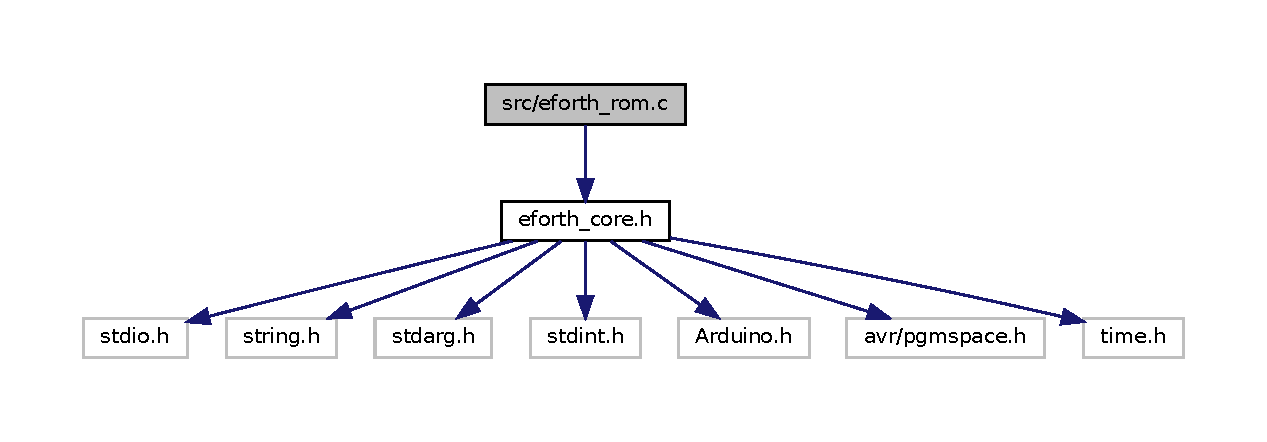
\includegraphics[width=350pt]{eforth__rom_8c__incl}
\end{center}
\end{figure}
\doxysubsection*{Variables}
\begin{DoxyCompactItemize}
\item 
const \mbox{\hyperlink{eforth__core_8h_a696390429f2f3b644bde8d0322a24124}{U32}} \mbox{\hyperlink{eforth1_8cpp_a6fe6f33736fc0d8ed68fd74b454e00e7}{forth\+\_\+rom\+\_\+sz}} \mbox{\hyperlink{eforth__rom_8c_a0babba59a58a58d5de2f517a9cd465b2}{P\+R\+O\+G\+M\+EM}} = 0xd7d
\end{DoxyCompactItemize}


\doxysubsection{Detailed Description}
e\+Forth R\+OM (loaded in Arduino Flash Memory) 

\begin{DoxyAttention}{Attention}
8K max R\+OM before changing F\+O\+R\+T\+H\+\_\+\+R\+O\+M\+\_\+\+SZ in \mbox{\hyperlink{eforth__core_8h}{eforth\+\_\+core.\+h}} 
\end{DoxyAttention}


\doxysubsection{Variable Documentation}
\mbox{\Hypertarget{eforth__rom_8c_a0babba59a58a58d5de2f517a9cd465b2}\label{eforth__rom_8c_a0babba59a58a58d5de2f517a9cd465b2}} 
\index{eforth\_rom.c@{eforth\_rom.c}!PROGMEM@{PROGMEM}}
\index{PROGMEM@{PROGMEM}!eforth\_rom.c@{eforth\_rom.c}}
\doxysubsubsection{\texorpdfstring{PROGMEM}{PROGMEM}}
{\footnotesize\ttfamily const \mbox{\hyperlink{eforth__core_8h_a696390429f2f3b644bde8d0322a24124}{U32}} \mbox{\hyperlink{eforth1_8cpp_ab122f4898c37a0db81ea641558424375}{forth\+\_\+rom}} \mbox{[}$\,$\mbox{]} P\+R\+O\+G\+M\+EM = 0xd7d}


\hypertarget{eforth__vm_8cpp}{}\doxysection{src/eforth\+\_\+vm.cpp File Reference}
\label{eforth__vm_8cpp}\index{src/eforth\_vm.cpp@{src/eforth\_vm.cpp}}


e\+Forth Virtual Machine module  


{\ttfamily \#include \char`\"{}eforth\+\_\+vm.\+h\char`\"{}}\newline
Include dependency graph for eforth\+\_\+vm.\+cpp\+:\nopagebreak
\begin{figure}[H]
\begin{center}
\leavevmode
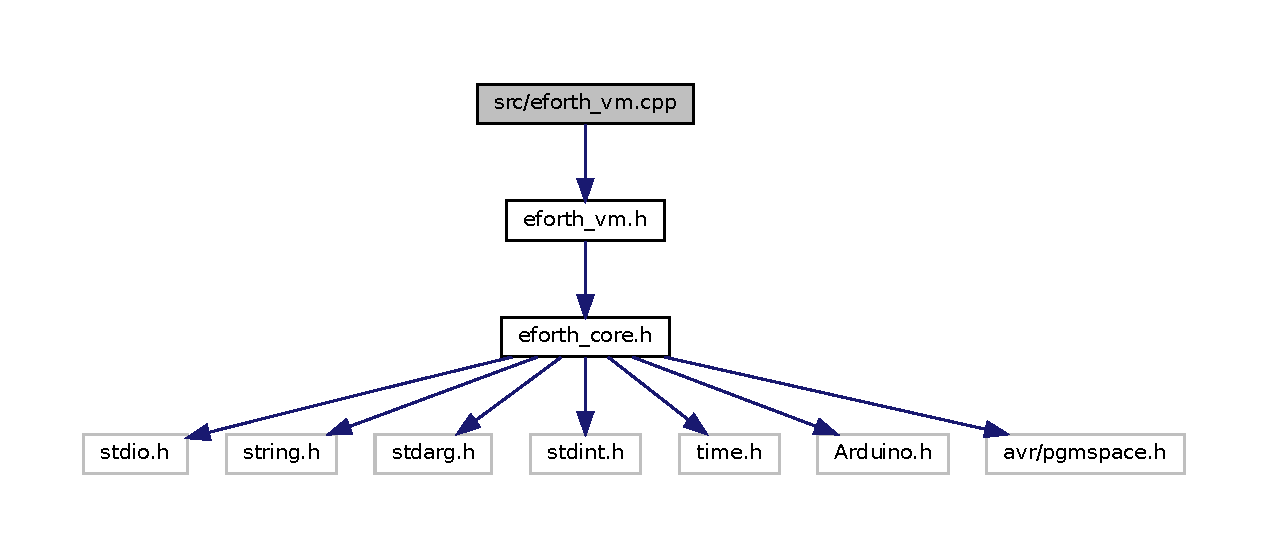
\includegraphics[width=350pt]{eforth__vm_8cpp__incl}
\end{center}
\end{figure}
\doxysubsection*{Namespaces}
\begin{DoxyCompactItemize}
\item 
 \mbox{\hyperlink{namespaceEfVM}{Ef\+VM}}
\end{DoxyCompactItemize}
\doxysubsection*{Macros}
\begin{DoxyCompactItemize}
\item 
\#define \mbox{\hyperlink{eforth__vm_8cpp_afc09b15fce90b9e00aa7277e7edd5c4e}{Y\+I\+E\+L\+D\+\_\+\+P\+E\+R\+I\+OD}}~100
\item 
\#define \mbox{\hyperlink{eforth__vm_8cpp_ab225fd437247be81c502ebd3b4857465}{Y\+I\+E\+LD}}()
\item 
\#define \mbox{\hyperlink{eforth__vm_8cpp_ac7635cecf944d5bfcc89665c08022828}{OP}}(name)~\&\&L\+\_\+\#\#name          /$\ast$$\ast$ redefined for label address     $\ast$/
\item 
\#define \mbox{\hyperlink{eforth__vm_8cpp_a694d28437d830c2e82367a5b56ae5163}{\+\_\+X}}(n,  code)~L\+\_\+\#\#n\+: \{ \mbox{\hyperlink{eforth__vm_8h_a3254550e1d6d185f6b3e69b2d6468343}{D\+E\+B\+UG}}(\char`\"{}\%s\char`\"{},\#n); code; continue; \}
\end{DoxyCompactItemize}
\doxysubsection*{Functions}
\begin{DoxyCompactItemize}
\item 
void \mbox{\hyperlink{namespaceEfVM_aaaa9f256ad4e73f2885577923fa23447}{Ef\+V\+M\+::\+\_\+init}} ()
\item 
void \mbox{\hyperlink{namespaceEfVM_a1149487a9866fbd91d4ccaf57eab9ea6}{Ef\+V\+M\+::\+\_\+yield}} ()
\begin{DoxyCompactList}\small\item\em \begin{quote}
yield to interrupt service \end{quote}
\end{DoxyCompactList}\item 
void \mbox{\hyperlink{namespaceEfVM_a2afadbdf0e72c8707edfebe583a5dfa6}{Ef\+V\+M\+::\+\_\+qrx}} ()
\begin{DoxyCompactList}\small\item\em \begin{quote}
( -- c ) fetch a char from console \end{quote}
\end{DoxyCompactList}\item 
void \mbox{\hyperlink{namespaceEfVM_ad93fbce2cb609c605aa8df2355c8e16b}{Ef\+V\+M\+::\+\_\+txsto}} ()
\begin{DoxyCompactList}\small\item\em \begin{quote}
(c -- ) send a char to console \end{quote}
\end{DoxyCompactList}\item 
void \mbox{\hyperlink{namespaceEfVM_a04b479eed7bc0fa0b9c8600f47c04cba}{Ef\+V\+M\+::\+\_\+ummod}} ()
\begin{DoxyCompactList}\small\item\em (udl udh u -- ur uq) unsigned double divided by a single \end{DoxyCompactList}\item 
void \mbox{\hyperlink{eforth__vm_8cpp_ab96d3e1cfedd27d24fea512540b32a98}{vm\+\_\+init}} (P\+G\+M\+\_\+P rom, \mbox{\hyperlink{eforth__core_8h_aa63ef7b996d5487ce35a5a66601f3e73}{U8}} $\ast$data, void $\ast$io\+\_\+stream)
\item 
void \mbox{\hyperlink{eforth__vm_8cpp_a8523598e2c601507492ae113056d7ef4}{\+\_\+ccall}} ()
\item 
void \mbox{\hyperlink{eforth__vm_8cpp_ac274d9a96db09bfc7ec4635be50d3aa5}{vm\+\_\+cfunc}} (int n, \mbox{\hyperlink{eforth__core_8h_a2d422d478f77fc6c4aa3c9538683829d}{C\+FP}} fp)
\begin{DoxyCompactList}\small\item\em \begin{quote}
function pointer \end{quote}
\end{DoxyCompactList}\item 
void \mbox{\hyperlink{eforth__vm_8cpp_a35fceadcc39370dc87d3be5608979925}{vm\+\_\+push}} (int v)
\begin{DoxyCompactList}\small\item\em push value onto VM data stack \end{DoxyCompactList}\item 
int \mbox{\hyperlink{eforth__vm_8cpp_a14b4544b998f4659f54969f571c58d8f}{vm\+\_\+pop}} ()
\begin{DoxyCompactList}\small\item\em pop T\+OS off VM data stack \end{DoxyCompactList}\end{DoxyCompactItemize}
\doxysubsection*{Variables}
\begin{DoxyCompactItemize}
\item 
static Stream $\ast$ \mbox{\hyperlink{namespaceEfVM_aa5ac1bb7ff2e93de1df7e220797fc690}{Ef\+V\+M\+::io}}
\item 
int \mbox{\hyperlink{namespaceEfVM_a09d628000e6b3bb7306a3bc9c3299efe}{Ef\+V\+M\+::\+\_\+yield\+\_\+cnt}} = 0
\begin{DoxyCompactList}\small\item\em interrupt service throttle counter \end{DoxyCompactList}\end{DoxyCompactItemize}
\begin{Indent}\textbf{ VM registers}\par
\begin{DoxyCompactItemize}
\item 
\mbox{\hyperlink{eforth__core_8h_a5fd90490ca5b2ceb72bf8b2c89a9634b}{IU}} \mbox{\hyperlink{namespaceEfVM_a34e9492841c1a98e29286c41dcdac10b}{Ef\+V\+M\+::\+IP}}
\begin{DoxyCompactList}\small\item\em instruction pointer, IU is 16-\/bit, opcode is 8-\/bit \end{DoxyCompactList}\item 
\mbox{\hyperlink{eforth__core_8h_a5fd90490ca5b2ceb72bf8b2c89a9634b}{IU}} \mbox{\hyperlink{namespaceEfVM_a4444ce01dd126290156b6339aedb281b}{Ef\+V\+M\+::\+PC}}
\begin{DoxyCompactList}\small\item\em program counter, IU is 16-\/bit \end{DoxyCompactList}\item 
\mbox{\hyperlink{eforth__core_8h_a149fe3b107a553d7f4a2fcf3adc02b6a}{DU}} $\ast$ \mbox{\hyperlink{namespaceEfVM_a9def3ba25dadbb291ebaee373982a18c}{Ef\+V\+M\+::\+DS}}
\begin{DoxyCompactList}\small\item\em data stack pointer, Dr. Ting\textquotesingle{}s stack \end{DoxyCompactList}\item 
\mbox{\hyperlink{eforth__core_8h_a149fe3b107a553d7f4a2fcf3adc02b6a}{DU}} $\ast$ \mbox{\hyperlink{namespaceEfVM_a44c4b6ad0dc45ad811db233793ab9ba8}{Ef\+V\+M\+::\+RS}}
\begin{DoxyCompactList}\small\item\em return stack pointer, Dr. Ting\textquotesingle{}s rack \end{DoxyCompactList}\item 
\mbox{\hyperlink{eforth__core_8h_a149fe3b107a553d7f4a2fcf3adc02b6a}{DU}} \mbox{\hyperlink{namespaceEfVM_a0d508bfbdbd7a09dcd56a24e3b6cb169}{Ef\+V\+M\+::top}}
\begin{DoxyCompactList}\small\item\em A\+LU (i.\+e. cached top of stack value) \end{DoxyCompactList}\item 
\mbox{\hyperlink{eforth__core_8h_a149fe3b107a553d7f4a2fcf3adc02b6a}{DU}} \mbox{\hyperlink{namespaceEfVM_a61aea862ab3bab556736663c844366c7}{Ef\+V\+M\+::rtop}}
\begin{DoxyCompactList}\small\item\em cached loop counter on return stack \end{DoxyCompactList}\item 
\mbox{\hyperlink{eforth__core_8h_a5fd90490ca5b2ceb72bf8b2c89a9634b}{IU}} \mbox{\hyperlink{namespaceEfVM_ad6bf1128d9ffa5007021ecabed123c74}{Ef\+V\+M\+::\+IR}}
\begin{DoxyCompactList}\small\item\em interrupt service routine \end{DoxyCompactList}\end{DoxyCompactItemize}
\end{Indent}
\begin{Indent}\textbf{ Memory Management Unit}\par
\begin{DoxyCompactItemize}
\item 
P\+G\+M\+\_\+P \mbox{\hyperlink{namespaceEfVM_a84f1ef51c831a00617756c690faa7194}{Ef\+V\+M\+::\+\_\+rom}}
\begin{DoxyCompactList}\small\item\em R\+OM, Forth word stored in Arduino Flash Memory. \end{DoxyCompactList}\item 
\mbox{\hyperlink{eforth__core_8h_aa63ef7b996d5487ce35a5a66601f3e73}{U8}} $\ast$ \mbox{\hyperlink{namespaceEfVM_a9f60f81681173bda3e807653f946a6f0}{Ef\+V\+M\+::\+\_\+data}}
\begin{DoxyCompactList}\small\item\em R\+AM, memory block for user define dictionary. \end{DoxyCompactList}\end{DoxyCompactItemize}
\end{Indent}
\begin{Indent}\textbf{ VM registers}\par
\begin{DoxyCompactItemize}
\item 
\mbox{\hyperlink{eforth__core_8h_a5fd90490ca5b2ceb72bf8b2c89a9634b}{IU}} \mbox{\hyperlink{namespaceEfVM_a34e9492841c1a98e29286c41dcdac10b}{Ef\+V\+M\+::\+IP}}
\begin{DoxyCompactList}\small\item\em instruction pointer, IU is 16-\/bit, opcode is 8-\/bit \end{DoxyCompactList}\item 
\mbox{\hyperlink{eforth__core_8h_a5fd90490ca5b2ceb72bf8b2c89a9634b}{IU}} \mbox{\hyperlink{namespaceEfVM_a4444ce01dd126290156b6339aedb281b}{Ef\+V\+M\+::\+PC}}
\begin{DoxyCompactList}\small\item\em program counter, IU is 16-\/bit \end{DoxyCompactList}\item 
\mbox{\hyperlink{eforth__core_8h_a149fe3b107a553d7f4a2fcf3adc02b6a}{DU}} $\ast$ \mbox{\hyperlink{namespaceEfVM_a9def3ba25dadbb291ebaee373982a18c}{Ef\+V\+M\+::\+DS}}
\begin{DoxyCompactList}\small\item\em data stack pointer, Dr. Ting\textquotesingle{}s stack \end{DoxyCompactList}\item 
\mbox{\hyperlink{eforth__core_8h_a149fe3b107a553d7f4a2fcf3adc02b6a}{DU}} $\ast$ \mbox{\hyperlink{namespaceEfVM_a44c4b6ad0dc45ad811db233793ab9ba8}{Ef\+V\+M\+::\+RS}}
\begin{DoxyCompactList}\small\item\em return stack pointer, Dr. Ting\textquotesingle{}s rack \end{DoxyCompactList}\item 
\mbox{\hyperlink{eforth__core_8h_a149fe3b107a553d7f4a2fcf3adc02b6a}{DU}} \mbox{\hyperlink{namespaceEfVM_a0d508bfbdbd7a09dcd56a24e3b6cb169}{Ef\+V\+M\+::top}}
\begin{DoxyCompactList}\small\item\em A\+LU (i.\+e. cached top of stack value) \end{DoxyCompactList}\item 
\mbox{\hyperlink{eforth__core_8h_a149fe3b107a553d7f4a2fcf3adc02b6a}{DU}} \mbox{\hyperlink{namespaceEfVM_a61aea862ab3bab556736663c844366c7}{Ef\+V\+M\+::rtop}}
\begin{DoxyCompactList}\small\item\em cached loop counter on return stack \end{DoxyCompactList}\item 
\mbox{\hyperlink{eforth__core_8h_a5fd90490ca5b2ceb72bf8b2c89a9634b}{IU}} \mbox{\hyperlink{namespaceEfVM_ad6bf1128d9ffa5007021ecabed123c74}{Ef\+V\+M\+::\+IR}}
\begin{DoxyCompactList}\small\item\em interrupt service routine \end{DoxyCompactList}\end{DoxyCompactItemize}
\end{Indent}
\begin{Indent}\textbf{ Memory Management Unit}\par
\begin{DoxyCompactItemize}
\item 
P\+G\+M\+\_\+P \mbox{\hyperlink{namespaceEfVM_a84f1ef51c831a00617756c690faa7194}{Ef\+V\+M\+::\+\_\+rom}}
\begin{DoxyCompactList}\small\item\em R\+OM, Forth word stored in Arduino Flash Memory. \end{DoxyCompactList}\item 
\mbox{\hyperlink{eforth__core_8h_aa63ef7b996d5487ce35a5a66601f3e73}{U8}} $\ast$ \mbox{\hyperlink{namespaceEfVM_a9f60f81681173bda3e807653f946a6f0}{Ef\+V\+M\+::\+\_\+data}}
\begin{DoxyCompactList}\small\item\em R\+AM, memory block for user define dictionary. \end{DoxyCompactList}\end{DoxyCompactItemize}
\end{Indent}


\doxysubsection{Detailed Description}
e\+Forth Virtual Machine module 

Revision Note\+: Threading model evolution 202212 Ef\+V\+M\+Sub module -\/ vtable subroutine calling 202301 indirect threading -\/ computed label jumping 202302 direct threading -\/ opcode =$>$ code(); continue = \$\+N\+E\+XT 

\doxysubsection{Macro Definition Documentation}
\mbox{\Hypertarget{eforth__vm_8cpp_afc09b15fce90b9e00aa7277e7edd5c4e}\label{eforth__vm_8cpp_afc09b15fce90b9e00aa7277e7edd5c4e}} 
\index{eforth\_vm.cpp@{eforth\_vm.cpp}!YIELD\_PERIOD@{YIELD\_PERIOD}}
\index{YIELD\_PERIOD@{YIELD\_PERIOD}!eforth\_vm.cpp@{eforth\_vm.cpp}}
\doxysubsubsection{\texorpdfstring{YIELD\_PERIOD}{YIELD\_PERIOD}}
{\footnotesize\ttfamily \#define Y\+I\+E\+L\+D\+\_\+\+P\+E\+R\+I\+OD~100}

\mbox{\Hypertarget{eforth__vm_8cpp_ab225fd437247be81c502ebd3b4857465}\label{eforth__vm_8cpp_ab225fd437247be81c502ebd3b4857465}} 
\index{eforth\_vm.cpp@{eforth\_vm.cpp}!YIELD@{YIELD}}
\index{YIELD@{YIELD}!eforth\_vm.cpp@{eforth\_vm.cpp}}
\doxysubsubsection{\texorpdfstring{YIELD}{YIELD}}
{\footnotesize\ttfamily \#define Y\+I\+E\+LD(\begin{DoxyParamCaption}{ }\end{DoxyParamCaption})}

{\bfseries Value\+:}
\begin{DoxyCode}{0}
\DoxyCodeLine{    \textcolor{keywordflow}{if} (!\mbox{\hyperlink{namespaceEfVM_ad6bf1128d9ffa5007021ecabed123c74}{IR}} \&\& ++\mbox{\hyperlink{namespaceEfVM_a09d628000e6b3bb7306a3bc9c3299efe}{\_yield\_cnt}} > \mbox{\hyperlink{eforth__vm_8cpp_afc09b15fce90b9e00aa7277e7edd5c4e}{YIELD\_PERIOD}}) \{ \(\backslash\)}
\DoxyCodeLine{        \_yield\_cnt = 0;                       \(\backslash\)}
\DoxyCodeLine{        \_yield();                             \(\backslash\)}
\DoxyCodeLine{    \}}

\end{DoxyCode}
\mbox{\Hypertarget{eforth__vm_8cpp_ac7635cecf944d5bfcc89665c08022828}\label{eforth__vm_8cpp_ac7635cecf944d5bfcc89665c08022828}} 
\index{eforth\_vm.cpp@{eforth\_vm.cpp}!OP@{OP}}
\index{OP@{OP}!eforth\_vm.cpp@{eforth\_vm.cpp}}
\doxysubsubsection{\texorpdfstring{OP}{OP}}
{\footnotesize\ttfamily \#define OP(\begin{DoxyParamCaption}\item[{}]{name }\end{DoxyParamCaption})~\&\&L\+\_\+\#\#name          /$\ast$$\ast$ redefined for label address     $\ast$/}

e\+Forth virtual machine outer interpreter (single-\/step) execution unit \begin{DoxyReturn}{Returns}
0 -\/ exit Note\+: vm\+\_\+outer -\/ computed label jumps (25\% faster than subroutine calls) continue in \mbox{\hyperlink{eforth__vm_8cpp_a694d28437d830c2e82367a5b56ae5163}{\+\_\+\+X()}} macro behaves as \$\+N\+E\+XT 
\end{DoxyReturn}
\mbox{\Hypertarget{eforth__vm_8cpp_a694d28437d830c2e82367a5b56ae5163}\label{eforth__vm_8cpp_a694d28437d830c2e82367a5b56ae5163}} 
\index{eforth\_vm.cpp@{eforth\_vm.cpp}!\_X@{\_X}}
\index{\_X@{\_X}!eforth\_vm.cpp@{eforth\_vm.cpp}}
\doxysubsubsection{\texorpdfstring{\_X}{\_X}}
{\footnotesize\ttfamily \#define \+\_\+X(\begin{DoxyParamCaption}\item[{}]{n,  }\item[{}]{code }\end{DoxyParamCaption})~L\+\_\+\#\#n\+: \{ \mbox{\hyperlink{eforth__vm_8h_a3254550e1d6d185f6b3e69b2d6468343}{D\+E\+B\+UG}}(\char`\"{}\%s\char`\"{},\#n); code; continue; \}}



\doxysubsection{Function Documentation}
\mbox{\Hypertarget{eforth__vm_8cpp_ab96d3e1cfedd27d24fea512540b32a98}\label{eforth__vm_8cpp_ab96d3e1cfedd27d24fea512540b32a98}} 
\index{eforth\_vm.cpp@{eforth\_vm.cpp}!vm\_init@{vm\_init}}
\index{vm\_init@{vm\_init}!eforth\_vm.cpp@{eforth\_vm.cpp}}
\doxysubsubsection{\texorpdfstring{vm\_init()}{vm\_init()}}
{\footnotesize\ttfamily void vm\+\_\+init (\begin{DoxyParamCaption}\item[{P\+G\+M\+\_\+P}]{rom,  }\item[{\mbox{\hyperlink{eforth__core_8h_aa63ef7b996d5487ce35a5a66601f3e73}{U8}} $\ast$}]{data,  }\item[{void $\ast$}]{io\+\_\+stream }\end{DoxyParamCaption})}


\begin{DoxyItemize}
\item resetting user variables
\end{DoxyItemize}\mbox{\Hypertarget{eforth__vm_8cpp_a8523598e2c601507492ae113056d7ef4}\label{eforth__vm_8cpp_a8523598e2c601507492ae113056d7ef4}} 
\index{eforth\_vm.cpp@{eforth\_vm.cpp}!\_ccall@{\_ccall}}
\index{\_ccall@{\_ccall}!eforth\_vm.cpp@{eforth\_vm.cpp}}
\doxysubsubsection{\texorpdfstring{\_ccall()}{\_ccall()}}
{\footnotesize\ttfamily void \+\_\+ccall (\begin{DoxyParamCaption}{ }\end{DoxyParamCaption})}

\begin{quote}
C interface implementation \end{quote}
T\+O\+DO\+: build formal C callstack construct \begin{quote}
fetch C function pointer \end{quote}


\begin{quote}
pop off T\+OS \end{quote}


\begin{quote}
call C function \end{quote}
\mbox{\Hypertarget{eforth__vm_8cpp_ac274d9a96db09bfc7ec4635be50d3aa5}\label{eforth__vm_8cpp_ac274d9a96db09bfc7ec4635be50d3aa5}} 
\index{eforth\_vm.cpp@{eforth\_vm.cpp}!vm\_cfunc@{vm\_cfunc}}
\index{vm\_cfunc@{vm\_cfunc}!eforth\_vm.cpp@{eforth\_vm.cpp}}
\doxysubsubsection{\texorpdfstring{vm\_cfunc()}{vm\_cfunc()}}
{\footnotesize\ttfamily void vm\+\_\+cfunc (\begin{DoxyParamCaption}\item[{int}]{n,  }\item[{\mbox{\hyperlink{eforth__core_8h_a2d422d478f77fc6c4aa3c9538683829d}{C\+FP}}}]{fp }\end{DoxyParamCaption})}



\begin{quote}
function pointer \end{quote}


assign C interface (in slot n) \begin{quote}
store C function pointer \end{quote}
\mbox{\Hypertarget{eforth__vm_8cpp_a35fceadcc39370dc87d3be5608979925}\label{eforth__vm_8cpp_a35fceadcc39370dc87d3be5608979925}} 
\index{eforth\_vm.cpp@{eforth\_vm.cpp}!vm\_push@{vm\_push}}
\index{vm\_push@{vm\_push}!eforth\_vm.cpp@{eforth\_vm.cpp}}
\doxysubsubsection{\texorpdfstring{vm\_push()}{vm\_push()}}
{\footnotesize\ttfamily void vm\+\_\+push (\begin{DoxyParamCaption}\item[{int}]{v }\end{DoxyParamCaption})}



push value onto VM data stack 

proxy to VM\mbox{\Hypertarget{eforth__vm_8cpp_a14b4544b998f4659f54969f571c58d8f}\label{eforth__vm_8cpp_a14b4544b998f4659f54969f571c58d8f}} 
\index{eforth\_vm.cpp@{eforth\_vm.cpp}!vm\_pop@{vm\_pop}}
\index{vm\_pop@{vm\_pop}!eforth\_vm.cpp@{eforth\_vm.cpp}}
\doxysubsubsection{\texorpdfstring{vm\_pop()}{vm\_pop()}}
{\footnotesize\ttfamily int vm\+\_\+pop (\begin{DoxyParamCaption}{ }\end{DoxyParamCaption})}



pop T\+OS off VM data stack 


%--- End generated contents ---

% Index
\backmatter
\newpage
\phantomsection
\clearemptydoublepage
\addcontentsline{toc}{chapter}{Index}
\printindex

\end{document}
